\documentclass[10pt]{article}
\usepackage[spanish]{babel}
\usepackage[utf8]{inputenc}
\usepackage[T1]{fontenc}
\usepackage{amsmath}
\usepackage{amsfonts}
\usepackage{amssymb}
\usepackage[version=4]{mhchem}
\usepackage{stmaryrd}
\usepackage{bbold}
\usepackage{graphicx}
\usepackage[export]{adjustbox}
\graphicspath{ {./images/} }
\usepackage{arydshln}

\begin{document}
\section*{Capítulo 1}
\section*{Programación lineal}
\section*{1. Introducción.}
En general, un problema de programación lineal consiste en maximizar o minimizar el valor de una función lineal $c . x=c_{1} x_{1}+\cdots+c_{n} x_{n}$ (a la que llamaremos el funcional) para ( $x_{1}, \ldots, x_{n}$ ) satisfaciendo un número finito de igualdades o desigualdades (a las que llamaremos restricciones) de alguno de los siguientes tipos:\\
$a_{1} x_{1}+\cdots+a_{n} x_{n}=b, \quad a_{1} x_{1}+\cdots+a_{n} x_{n} \leq b \quad$ о $\quad a_{1} x_{1}+\cdots+a_{n} x_{n} \geq b$\\
Cuando todas las ecuaciones sean del tipo $a_{i 1} x_{1}+\cdots+a_{i n} x_{n}=b_{i}(1 \leq i \leq m)$ usaremos la notación matricial $A x=b$, donde $A$ es la matriz de coeficientes $a_{i j}(1 \leq i \leq m, 1 \leq j \leq n), x=\left(x_{1}, \ldots, x_{n}\right)$, $b=\left(b_{1}, \ldots, b_{m}\right)$ y por abuso de notación estamos identificando $\mathbb{R}^{n}$ con $\mathbb{R}^{n \times 1}$. Análogamente, en lugar de $a_{i 1} x_{1}+\cdots+a_{i n} x_{n} \leq b_{i} \forall 1 \leq i \leq m$ escribiremos $A x \leq b$, etc. De esta manera, $x \geq 0$ significará $x_{j} \geq 0 \forall 1 \leq j \leq n$.\\
Veamos algunos ejemplos.\\
i) El problema del transporte.

Una empresa tiene dos plantas elaboradoras de tubos de acero, y tres centros de distribución. Una planta elabora 100 toneladas por día y la otra 200 . Cada centro demanda 75,125 y 100 toneladas por día respectivamente. Se estima que el costo $c_{i j}$ de llevar una tonelada de la planta $i$ al centro $j$ está dado por la matriz

$$
\left(\begin{array}{lll}
10 & 14 & 20 \\
12 & 20 & 17
\end{array}\right)
$$

Queremos determinar la cantidad $x_{i j}$ de toneladas a despachar por día de la planta $i$ al centro $j$ de manera tal que el costo total del transporte sea mínimo. Es decir, queremos minimizar la función lineal

$$
c . x=10 x_{11}+14 x_{12}+20 x_{13}+12 x_{21}+20 x_{22}+17 x_{23}
$$

con las restricciones

$$
\begin{aligned}
x_{11}+x_{12}+x_{13} & =100 \\
x_{21}+x_{22}+x_{23} & =200 \\
x_{11}+x_{21} & =75 \\
x_{12}+x_{22} & =125 \\
x_{13}+x_{23} & =100 \\
x_{i j} \geq 0 & \forall i, j
\end{aligned}
$$

Escrito matricialmente el problema es

$$
\begin{aligned}
& \min c x \\
& A x=b \\
& x \geq 0
\end{aligned}
$$

donde $A$ y $b$ son las matrices

$$
A=\left(\begin{array}{cccccc}
1 & 1 & 1 & 0 & 0 & 0 \\
0 & 0 & 0 & 1 & 1 & 1 \\
1 & 0 & 0 & 1 & 0 & 0 \\
0 & 1 & 0 & 0 & 1 & 0 \\
0 & 0 & 1 & 0 & 0 & 1
\end{array}\right) \quad \text { y } \quad b=\left(\begin{array}{c}
100 \\
200 \\
75 \\
125 \\
100
\end{array}\right)
$$

ii) El problema de la mezcla óptima de producción.

Una panadería elabora pan de 4 tipos, utilizando 6 ingredientes. Sea $a_{i j}$ la cantidad de kilos del ingrediente $i$ que se necesitan para elaborar un kilo de pan del tipo $j$ y sea $c_{j}$ la ganancia de vender un kilo de pan del tipo $j(1 \leq i \leq 6, \quad 1 \leq j \leq 4)$. Sabiendo que, en total, no pueden elaborarse más de 100 kilos de pan al día, y que diariamente se dispone de $b_{i}$ kilos del ingrediente $i$, se desea saber cuántos kilos de cada tipo de pan se deben elaborar por día para obtener la mayor ganancia.\\
Llamemos $x_{j}$ la cantidad de kg de pan del tipo $j$ que se elaborarán por día. Queremos maximizar la función lineal $c . x=c_{1} x_{1}+c_{2} x_{2}+c_{3} x_{3}+c_{4} x_{4}$, con las restricciones

$$
\begin{gathered}
a_{11} x_{1}+a_{12} x_{2}+a_{13} x_{3}+a_{14} x_{4} \leq b_{1} \\
a_{21} x_{1}+a_{22} x_{2}+a_{23} x_{3}+a_{24} x_{4} \leq b_{2} \\
a_{31} x_{1}+a_{32} x_{2}+a_{33} x_{3}+a_{34} x_{4} \leq b_{3} \\
a_{41} x_{1}+a_{42} x_{2}+a_{43} x_{3}+a_{44} x_{4} \leq b_{4} \\
a_{51} x_{1}+a_{52} x_{2}+a_{53} x_{3}+a_{54} x_{4} \leq b_{5} \\
a_{61} x_{1}+a_{62} x_{2}+a_{63} x_{3}+a_{64} x_{4} \leq b_{6} \\
x_{1}+x_{2}+x_{3}+x_{4} \leq 100 \\
x_{j} \geq 0 \quad \forall j
\end{gathered}
$$

es decir, queremos resolver el problema de programación lineal\\
donde $c=\left(c_{1}, c_{2}, c_{3}, c_{4}\right), A=\left(\begin{array}{cccc}a_{11} & a_{12} & a_{13} & a_{14} \\ a_{21} & a_{22} & a_{23} & a_{24} \\ a_{31} & a_{32} & a_{33} & a_{34} \\ a_{41} & a_{42} & a_{43} & a_{44} \\ a_{51} & a_{52} & a_{53} & a_{54} \\ a_{61} & a_{62} & a_{63} & a_{64} \\ 1 & 1 & 1 & 1\end{array}\right)$ y $b=\left(\begin{array}{c}b_{1} \\ b_{2} \\ b_{3} \\ b_{4} \\ b_{5} \\ b_{6} \\ 100\end{array}\right)$.\\
iii) El problema de la dieta.

Supongamos que queremos confeccionar una dieta con seis tipos de alimento, cada uno de ellos conteniendo cuatro clases de vitaminas. Sea $a_{i j}$ la cantidad de vitamina $i$ contenida en el alimento $j$ y sea $c_{j}$ el precio de un kilo de alimento $j$. Queremos saber cuántos kilos $x_{j}$ de cada alimento $j$ debemos incluír para garantizar que la dieta contenga por lo menos $b_{i}$ unidades de vitamina $i$ de manera tal que el costo total de los alimentos sea mínimo. Es decir, queremos minimizar la función lineal $c_{1} x_{1}+\cdots+c_{6} x_{6}$ sujeta a las restricciones $a_{i 1} x_{1}+\cdots+a_{i 6} x_{6} \geq b_{i}(1 \leq i \leq 4)$ y $x_{j} \geq 0(1 \leq j \leq 6)$. En otras palabras, queremos resolver el problema de programación lineal

$$
\begin{aligned}
& \min c x \\
& A x \geq b \\
& x \geq 0
\end{aligned}
$$

donde $c=\left(c_{1}, c_{2}, c_{3}, c_{4}, c_{5}, c_{6}\right), A=\left\|a_{i j}\right\| \mathrm{y} b=\left(\begin{array}{l}b_{1} \\ b_{2} \\ b_{3} \\ b_{4}\end{array}\right)$.

\section*{2. Forma standard.}
Observemos que una desigualdad del tipo

$$
a_{i 1} x_{1}+\cdots+a_{i n} x_{n} \leq b_{i}
$$

es equivalente a

$$
\left\{\begin{array}{l}
a_{i 1} x_{1}+\cdots+a_{i n} x_{n}+s_{i}=b_{i} \\
s_{i} \geq 0
\end{array}\right.
$$

La variable $s_{i}$ introducida se llama variable de holgura. De la misma manera, una desigualdad del tipo

$$
a_{i 1} x_{1}+\cdots+a_{i n} x_{n} \geq b_{i}
$$

puede ser reemplazada por

$$
\left\{\begin{array}{l}
a_{i 1} x_{1}+\cdots+a_{i n} x_{n}-s_{i}=b_{i} \\
s_{i} \geq 0
\end{array}\right.
$$

También observemos que si para algún $j$ no se pide la condición $x_{j} \geq 0$ entonces podemos reemplazar la variable $x_{j}$ por $y_{j}-z_{j}$ agregando las condiciones $y_{j} \geq 0$ y $z_{j} \geq 0$.\\
Por último, max $c x=-\min (-c) x$.\\
Todas estas observaciones muestran que cualquier problema de programación lineal puede ser planteado en la forma

$$
\begin{aligned}
& \min c x \\
& A x=b \\
& x \geq 0
\end{aligned}
$$

Esta forma de planteo del problema se denomina forma standard.

\section*{3. Teorema fundamental de la programación lineal.}
Definición 3.1. Un hiperplano en $\mathbb{R}^{n}$ es una variedad lineal de codimensión 1 , es decir, $\left\{x \in \mathbb{R}^{n} / a . x=k\right\}$, donde $a=\left(a_{1}, \ldots, a_{n}\right) \in \mathbb{R}^{n}, k \in \mathbb{R}$ y $a . x=a_{1} x_{1}+\cdots+a_{n} x_{n}$.\\
Cada hiperplano determina dos semiespacios: $\left\{x \in \mathbb{R}^{n} / a . x \leq k\right\}$ y $\left\{x \in \mathbb{R}^{n} / a . x \geq k\right\}$.\\
Un poliedro es la intersección de un número finito de semiespacios.\\
Observación 3.2. Notemos que el conjunto $\left\{x \in \mathbb{R}^{n} / a x=k\right\}$ es un poliedro ya que puede escribirse como intersección de los semiespacios $\left\{x \in \mathbb{R}^{n} / a x \leq k\right\}$ y $\left\{x \in \mathbb{R}^{n} / a x \geq k\right\}$. Además, es claro que la intersección de un número finito de poliedros es un poliedro. Esto muestra que el conjunto de todos los $x$ que satisfacen las restricciones de un problema de programación lineal es un poliedro. Luego, un problema de programación lineal consiste en maximizar o minimizar el valor de una función lineal sobre un poliedro.

Dado un problema de programación lineal, si el problema tiene una solución óptima entonces tiene una solución óptima en un punto extremo del poliedro. Antes de dar la definición rigurosa de punto extremo, veamos esto en un ejemplo.\\
Dado el problema de programación lineal

$$
\begin{aligned}
& \max 2 x_{1}-x_{2} \\
& x_{1}+2 x_{2} \leq 3 \\
& \left(x_{1}, x_{2}\right) \geq 0
\end{aligned}
$$

grafiquemos el poliedro $\left\{\left(x_{1}, x_{2}\right) \in \mathbb{R}^{2} / x_{1}+2 x_{2} \leq 3 \quad \wedge \quad x_{1} \geq 0 \quad \wedge \quad x_{2} \geq 0\right\}$ y las distintas rectas $2 x_{1}-x_{2}=k$\\
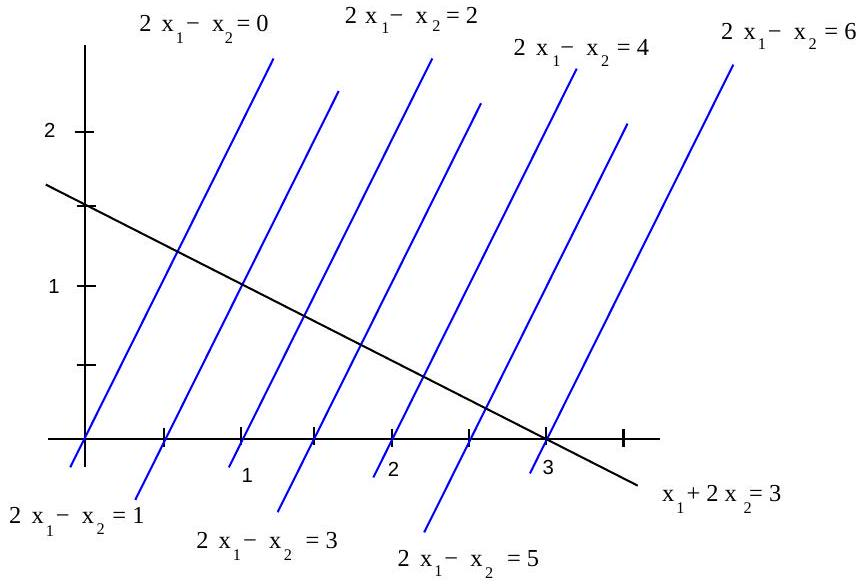
\includegraphics[max width=\textwidth, center]{2025_09_05_b12b6a6e1ba506f51b40g-04}

En este caso, los puntos extremos del poliedro son $(0,0)$, $(3,0)$ y $\left(0, \frac{3}{2}\right)$. Como se observa en la figura, la solución óptima $\left(x_{1}, x_{2}\right)=(3,0)$ es un punto extremo del poliedro.

Definición 3.3. Un subconjunto $\mathcal{K}$ de $\mathbb{R}^{n}$ se dice convexo sii $\alpha y+(1-\alpha) z \in \mathcal{K} \forall y, z \in \mathcal{K}, 0 \leq \alpha \leq 1$.\\
Dejamos a cargo del lector demostrar que un poliedro en $\mathbb{R}^{n}$ es un conjunto convexo.\\
Definición 3.4. Sea $\mathcal{K}$ un conjunto convexo en $\mathbb{R}^{n}$. Diremos que $x \in \mathcal{K}$ es un punto extremo si y sólo si no existen $y, z \in \mathcal{K}, \alpha \in \mathbb{R}$, con $y \neq z, 0<\alpha<1$ tales que $x=\alpha y+(1-\alpha) z$. En otras palabras, un punto de $K$ es un punto extremo si, cualesquiera sean $y, z \in K, y \neq z$, la única forma en que $x$ puede estar en el segmento que une $y$ con $z$ es que $x$ sea alguno de los extremos del segmento, es decir, $x=y$ o $x=z$.

Para lo que sigue necesitaremos definir los conceptos de solución básica y de solución factible de un problema de programación lineal que utilizaremos en las demostraciones.\\
Sea $A \in \mathbb{R}^{m \times n}$ una matriz de rango $m$ y sea $b \in \mathbb{R}^{m}$.\\
Definición 3.5. Diremos que $x \in \mathbb{R}^{n}$ es una solución básica de $A x=b$ sii $A x=b$ y existen $m$ índices $i_{1}, \ldots, i_{m}$ entre 1 y $n$ tales que $x_{j}=0 \forall j \neq i_{1}, \ldots, i_{m}$ y las columnas $i_{1}, \ldots, i_{m}$ de $A$ (que llamaremos la base) son linealmente independientes. Si $A x=b$ es el sistema lineal que aparece en las restricciones de un problema de programación lineal, diremos que $x$ es una solución básica del problema si $x$ es una solución básica de $A x=b$.\\
Observación 3.6. En la definición anterior hemos utilizado la misma letra $x$ para representar tanto a la variable como a la solución del sistema lineal $A x=b$. El lector atento sabrá distinguirlas en cada caso.\\
Observación 3.7. Si $A^{\prime} \in \mathbb{R}^{m \times n}$ es otra matriz de rango $m, b^{\prime} \in \mathbb{R}^{m}$ y los sistemas $A x=b$ y $A^{\prime} x=b^{\prime}$ son equivalentes entonces $x$ es una solución básica de $A x=b$ si y sólo si es una solución básica de $A^{\prime} x=b^{\prime}$.\\
Proposición 3.8. Dado $x$ tal que $A x=b$, si $\left\{j / x_{j} \neq 0\right\}=\left\{j_{1}, \ldots, j_{r}\right\}$ entonces se verifica: $x$ es una solución básica de $A x=b$ sii el conjunto formado por las columnas $j_{1}, \ldots, j_{r}$ de $A$ es linealmente independiente.\\
Demostración: $(\Longrightarrow)$ Sean $i_{1}, \ldots, i_{m}$ tales que $x_{j}=0$ para todo $j \neq i_{1}, \ldots, i_{m}$ y las columnas $i_{1}, \ldots, i_{m}$ de $A$ son linealmente independientes. Entonces $\left\{j_{1}, \ldots, j_{r}\right\} \subseteq\left\{i_{1}, \ldots, i_{m}\right\}$ de donde el conjunto formado por las columnas $j_{1}, \ldots, j_{r}$ de $A$ está contenido en el conjunto formado por las columnas $i_{1}, \ldots, i_{m}$ de $A$ y por lo tanto es linealmente independiente.\\
( $\Longleftarrow$ ) Si las columnas $j_{1}, \ldots, j_{r}$ de $A$ son linealmente independientes entonces $r \leq m$.\\
Si $r=m$ basta tomar $\left\{i_{1}, \ldots, i_{m}\right\}=\left\{j_{1}, \ldots, j_{m}\right\}$.\\
Si fuese $r<m$, como $A$ tiene rango $m$ entonces existen $j_{r+1}, \ldots, j_{m}$ tales que las columnas $j_{1}, \ldots, j_{m}$ de $A$ son linealmente independientes y vale que $x_{j}=0$ para todo $j \neq j_{1}, \ldots, j_{m}$. Luego también en este caso resulta que $x$ es una solución básica.

Definición 3.9. Una solución básica $x$ de $A x=b$ se dice degenerada sii $\#\left\{j \mid x_{j} \neq 0\right\}<m$ (es decir, si $x_{i_{k}}=0$ para algún $1 \leq k \leq m$ ).\\
Observación 3.10. Sea $x$ una solución básica de $A x=b$ y sean $i_{1}, \ldots, i_{m}$ tales que $x_{j}=0 \forall j \neq i_{1}, \ldots, i_{m}$ y las columnas $i_{1}, \ldots, i_{m}$ de $A$ son linealmente independientes Entonces, si $B$ es la submatriz de $A$ formada por las columnas $i_{1}, \ldots, i_{m}$, resulta que $B$ es inversible, $x_{j}=0 \forall j \neq i_{1}, \ldots, i_{m} \mathrm{y}$

$$
\left(\begin{array}{c}
x_{i_{1}} \\
x_{i_{2}} \\
\vdots \\
x_{i_{m}}
\end{array}\right)=B^{-1} \cdot\left(\begin{array}{c}
b_{1} \\
b_{2} \\
\vdots \\
b_{m}
\end{array}\right)
$$

Proposición 3.11. El sistema lineal $A x=b$ tiene a lo sumo $\binom{n}{m}$ soluciones básicas.\\
Demostración: Para cada solución básica $x$ de $A x=b$, fijemos $i_{1}, \ldots, i_{m}$ tales que $x_{j}=0 \forall j \neq i_{1}, \ldots, i_{m}$ y las columnas $i_{1}, \ldots, i_{m}$ de $A$ son linealmente independientes.\\
Sea $B$ la matriz formada por las columnas $i_{1}, \ldots, i_{m}$ de $A$ y sea $\bar{b}=B^{-1} b$. Entonces, por la observación 3.10,

$$
x_{j}=\left\{\begin{array}{ll}
0 & \text { si } j \neq i_{1}, \ldots, i_{m} \\
\bar{b}_{k} & \text { si } j=i_{k}
\end{array} \quad(1 \leq k \leq m)\right.
$$

Esto dice que la aplicación $\psi$ del conjunto de soluciones básicas de $A x=b$ en el conjunto de los subconjuntos de $m$ elementos del conjunto $\{1,2, \ldots, n\}$ dada por

$$
\psi(x)=\left\{i_{1}, \ldots, i_{m}\right\}
$$

es inyectiva. En efecto, si $\psi(x)=\psi\left(x^{\prime}\right)=\left\{i_{1}, \ldots, i_{m}\right\}$ entonces

$$
x_{j}=\left\{\begin{array}{ll}
0 & \text { si } j \neq i_{1}, \ldots, i_{m} \\
\bar{b}_{k} & \text { si } j=i_{k}
\end{array} \quad(1 \leq k \leq m)\right.
$$

y también

$$
x_{j}^{\prime}=\left\{\begin{array}{ll}
0 & \text { si } j \neq i_{1}, \ldots, i_{m} \\
\bar{b}_{k} & \text { si } j=i_{k}
\end{array} \quad(1 \leq k \leq m)\right.
$$

pues $\bar{b}$ no depende de $x$ sino sólo de $A, b$ y de $i_{1}, \ldots, i_{m}$. Luego $x=x^{\prime}$. .\\
Definición 3.12. Dado un problema de programación lineal diremos que $x$ es una solución factible sii $x$ satisface las restricciones del problema.

Notemos que no siempre existen soluciones factibles porque, por ejemplo, el sistema lineal podría no tener solución. Pero también porque aunque las tuviera, podría ocurrir que ninguna de estas soluciones verificara el resto de las restricciones, situación que por ejemplo se da en el problema

$$
\begin{gathered}
\max 3 x_{1}-x_{2}+2 x_{3} \\
x_{1}+x_{2}-x_{3}=2 \\
x_{1}+x_{2}=1 \\
x \geq 0
\end{gathered}
$$

Por las observaciones hechas en la sección 2. vamos a restringirnos al estudio de problemas planteados en forma standard.\\
Sean $A \in \mathbb{R}^{m \times n}, b \in \mathbb{R}^{m}$ y $c \in \mathbb{R}^{n}$ y consideremos el problema de programación lineal en forma standard


\begin{gather*}
\min c x \\
A x=b  \tag{1}\\
x \geq 0
\end{gather*}


Probaremos que si (1) tiene una solución óptima entonces tiene una solución óptima en un punto extremo del poliedro $\left\{x \in \mathbb{R}^{n} / A x=b \wedge x \geq 0\right\}$.\\
Veamos que podemos suponer que $\operatorname{rg} A=m$. En efecto, si (1) tiene una solución óptima entonces el sistema $A x=b$ debe ser compatible. Luego, el rango de $A$ debe ser igual al rango de la matriz ampliada $[A \mid b]$. Si $\operatorname{rg} A<m$ entonces rg $[A \mid b]<m$. Sean $F_{1}, \ldots, F_{m}$ las filas de $[A \mid b]$. Sea $\left\{F_{j_{1}}, \ldots, F_{j_{r}}\right\} \subseteq\left\{F_{1}, \ldots, F_{m}\right\}$ una base del subespacio generado por $F_{1}, \ldots, F_{m}$ y sea $\left[A^{\prime} \mid b^{\prime}\right]$ la matriz cuyas filas son $F_{j_{1}}, \ldots, F_{j_{r}}$. Entonces los sistemas $A x=b$ y $A^{\prime} x=b^{\prime}$ son equivalentes. Luego podemos reemplazar $A x=b$ por $A^{\prime} x=b^{\prime}$ en (1) donde ahora $A^{\prime} \in \mathbb{R}^{r \times n}$ tiene rango $r$. Por lo tanto, de ahora en adelante supondremos que $A$ tiene rango $m$.

Teorema 3.13. Sea $\mathcal{K}$ el poliedro $\mathcal{K}=\left\{x \in \mathbb{R}^{n} / A x=b \quad \wedge \quad x \geq 0\right\}$. Entonces $x \in \mathbb{R}^{n}$ es una solución básica y factible de (1) si y sólo si $x$ es un punto extremo de $\mathcal{K}$.

\section*{Demostración:}
$(\Longrightarrow)$ Sea $x$ una solución básica y factible de (1) que es combinación convexa de dos soluciones factibles (notemos que $\mathcal{K}$ es el conjunto de soluciones factibles de (1)), es decir, $x=\alpha y+(1-\alpha) z$, con $y, z \in \mathcal{K}$ y $0<\alpha<1$ y probemos que entonces $y=z$.\\
Sean $i_{1}, \ldots, i_{m}$ tales que $x_{j}=0$ para todo $j \neq i_{1}, \ldots, i_{m}$ y las columnas $i_{1}, \ldots, i_{m}$ de $A$ son linealmente independientes.\\
Entonces la submatriz $B$ formada por las columnas $i_{1}, \ldots, i_{m}$ de $A$ es una matriz inversible.\\
Veamos que $y=z$, es decir que $y_{j}=z_{j}$ para todo $j$.\\
Si $j \neq i_{1}, \ldots, i_{m}$ entonces $0=x_{j}=\alpha y_{j}+(1-\alpha) z_{j}$ y como $y \geq 0, z \geq 0, \alpha>0$ y $(1-\alpha)>0$ entonces debe ser $y_{j}=0=z_{j}$.\\
Ahora, como $A y=b=A z$ y como $y_{j}=0=z_{j}$ para todo $j \neq i_{1}, \ldots, i_{m}$ entonces

$$
B \cdot\left(\begin{array}{c}
y_{i_{1}} \\
y_{i_{2}} \\
\vdots \\
y_{i_{m}}
\end{array}\right)=b=B \cdot\left(\begin{array}{c}
z_{i_{1}} \\
z_{i_{2}} \\
\vdots \\
z_{i_{m}}
\end{array}\right)
$$

de donde resulta que

$$
\left(\begin{array}{c}
y_{i_{1}} \\
y_{i_{2}} \\
\vdots \\
y_{i_{m}}
\end{array}\right)=B^{-1} \cdot b=\left(\begin{array}{c}
z_{i_{1}} \\
z_{i_{2}} \\
\vdots \\
z_{i_{m}}
\end{array}\right)
$$

Luego $y_{i}=z_{i}$ para todo $i$, es decir, $y=z$. Esto muestra que $x$ es un punto extremo de $\mathcal{K}$.\\
$(\Longleftarrow)$ Sea $x \in \mathcal{K}$ un punto extremo. Probaremos que $x$ es una solución básica. Sean $i_{1}, \ldots, i_{r}$ tales que $x_{j}=0 \forall j \neq i_{1}, \ldots, i_{r}$ y $x_{i_{1}}, \ldots, x_{i_{r}} \neq 0$. Luego $x_{i_{k}}>0$ para todo $k$ tal que $1 \leq k \leq r$.\\
Si $B$ es la submatriz de $A$ formada por las columnas $i_{1}, \ldots, i_{r}$ entonces, por la proposición 3.8., basta ver que las columnas de $B$ son linealmente independientes.\\
Supongamos que las columnas de $B$ son linealmente dependientes. Entonces existe $w \in \mathbb{R}^{r}$ tal que $w \neq 0$ y $B . w=0$. Sea $v \in \mathbb{R}^{n}$ definido por

$$
v_{j}= \begin{cases}w_{s} & \text { si } j=i_{s}(1 \leq s \leq r) \\ 0 & \text { si } j \neq i_{1}, \ldots, i_{r}\end{cases}
$$

Entonces $A v=0$ y $v \neq 0$. Sea $k$ tal que $0<k \leq \min _{1 \leq s \leq r}\left\{\frac{x_{i_{s}}}{\left|w_{s}\right|} / w_{s} \neq 0\right\}$. Notemos que un tal $k$ existe pues $x_{i_{s}}>0(1 \leq s \leq r)$ y $w \neq 0$.\\
Sean $y=x+k . v$ y $z=x-k . v$. Entonces $x=\frac{1}{2} y+\frac{1}{2} z, y \neq z$ y además $y, z \in \mathcal{K}$. En efecto, es claro que $A y=b=A z$. Veamos que $y, z \geq 0$. Si $j \neq i_{1}, \ldots, i_{r}$ entonces $y_{j}=0=z_{j}$. Sea entonces $s$ tal que $1 \leq s \leq r$. Como $k \leq \min _{1 \leq s \leq r}\left\{\frac{x_{i_{s}}}{\left|w_{s}\right|} / w_{s} \neq 0\right\}$, dado $s=1, \ldots, r$ se tiene\\
i) si $w_{s}>0$ entonces $k \leq \frac{x_{i_{s}}}{w_{s}}$. Luego $k \cdot w_{s} \leq x_{i_{s}}$ de donde $x_{i_{s}}-k \cdot w_{s} \geq 0$ y además $x_{i_{s}}+k \cdot w_{s} \geq 0$ ya que $x_{i_{s}}>0, k>0$ y $w_{s}>0$\\
ii) si $w_{s}<0$ entonces $k \leq \frac{x_{i_{s}}}{-w_{s}}$. Luego $-k \cdot w_{s} \leq x_{i_{s}}$ de donde $x_{i_{s}}+k \cdot w_{s} \geq 0$ y además $x_{i_{s}}-k \cdot w_{s} \geq 0$ ya que $x_{i_{s}}>0, k>0$ y $w_{s}<0$\\
Luego $y_{i_{s}}=x_{i_{s}}+k \cdot w_{s} \geq 0$ y $z_{i_{s}}=x_{i_{s}}-k \cdot w_{s} \geq 0$ para todo $1 \leq s \leq r$.\\
Hemos probado entonces que existen $y, z \in \mathcal{K}, y \neq z$ tal que $x=\frac{1}{2} y+\frac{1}{2} z$. Absurdo, pues esto contradice que $x$ sea un punto extremo de $\mathcal{K}$. Por lo tanto, las columnas de $B$ son linealmente independientes.

Ahora estamos en condiciones de probar el teorema fundamental de la programación lineal.\\
Teorema 3.14. Consideremos el problema de programación lineal en forma standard

$$
\begin{aligned}
& \min c x \\
& A x=b \\
& x \geq 0
\end{aligned}
$$

donde $A \in \mathbb{R}^{m \times n}$ tiene rango $m, b \in \mathbb{R}^{m}$ y $c \in \mathbb{R}^{n}$.\\
Entonces se verifican las dos condiciones siguientes\\
i) si el problema tiene una solución factible entonces tiene una solución básica y factible.\\
ii) si el problema tiene una solución óptima entonces tiene una solución óptima que es básica.

\section*{Demostración:}
i) Para cada $x$ solución factible sea $r(x)=\#\left\{j / x_{j} \neq 0\right\}$. Sea $r=\min \{r(x) / x$ es factible $\}$ y sea $x$ una solución factible tal que $r(x)=r$. Probaremos que $x$ es una solución básica. Si $\left\{j / x_{j} \neq 0\right\}=\left\{i_{1}, \ldots, i_{r}\right\}$ se tiene que $x_{j}=0 \forall j \neq i_{1}, \ldots, i_{r}$ y $x_{j}>0$ si $j=i_{1}, \ldots, i_{r}$.\\
Por la proposición 3.8., basta probar que las correspondientes columnas $i_{1}, \ldots, i_{r}$ de $A$ son linealmente independientes. Supongamos que no. Sea $B$ la submatriz de $A$ formada por estas columnas y sea $w \in \mathbb{R}^{r}$, $w \neq 0$ tal que $B w=0$.\\
Como $x_{i_{s}}>0(1 \leq s \leq r)$ podemos elegir $\lambda \in \mathbb{R}$ tal que $x_{i_{s}}+\lambda . w_{s} \geq 0$ para todo $1 \leq s \leq r$ y $x_{i_{s}}+\lambda . w_{s}=0$ para al menos un valor de $s=1, \ldots, r$. En efecto, dado que cuando $w_{s}=0$ la desigualdad vale pues $x_{i_{s}} \geq 0$, basta tomar $\lambda$ verificando

$$
\lambda \geq \frac{-x_{i_{s}}}{w_{s}} \text { para todo } s / w_{s}>0
$$

y

$$
\lambda \leq \frac{-x_{i_{s}}}{w_{s}} \text { para todo } s / w_{s}<0
$$

de manera tal que para algún valor de $s$ valga la igualdad. Luego basta tomar

$$
\lambda= \begin{cases}\max \left\{\frac{-x_{i_{s}}}{w_{s}} / w_{s}>0\right\} & \text { si } \exists w_{s}>0 \\ \min \left\{\frac{-x_{i_{s}}}{w_{s}} / w_{s}<0\right\} & \text { si } w_{s} \leq 0 \text { para todo } s\end{cases}
$$

Sea $v \in \mathbb{R}^{n}$ definido por

$$
v_{j}= \begin{cases}0 & \text { si } j \neq i_{1}, \ldots, i_{r} \\ w_{s} & \text { si } j=i_{s}, 1 \leq s \leq r\end{cases}
$$

Entonces $A v=0$ de donde $y=x+\lambda . v$ verifica $A y=b$ y como

$$
y_{j}= \begin{cases}0 & \text { si } j \neq i_{1}, \ldots, i_{r} \\ x_{i_{s}}+\lambda \cdot w_{s} & \text { si } j=i_{s}, 1 \leq s \leq r\end{cases}
$$

entonces $y \geq 0$.\\
Pero $y_{j}=0$ para $j \neq i_{1}, \ldots, i_{r}$ y para algún $i_{s}$. Esto muestra que $y$ es una solución factible tal que $r(y)<r$. Absurdo pues esto contradice la elección de $r$.\\
ii) Sea ahora $r=\min \{r(x) / x$ es una solución óptima $\}$ y sea $x$ óptimo tal que $r(x)=r$. Probaremos que $x$ es una solución básica. Si $\left\{j / x_{j} \neq 0\right\}=\left\{i_{1}, \ldots, i_{r}\right\}$ se tiene que $x_{j}=0 \forall j \neq i_{1}, \ldots, i_{r}$ y $x_{j}>0$ si $j=i_{1}, \ldots, i_{r}$. Como antes, basta ver que las columnas $i_{1}, \ldots, i_{r}$ de $A$ son linealmente independientes. Supongamos que no. Sea $B$ la submatriz de $A$ formadas por esas columnas y sea $w \in \mathbb{R}^{r}, w \neq 0$ tal que $B w=0$. Sea $v \in \mathbb{R}^{n}$ como en i), es decir,

$$
v_{j}= \begin{cases}0 & \text { si } j \neq i_{1}, \ldots, i_{r} \\ w_{s} & \text { si } j=i_{s}, 1 \leq s \leq r\end{cases}
$$

Luego $A v=0$.\\
Veamos ahora que $c v=0$. En efecto, supongamos que $c v \neq 0$.\\
Primer caso: si $c v>0$\\
Sea

$$
\mu= \begin{cases}\max \left\{\frac{-x_{i_{s}}}{w_{s}} / w_{s}>0\right\} & \text { si } \exists w_{s}>0 \\ -1 & \text { si } w_{s} \leq 0 \text { para todo } s\end{cases}
$$

Sea $y=x+\mu . v$. Entonces $A y=b$ y $c y=c x+\mu . c v<c x$ pues $\mu<0$. Además $y \geq 0$ pues $y_{j}=0$ para $j \neq i_{1}, \ldots, i_{r}$ y para $1 \leq s \leq r y_{i_{s}}=x_{i_{s}}+\mu . w_{s} \geq 0$ (para $s$ tal que $w_{s}>0$ por la definición de $\mu$ y para $s$ tal que $w_{s}<0$ porque $\mu<0$ ). Absurdo pues esto contradice el hecho de que $x$ es una solución óptima.\\
Segundo caso: si $c v<0$\\
Sea ahora

$$
\tau= \begin{cases}\min \left\{\frac{-x_{i_{s}}}{w_{s}} / w_{s}<0\right\} & \text { si } \exists w_{s}<0 \\ 1 & \text { si } w_{s} \geq 0 \text { para todo } s\end{cases}
$$

Tomando $y=x+\tau . v$ resulta que $A y=b$ y $c y=c x+\tau . c v<c x$ pues $\tau>0$ y además $y \geq 0$. Nuevamente esto es un absurdo pues $x$ era óptimo.\\
Luego, $c v=0$. Sea ahora $\lambda$ como en i) y sea también $y=x+\lambda . v$. Entonces resulta que $A y=b, y \geq 0$, $r(y)<r$ y $c y=c x$. Luego, $y$ es una solución óptima tal que $r(y)<r$. Absurdo, esto contradice la elección de $r$. ㅁ

Corolario 3.15. Si (1) tiene una solución óptima entonces tiene una solución óptima en un punto extremo del poliedro $\left\{x \in \mathbb{R}^{n} / A x=b \wedge x \geq 0\right\}$.

\section*{4. Dualidad.}
Consideremos los problemas de programación lineal

\[
\begin{array}{ccc}
\min c x & \max y b \\
A x \geq b & (P) & y A=c  \tag{D}\\
& & y \geq 0 \\
\text { (primal) } & & (\text { dual })
\end{array}
\]

donde $A \in \mathbb{R}^{m \times n}, c \in \mathbb{R}^{n}$ y $b \in \mathbb{R}^{m}$. En esta sección probaremos que si (P) tiene una solución óptima $x_{0}$ entonces (D) tiene una solución $y_{0}$ óptima y además se verifica que $c x_{0}=y_{0} b$. En este sentido, diremos que (P) y (D) son problemas duales. Para poder probar esto necesitaremos antes algunos resultados.

Teorema 4.1. (Teorema del hiperplano separador) Sea $\mathcal{Z}$ un conjunto convexo y cerrado en $\mathbb{R}^{n}$ y sea $c \in \mathbb{R}^{n}$ tal que $c \notin \mathcal{Z}$. Entonces existe un hiperplano $H=\left\{x \in \mathbb{R}^{n} / a x=b\right\}$ (donde $a \in \mathbb{R}^{n}, b \in \mathbb{R}$ y $a x$ denota el producto escalar $\langle a, x\rangle=a_{1} x_{1}+\cdots+a_{n} x_{n}$ ) que satisface\\
i) $c \in H$\\
ii) $a z>b$ para todo $z \in \mathcal{Z}$

\section*{Demostración:}
Sea $z_{0} \in \mathcal{Z}$ tal que $d\left(z_{0}, c\right)=d(\mathcal{Z}, c)$. Sea $a=z_{0}-c$ y sea $b=a . c=a_{1} c_{1}+\cdots+a_{n} c_{n}$. Veremos que $a . z \neq b$ para todo $z \in \mathcal{Z}$. Supongamos que no. Sea entonces $z \in \mathcal{Z}$ tal que $a . z=b$.\\
Notando que para $x, y \in \mathbb{R}^{n}$ el producto que hemos definido como $x . y=x_{1} y_{1} \cdots x_{n} y_{n}$ no es otra cosa que el producto escalar usual $\langle x, y\rangle$, se tiene que

$$
<z_{0}-c, z>=<a, z>=a . z=b=a . c=<a, c>=<z_{0}-c, c>
$$

de donde $\left\langle z_{0}-c, z\right\rangle=\left\langle z_{0}-c, c\right\rangle$. Esto significa que $\left\langle z_{0}-c, z-c\right\rangle=0$, es decir $z_{0}-c$ y $z-c$ son ortogonales.\\
Veremos ahora que entonces hay un punto en el segmento que une $z$ y $z_{0}$ que está más cerca de $c$ que $z_{0}$, es decir, mostraremos que existe $\lambda, 0<\lambda<1$ tal que $\lambda z+(1-\lambda) z_{0}$ está más cerca de $c$ que $z_{0}$.\\
La siguiente figura ilustra esta situación.\\
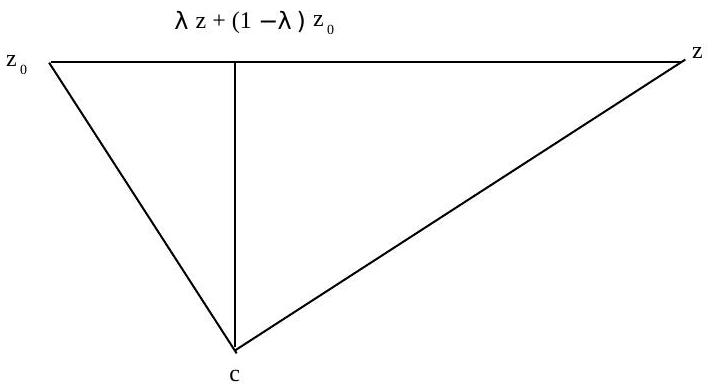
\includegraphics[max width=\textwidth, center]{2025_09_05_b12b6a6e1ba506f51b40g-09}

El segmento que une $z_{0}$ con $c$ es ortogonal al segmento que une $z$ con $c$.\\
Sea $\lambda=\frac{\left\|z_{0}-c\right\|^{2}}{\|z-c\|^{2}+\left\|z_{0}-c\right\|^{2}}$. Como $z_{0}-c$ y $z-c$ son no nulos pues $c \notin \mathcal{Z}$ entonces $0<\lambda<1$ y vale

$$
\lambda<\frac{2\left\|z_{0}-c\right\|^{2}}{\|z-c\|^{2}+\left\|z_{0}-c\right\|^{2}}
$$

Entonces

$$
\lambda\left(\|z-c\|^{2}+\left\|z_{0}-c\right\|^{2}\right)<2\left\|z_{0}-c\right\|^{2}
$$

de donde

$$
\lambda^{2}\left(\|z-c\|^{2}+\left\|z_{0}-c\right\|^{2}\right)<2 \lambda\left\|z_{0}-c\right\|^{2}
$$

lo que implica

$$
\lambda^{2}\left(\|z-c\|^{2}+\left\|z_{0}-c\right\|^{2}\right)-2 \lambda\left\|z_{0}-c\right\|^{2}<0
$$

con lo cual

$$
\lambda^{2}\|z-c\|^{2}-2 \lambda\left\|z_{0}-c\right\|^{2}+\lambda^{2}\left\|z_{0}-c\right\|^{2}<0
$$

y así

$$
\lambda^{2}\|z-c\|^{2}+(1-\lambda)^{2}\left\|z_{0}-c\right\|^{2}<\left\|z_{0}-c\right\|^{2}
$$

Como

$$
\left\|\lambda z+(1-\lambda) z_{0}-c\right\|^{2}=\left\|\lambda(z-c)+(1-\lambda)\left(z_{0}-c\right)\right\|^{2}=\lambda^{2}\|z-c\|^{2}+(1-\lambda)^{2}\left\|z_{0}-c\right\|^{2}
$$

pues $z_{0}-c$ y $z-c$ son ortogonales, entonces se tiene que $\left\|\lambda z+(1-\lambda) z_{0}-c\right\|^{2}<\left\|z_{0}-c\right\|^{2}$, de donde $d\left(\lambda z+(1-\lambda) z_{0}, c\right)<d(z, c)$.\\
Siendo $\mathcal{Z}$ convexo, $z, z_{0} \in \mathcal{Z}$ y $0<\lambda<1$ entonces $\bar{z}=\lambda z+(1-\lambda) z_{0} \in \mathcal{Z}$ y vale $d(\bar{z}, c)<d\left(z_{0}, c\right)=d(\mathcal{Z}, c)$ lo que es un absurdo. Luego debe ser $a . z \neq b$ para todo $z \in \mathcal{Z}$.

Veamos ahora que $a . z>b$ para todo $z \in \mathcal{Z}$ o $a z<b$ para todo $z \in \mathcal{Z}$. Supongamos que no. Sean $z_{1}, z_{2} \in \mathcal{Z}$ tales que $a . z_{1}>b$ y $a . z_{2}<b$. Probaremos que entonces existe $z \in \mathcal{Z}$ tal que $a . z=b$, cosa que vimos que no puede ocurrir.\\
Sea $\lambda=\frac{b-a . z_{2}}{a . z_{1}-a . z_{2}}$. (Notar que $a . z_{1} \neq a . z_{2}$ pues $a . z_{1}>b$ y $a . z_{2}<b$ ).\\
Dejamos a cargo del lector verificar que $0<\lambda<1$. Luego $z=\lambda z_{1}+(1-\lambda) z_{2} \in \mathcal{Z}$ y además vale $a . z=a .\left(\lambda z_{1}+(1-\lambda) z_{2}\right)=\lambda\left(a . z_{1}-a . z_{2}\right)+a . z_{2}=b$. Luego $a z>b$ para todo $z \in \mathcal{Z}$ o $a z<b$ para todo $z \in \mathcal{Z}$.\\
Si ocurre lo primero se obtiene el hiperplano buscado. Si ocurre lo segundo, entonces $-a z>-b$ para todo $z \in \mathcal{Z}$ y el hiperplano buscado es $H=\left\{x \in \mathbb{R}^{n} /(-a) x=(-b)\right\}$.\\
Ahora estamos en condiciones de probar el lema que necesitaremos para demostrar el teorema de dualidad.\\
Lema 4.2. (Lema de Farkas) Sean $U \in \mathbb{R}^{k \times n}, c \in \mathbb{R}^{n}$. Entonces son equivalentes:\\
i) $U . x \geq 0 \Longrightarrow c . x \geq 0$\\
ii) $\exists y \in \mathbb{R}^{k}, y \geq 0$ tal que $c=y . U$

\section*{Demostración:}
ii) $\Longrightarrow$ i) es trivial\\
i) $\Longrightarrow$ ii) Sea $\mathcal{Z}=\left\{z \in \mathbb{R}^{n} / z=y . U\right.$ para algún $\left.y \geq 0\right\}$.

Supongamos que ii) no vale. Entonces para todo $y \geq 0$ vale $y \cdot U \neq c$, es decir, $c \notin \mathcal{Z}$.\\
Como el conjunto $\mathcal{Z}$ es convexo y cerrado en $\mathbb{R}^{n}$ entonces por el teorema anterior existe un hiperplano $H=\left\{x \in \mathbb{R}^{n} / a x=b\right\}$ tal que $a c=b$ y $a z>b$ para todo $z \in \mathcal{Z}$. Por lo tanto $a c<a z$ para todo $z \in \mathcal{Z}$. En particular, como $0 \in \mathcal{Z}$ resulta que $c a=a c<0$.\\
Por otra parte, para todo $y \geq 0, y \cdot U \in \mathcal{Z}$. Luego, $b<a \cdot y \cdot U=y \cdot U \cdot a$ para todo $y \geq 0$.\\
Veamos que $U . a \geq 0$ :\\
si $U . a=\left(d_{1}, \ldots, d_{k}\right)$, para todo $\left(y_{1}, \ldots, y_{k}\right) \geq 0$ vale $b<y_{1} d_{1}+\cdots+y_{k} d_{k}$. Supongamos que $d_{r}<0$ para algún $r$. Como $b=a . c<0$ entonces $\frac{b}{d_{r}}>0$.\\
Sea $y$ definido por

$$
y_{j}= \begin{cases}0 & \text { si } j \neq r \\ \frac{b}{d_{r}} & \text { si } \mathrm{j}=\mathrm{r}\end{cases}
$$

Entonces $y \geq 0$ y vale $y \cdot U \cdot a=b$, cosa que no puede ocurrir. Luego debe ser $U \cdot a \geq 0$. Por lo tanto $a \in \mathbb{R}^{n}$ satisface $c . a<0$ y $U . a \geq 0$, lo que contradice i).\\
Antes de demostrar el teorema de dualidad necesitaremos un último resultado que nos permitirá dar una caracterización de los puntos óptimos de (P).\\
Consideremos el problema


\begin{align*}
& \min c x \\
& A x \geq b \tag{P}
\end{align*}


Definición 4.3. Dado $x_{0} \in \mathbb{R}^{n}$ tal que $A x_{0} \geq b$, definimos el conjunto de índices de las restricciones activas en el punto factible $x_{0}$ como el conjunto $I\left(x_{0}\right)=\left\{i /\left(A x_{0}\right)_{i}=b_{i}\right\}$ (donde $\left(A x_{0}\right)_{i}$ denota la $i$-ésima fila de la matriz $A x_{0}$ ).\\
Definición 4.4. Dado $x_{0} \in \mathbb{R}^{n}$ tal que $A x_{0} \geq b$, diremos que $\xi \in \mathbb{R}^{n}$ es una dirección factible para $x_{0}$ si existe $\alpha \in \mathbb{R}, \alpha>0$ tal que $A\left(x_{0}+\alpha \xi\right) \geq b$.

Proposición 4.5. Sea $x_{0} \in \mathbb{R}^{n}$ tal que $A x_{0} \geq b$ (es decir, una solución factible de $(\mathrm{P})$ ). Entonces se verifican las condiciones siguientes:\\
i) cualquiera sea $\xi \in \mathbb{R}^{n}$ existe $\alpha>0$ tal que $\forall i \notin I\left(x_{0}\right)$ vale $\left(A\left(x_{0}+\alpha \xi\right)\right)_{i} \geq b_{i}$\\
ii) si $i \in I\left(x_{0}\right)$, cualquiera sea $\alpha>0$ se satisface

$$
\left(A\left(x_{0}+\alpha \xi\right)\right)_{i} \geq b_{i} \text { si y sólo si }(A \xi)_{i} \geq 0
$$

iii) $\xi$ es una dirección factible para $x_{0}$ si y sólo si $(A \xi)_{i} \geq 0$ para todo $i \in I\left(x_{0}\right)$\\
iv) $x_{0}$ es un óptimo de (P) si y sólo si $c \xi \geq 0$ para toda dirección factible $\xi$\\
v) $x_{0}$ es un óptimo de $(\mathrm{P})$ si y sólo si vale la implicación

$$
(A \xi)_{i} \geq 0 \text { para todo } i \in I\left(x_{0}\right) \quad \Longrightarrow \quad c \xi \geq 0
$$

\section*{Demostración:}
i) Para cada $i \notin I\left(x_{0}\right)$ vale $\left(A x_{0}\right)_{i}>b_{i}$, es decir $\left(A x_{0}\right)_{i}-b_{i}>0$. Sea $\alpha>0$ tal que

$$
\alpha \leq \frac{\left(A x_{0}\right)_{i}-b_{i}}{-(A \xi)_{i}}
$$

para todo $i \notin I\left(x_{0}\right) /(A \xi)_{i}<0$.\\
Entonces para todo $i \notin I\left(x_{0}\right)$ es $-\alpha \cdot(A \xi)_{i} \leq\left(A x_{0}\right)_{i}-b_{i}$ (para los $i$ tales que $(A \xi)_{i}<0$ por la elección de $\alpha$ y para los $i$ tales que $(A \xi)_{i} \geq 0$ porque $\left(A x_{0}\right)_{i}-b_{i}>0$ ). Luego

$$
b_{i} \leq\left(A x_{0}\right)_{i}+\alpha(A \xi)_{i}=\left(A\left(x_{0}+\alpha \xi\right)\right)_{i}
$$

ii) Basta notar que $\left(A\left(x_{0}+\alpha \xi\right)\right)_{i}=\left(A x_{0}\right)_{i}+\alpha(A \xi)_{i}$\\
iii) $(\Longrightarrow)$ es inmediato a partir de ii). Veamos la otra implicación. Supongamos que $(A \xi)_{i} \geq 0$ para todo $i \in I\left(x_{0}\right)$. Sea $\alpha>0$ tal que $\forall i \notin I\left(x_{0}\right)$ vale $\left(A\left(x_{0}+\alpha \xi\right)\right)_{i} \geq b_{i}$ (su existencia está garantizada por i)). Como además $\left(A\left(x_{0}+\alpha \xi\right)\right)_{i} \geq b_{i}$ para todo $i \in I\left(x_{0}\right)$ por ii) entonces $\xi$ es una dirección factible.\\
iv) Supongamos que $x_{0}$ es un óptimo de ( P ). Si $\xi$ es una dirección factible entonces existe $\alpha>0$ tal que $A\left(x_{0}+\alpha \xi\right) \geq b$. Luego debe ser $c\left(x_{0}+\alpha \xi\right) \geq c x_{0}$ de donde resulta que $c \xi \geq 0$.\\
Recíprocamente, si $c \xi \geq 0$ para toda dirección factible $\xi$, sea $x$ tal que $A x \geq b$. Veremos que $c x \geq c x_{0}$.\\
Sea $\xi=x-x_{0}$. Entonces $A\left(x_{0}+\xi\right)=A x \geq b$. Luego $\xi$ es una dirección factible (con $\alpha=1$ ). Por lo tanto $c\left(x-x_{0}\right)=c \xi \geq 0$ y así $c x \geq c x_{0}$.\\
v) ( $\Longrightarrow$ ) Supongamos que $x_{0}$ es un óptimo de (P). Si $(A \xi)_{i} \geq 0$ para todo $i \in I\left(x_{0}\right)$ entonces $\xi$ es una dirección factible por iii) y en consecuencia $c \xi \geq 0$ por iv).\\
$(\Longleftarrow)$ Por iii), para toda dirección factible $\xi$ es $(A \xi)_{i} \geq 0$ para todo $i \in I\left(x_{0}\right)$. Luego, para toda dirección factible $\xi$ vale $c \xi \geq 0$. Entonces $x_{0}$ es un óptimo de (P) por iv).\\
Ahora sí estamos en condiciones de demostrar el teorema.

Teorema 4.6. (Teorema de dualidad). Consideremos los siguientes problemas de programación lineal

\[
\begin{array}{ccc}
\min c x & \max \quad y b \\
A x \geq b & (P) & y A=c  \tag{D}\\
\text { (primal) } & & y \geq 0 \\
& & (\text { dual })
\end{array}
\]

donde $A \in \mathbb{R}^{m \times n}, c \in \mathbb{R}^{n}$ y $b \in \mathbb{R}^{m}$. Supongamos que existe un $x_{0}$ que es solución óptima del problema (P) (es decir, $A x_{0} \geq b$ y el mínimo de $c x$ sobre el poliedro $\{A x \geq b\}$ es $c x_{0}$ ). Entonces existe $y_{0} \geq 0$ tal que $y_{0} A=c$ y el máximo de $y b$ sobre el poliedro $\{y A=c \wedge y \geq 0\}$ es igual a $y_{0} b$ (es decir, $y_{0}$ es una solución óptima del problema (D)) y además se verifica que $c x_{0}=y_{0} b$.\\
Demostración: Sea $x_{0}$ un punto óptimo de $(\mathrm{P})$. Entonces

$$
(A \xi)_{i} \geq 0 \text { para todo } i \in I\left(x_{0}\right) \quad \Longrightarrow \quad c \xi \geq 0
$$

Si $I\left(x_{0}\right)=\left\{i_{1}, \ldots, i_{k}\right\}$, sea $U \in \mathbb{R}^{k \times n}$ la submatriz formada por las filas $i_{1}, \ldots, i_{k}$ de $A$. Entonces se tiene que

$$
U \xi \geq 0 \quad \Longleftrightarrow \quad(A \xi)_{i} \geq 0 \text { para todo } i \in I\left(x_{0}\right)
$$

Por lo tanto

$$
U \xi \geq 0 \quad \Longrightarrow \quad c \xi \geq 0
$$

Entonces, por el lema de Farkas existe $y^{\prime} \in \mathbb{R}^{k}, y^{\prime} \geq 0$, tal que $c=y^{\prime} . U$. Sea $y \in \mathbb{R}^{m}$ definido por

$$
y_{j}= \begin{cases}0 & \text { si } j \neq i_{1}, \ldots, i_{k} \\ y_{s}^{\prime} & \text { si } j=i_{s}(1 \leq s \leq k)\end{cases}
$$

Se tiene entonces que $y \geq 0$ y que $c=y . A$. Esto muestra que $y$ es una solución factible de (D).\\
Además, $y . A . x_{0}=y . b$. En efecto, si $i \in I\left(x_{0}\right)$ entonces $\left(A . x_{0}\right)_{i}=b_{i}$ de donde $y_{i} .\left(A . x_{0}\right)_{i}=y_{i} . b_{i}$ y si $i \notin I\left(x_{0}\right)$ entonces $y_{i}=0$ de donde $y_{i} \cdot\left(A \cdot x_{0}\right)_{i}=0=y_{i} \cdot b_{i}$. Luego, c. $x_{0}=y \cdot A x_{0}=y \cdot b$.\\
Por último, veamos que $y . b$ es un máximo de (D). Sea $z$ una solución factible de (D). Entonces $z \geq 0 \mathrm{y} c=z . A$. Como $b \leq A . x_{0}$ y $z \geq 0$ resulta que $z . b \leq z . A . x_{0}=c . x_{0}=y . b$. Por lo tanto $z . b \leq y . b$ ㅁ

Corolario 4.7. Los siguientes problemas son duales


\begin{gather*}
\min \quad c x \\
A x=b  \tag{$\prime$}\\
x \geq 0
\end{gather*}


$$
\begin{gathered}
\max y b \\
y A \leq c
\end{gathered}
$$

Demostración: Transformemos ( P ') de manera tal que tenga la forma de ( P ) y apliquemos el teorema de dualidad

$$
\begin{gathered}
\min c x \\
A x \geq b \\
(-A) x \geq(-b) \\
x \geq 0
\end{gathered}
$$

$\min c x$\\
es decir,

$$
\left(\begin{array}{c}
A \\
-A \\
I
\end{array}\right) x \geq\left(\begin{array}{c}
b \\
-b \\
0
\end{array}\right)
$$

cuyo dual es

$$
\begin{gathered}
\max y\left(\begin{array}{c}
b \\
-b \\
0
\end{array}\right) \\
y \cdot\left(\begin{array}{c}
A \\
-A \\
I
\end{array}\right)=c \\
y \geq 0
\end{gathered}
$$

Tomando $y=(u, v, s)$ resulta

$$
\begin{gathered}
\max u b-v b \\
u A-v A+I s=c \\
u, v, s \geq 0
\end{gathered}
$$

y tomando $y=u-v$ es

$$
\begin{array}{ccc}
\max y b & & \max y b \\
y A+I s=c & \text { es decir, } & y A \leq c \\
s \geq 0 & & y A \leq c
\end{array}
$$

tal como queríamos probar.\\
Observación 4.8. Si $x$ es una solución factible de ( $\mathrm{P}^{\prime}$ ) e $y$ es una solución factible de ( $\mathrm{D}^{\prime}$ ) entonces $y b \leq c x$.\\
Teorema 4.9. (Teorema de la holgura complementaria). Consideremos los problemas duales


\begin{gather*}
\min c x \\
A x=b  \tag{$\prime$}\\
x \geq 0
\end{gather*} \quad\left(P^{\prime}\right) \quad \max y b c


Entonces $x$ e $y$ son soluciones óptimas de ( $\mathrm{P}^{\prime}$ ) y ( $\mathrm{D}^{\prime}$ ) respectivamente si y sólo si son factibles y para cada $1 \leq j \leq n$ se verifica

$$
\left(c_{j}-\sum_{i=1}^{m} y_{i} a_{i j}\right) \cdot x_{j}=0
$$

Demostración: Supongamos que $x$ e $y$ son soluciones óptimas de ( P ') y ( D ') respectivamente. Entonces son factibles y satisfacen $c x=y b$. Como $A x=b$ entonces $y A x=y b=c x$ de donde $(c-y A) x=0$. Luego, como $(c-y A)_{j} \geq 0, x_{j} \geq 0$ y $(c-y A)_{1} x_{1}+\cdots+(c-y A)_{n} x_{n}=(c-y A) \cdot x=0$ entonces

$$
0=(c-y A)_{j} \cdot x_{j}=\left(c_{j}-\sum_{i=1}^{m} y_{i} a_{i j}\right) \cdot x_{j} \quad(1 \leq j \leq n)
$$

Recíprocamente, si $x$ e $y$ son factibles y para cada $1 \leq j \leq n$ se verifica

$$
\left(c_{j}-\sum_{i=1}^{m} y_{i} a_{i j}\right) \cdot x_{j}=0
$$

entonces $(c-y A)_{j} \cdot x_{j}=0$ para todo $j$, de donde $(c-y A) \cdot x=(c-y A)_{1} x_{1}+\cdots+(c-y A)_{n} x_{n}=0$. Luego $y A x=c x$ y $A x=b$. Luego, $c x=y A x=y b$.\\
Falta ver que $x$ es un mínimo y que $y$ es un máximo. Para toda solución factible $u$ de ( $\mathrm{P}^{\prime}$ ) es $A u=b$ y $u \geq 0$. Luego, $y A u \leq c u$ pues $y A \leq c$ de donde $c x=y b=y A u \leq c u$.\\
Análogamente, para toda solución factible $z$ de (D') se tiene que $z A x \leq c x$ para todo $x \geq 0$ pues $z A \leq c$. Luego, como $A x=b$ resulta que $y b=c x \geq z A x=z b$.

Observación 4.10. Hemos probado que si $x_{0}$ e $y_{0}$ son soluciones factibles de ( $\mathrm{P}^{\prime}$ ) y ( $\mathrm{D}^{\prime}$ ) respectivamente y satisfacen $c x_{0}=y_{0} b$ entonces $x_{0}$ e $y_{0}$ son óptimos.

\section*{5. Transformación pivote.}
Sean $A \in \mathbb{R}^{m \times n}, c \in \mathbb{R}^{n}, b \in \mathbb{R}^{m}$ y $z_{0} \in \mathbb{R}$.

Consideremos el problema de programación lineal


\begin{gather*}
\min z \\
-z+c x=-z_{0} \\
A x=b  \tag{2}\\
x \geq 0
\end{gather*}


donde las variables $z$ y $x$ toman valores en $\mathbb{R}$ y $\mathbb{R}^{n}$ respectivamente.\\
Escribiendo matricialmente a (2) en la forma

$$
\begin{gathered}
\min z \\
\left(\begin{array}{cc}
1 & c \\
0 & A
\end{array}\right) \cdot\binom{-z}{x}=\binom{-z_{0}}{b} \\
x \geq 0
\end{gathered}
$$

consideremos la matriz ampliada

$$
\left(\begin{array}{cc|c}
1 & c & -z_{0} \\
0 & A & b
\end{array}\right)
$$

(a la que llamaremos tableau) donde llamaremos fila cero a la fila ( $1 c_{1} c_{2} \cdots c_{n}-z_{0}$ ) y filas $1,2, \ldots, m$ a las restantes filas contadas de arriba hacia abajo. Análogamente llamaremos columna cero a la columna $\binom{1}{0}$ y columnas $1,2, \ldots, n$ a las restantes columnas contadas de izquierda a derecha. Las soluciones del sistema serán vectores ( $z, x$ ) donde $z$ es un número real y $x=\left(x_{1}, \ldots, x_{n}\right)$ es un vector de $\mathbb{R}^{n}$.\\
El algoritmo simplex que vamos a describir resolverá este problema. Esto nos permitirá resolver cualquier problema de programación lineal en forma standard

$$
\begin{aligned}
& \min c x \\
& A x=b \\
& x \geq 0
\end{aligned}
$$

resolviendo el problema equivalente

$$
\begin{gathered}
\min z \\
-z+c x=0 \\
A x=b \\
x \geq 0
\end{gathered}
$$

que tiene la forma de (2) para $z_{0}=0$.\\
Notar que $(\bar{z}, \bar{x})$ es una solución factible del segundo problema si y sólo si $\bar{x}$ es una solución factible del primero y el valor del funcional en ella es $\bar{z}$ (es decir, $c \bar{x}=\bar{z}$ ). Luego, si ( $\bar{z}, \bar{x}$ ) es una solución óptima del segundo problema entonces $\bar{x}$ es una solución óptima del primero y el valor del funcional en ella es $c \bar{x}=\bar{z}$.

El algoritmo realizará, en cada iteración, una transformación en el tableau

$$
(\Gamma \mid \lambda)=\left(\begin{array}{cc|c}
1 & c & -z_{0} \\
0 & A & b
\end{array}\right)
$$

correspondiente a (2) que llamaremos transformación pivote. El pivote será elegido convenientemente entre los coeficientes de $A$.\\
Sea $(\Gamma \mid \lambda)$ la matriz ampliada de un sistema lineal, donde $\Gamma=\left(\gamma_{i j}\right)_{\substack{0 \leq i \leq m \\ 0 \leq j \leq n}}$ es una matriz de $(m+1) \times(n+1)$ a coeficientes reales y $\lambda=\left(\lambda_{0}, \lambda_{1}, \ldots, \lambda_{m}\right)$ es un vector de $\mathbb{R}^{m+1}$.

Definición 5.1. Sea $\gamma_{r s}$ un coeficiente no nulo de $\Gamma$. Llamaremos transformación de la matriz $(\Gamma \mid \lambda)$ con pivote $\gamma_{r s}$ a la sucesión de las operaciones elementales siguientes:\\
i) dividir la fila $r$ por $\gamma_{r s}$, es decir

$$
F_{r}^{\prime}=\frac{1}{\gamma_{r s}} . F_{r}
$$

ii) restar a cada fila $i \neq r$ la fila $r$ multiplicada por $\frac{\gamma_{i s}}{\gamma_{r s}}$, es decir

$$
F_{i}^{\prime}=F_{i}-\frac{\gamma_{i s}}{\gamma_{r s}} \cdot F_{r} \quad(i \neq r)
$$

Observación 5.2. $\mathrm{Si}\left(\Gamma^{\prime} \mid \lambda^{\prime}\right)$ es la matriz obtenida mediante una transformación con pivote $\gamma_{r s}$, es decir, la matriz cuyas filas son $F_{0}^{\prime}, \ldots, F_{m}^{\prime}$ entonces existe $U \in \mathbb{R}^{(m+1) \times(m+1)}$ inversible tal que ( $\Gamma^{\prime} \mid \lambda^{\prime}$ ) = $U$. ( $\Gamma \mid \lambda$ ). Luego, los sistemas $\Gamma x=\lambda$ y $\Gamma^{\prime} x=\lambda^{\prime}$ son equivalentes. Además, la columna $s$ de la matriz $\Gamma^{\prime}$ tiene un uno en la fila $r$ y ceros en las restantes filas.\\
En efecto, basta observar que ( $\Gamma^{\prime} \mid \lambda^{\prime}$ ) es la matriz

$$
\left(\right)
$$

Observación 5.3. Haciendo una transformación pivote en la matriz

$$
\left(\begin{array}{cc|c}
1 & c & -z_{0} \\
0 & A & b
\end{array}\right)
$$

eligiendo un coeficiente $a_{r s}$ de $A$ como pivote entonces la columna cero no se modifica. Luego, la matriz obtenida es de la forma

$$
\left(\begin{array}{cc|c}
1 & c^{\prime} & -z_{0}^{\prime} \\
0 & A^{\prime} & b^{\prime}
\end{array}\right)
$$

Por la observación 5.2., la columna $s$ de esta matriz tiene un uno en la fila $r$ y ceros en las restantes filas, incluyendo la fila cero. Esto significa que $c_{s}^{\prime}=0$ y que la columna $s$ de $A^{\prime}$ es el vector $e_{r}$ (donde $e_{r} \in \mathbb{R}^{m}$ es el $r$-ésimo vector de la base canónica, es decir, el que tiene un uno en el lugar $r$ y ceros en los restantes lugares). Además, ( $z, x$ ) es una solución de

$$
\left(\begin{array}{cc}
1 & c \\
0 & A
\end{array}\right) \cdot\binom{-z}{x}=\binom{-z_{0}}{b}
$$

si y sólo si lo es de

$$
\left(\begin{array}{cc}
1 & c^{\prime} \\
0 & A^{\prime}
\end{array}\right) \cdot\binom{-z}{x}=\binom{-z_{0}^{\prime}}{b^{\prime}}
$$

Veamos un ejemplo.

Ejemplo 5.4. Consideremos el problema de la forma

$$
\begin{gathered}
\min z \\
-z+c x=-z_{0} \\
A x=b \\
x \geq 0
\end{gathered}
$$

dado por

$$
\begin{gathered}
\min z \\
-z+2 x_{1}+x_{2}-x_{4}=2 \\
3 x_{1}+x_{2}-2 x_{3}+2 x_{4}=1 \\
2 x_{1}+3 x_{2}+x_{3}+x_{4}=2 \\
-x_{1}+x_{2}+x_{4}=1 \\
x_{1}, x_{2}, x_{3}, x_{4} \geq 0
\end{gathered}
$$

cuyo tableau es

$$
\left(\begin{array}{cc|c}
1 & c & -z_{0} \\
0 & A & b
\end{array}\right)=\left(\begin{array}{ccccc|c}
1 & 2 & 1 & 0 & -1 & 2 \\
0 & 3 & 1 & -2 & 2 & 1 \\
0 & 2 & 3 & 1 & 1 & 2 \\
0 & -1 & 1 & 0 & 1 & 1
\end{array}\right)
$$

Hacemos primero una transformación con pivote en un coeficiente $a_{r s}$ de $A$, por ejemplo, $a_{r s}=a_{11}=3$. En la matriz señalaremos el pivote marcándolo con un asterisco.\\
Las operaciones de fila son:

$$
\begin{aligned}
F_{0}^{\prime} & =F_{0}-\frac{2}{3} \cdot F_{1} \\
F_{1}^{\prime} & =\frac{1}{3} \cdot F_{1} \\
F_{2}^{\prime} & =F_{2}-\frac{2}{3} \cdot F_{1} \\
F_{3}^{\prime} & =F_{3}-\frac{-1}{3} \cdot F_{1}
\end{aligned}
$$

Por lo tanto

$$
\left(\begin{array}{ccccc:c}
1 & 2 & 1 & 0 & -1 & 2 \\
0 & 3^{*} & 1 & -2 & 2 & 1 \\
0 & 2 & 3 & 1 & 1 & 2 \\
0 & -1 & 1 & 0 & 1 & 1
\end{array}\right) \quad \longrightarrow\left(\begin{array}{ccccc:c}
1 & 0 & 1 / 3 & 4 / 3 & -7 / 3 & 4 / 3 \\
0 & 1 & 1 / 3 & -2 / 3 & 2 / 3 & 1 / 3 \\
0 & 0 & 7 / 3 & 7 / 3 & -1 / 3 & 4 / 3 \\
0 & 0 & 4 / 3 & -2 / 3 & 5 / 3 & 4 / 3
\end{array}\right)
$$

Notemos que en esta última matriz a la que, para confundir al lector, volvemos a llamar $\left(\begin{array}{cc|c}1 & c & -z_{0} \\ 0 & A & b\end{array}\right)$, la columna uno de $A$ es el vector $e_{1}$ y $c_{1}=0$. Ahora hacemos en ella una transformación con pivote en un coeficiente $a_{r s}$ de $A$, por ejemplo, $a_{r s}=a_{24}=-1 / 3$. Las operaciones de fila ahora son:

$$
\begin{aligned}
& F_{0}^{\prime}=F_{0}-\frac{-7 / 3}{-1 / 3} F_{2} \\
& F_{1}^{\prime}=F_{1}-\frac{2 / 3}{-1 / 3} \cdot F_{2} \\
& F_{2}^{\prime}=\frac{1}{-1 / 3} \cdot F_{2} \\
& F_{3}^{\prime}=F_{3}-\frac{5 / 3}{-1 / 3} \cdot F_{2}
\end{aligned}
$$

Luego,

$$
\left(\begin{array}{ccccc:c}
1 & 0 & 1 / 3 & 4 / 3 & -7 / 3 & 4 / 3 \\
0 & 1 & 1 / 3 & -2 / 3 & 2 / 3 & 1 / 3 \\
0 & 0 & 7 / 3 & 7 / 3 & -1 / 3^{*} & 4 / 3 \\
0 & 0 & 4 / 3 & -2 / 3 & 5 / 3 & 4 / 3
\end{array}\right) \quad \longrightarrow\left(\begin{array}{ccccc:c}
1 & 0 & -16 & -15 & 0 & -8 \\
0 & 1 & 5 & 4 & 0 & 3 \\
0 & 0 & -7 & -7 & 1 & -4 \\
0 & 0 & 13 & 11 & 0 & 8
\end{array}\right)
$$

Así obtenemos una nueva matriz, a la que volvemos a llamar $\left(\begin{array}{cc|c}1 & c & -z_{0} \\ 0 & A & b\end{array}\right)$ tal que las columnas 1 y 4 de $A$ son $e_{1}$ y a $e_{2}$ respectivamente y $c_{1}=c_{4}=0$. Finalmente hacemos una transformación con pivote en un coeficiente $a_{r s}$ de $A$, por ejemplo, $a_{r s}=a_{33}=11$. Las operaciones de fila serán

$$
\begin{aligned}
F_{0}^{\prime} & =F_{0}-\frac{-15}{11} \cdot F_{3} \\
F_{1}^{\prime} & =F_{1}-\frac{4}{11} \cdot F_{3} \\
F_{2}^{\prime} & =F_{2}-\frac{-7}{11} \cdot F_{3} \\
F_{3}^{\prime} & =\frac{1}{11} \cdot F_{3}
\end{aligned}
$$

Luego,

$$
\left(\begin{array}{ccccc:c}
1 & 0 & -16 & -15 & 0 & -8 \\
0 & 1 & 5 & 4 & 0 & 3 \\
0 & 0 & -7 & -7 & 1 & -4 \\
0 & 0 & 13 & 11^{*} & 0 & 8
\end{array}\right) \quad \longrightarrow \quad\left(\begin{array}{ccccc:c}
1 & 0 & 19 / 11 & 0 & 0 & 32 / 11 \\
0 & 1 & 3 / 11 & 0 & 0 & 1 / 11 \\
0 & 0 & 14 / 11 & 0 & 1 & 12 / 11 \\
0 & 0 & 13 / 11 & 1 & 0 & 8 / 11
\end{array}\right)
$$

Si ahora llamamos $\left(\begin{array}{cc|c}1 & c^{\prime} & -z_{0}^{\prime} \\ 0 & A^{\prime} & b^{\prime}\end{array}\right)$ a la última matriz obtenida se tiene que

$$
A^{\prime}=\left(\begin{array}{cccc}
1 & 3 / 11 & 0 & 0 \\
0 & 14 / 11 & 0 & 1 \\
0 & 13 / 11 & 1 & 0
\end{array}\right), z_{0}^{\prime}=-32 / 11, b^{\prime}=(1 / 11,12 / 11,8 / 11) \text { y } c^{\prime}=(0,19 / 11,0,0)
$$

y se verifica que las columnas 1,4 y 3 de $A^{\prime}$ son los vectores $e_{1}, e_{2}$ y $e_{3}$ respectivamente y las correspondientes coordenadas $c_{1}^{\prime}, c_{4}^{\prime}$ y $c_{3}^{\prime}$ de $c^{\prime}$ son nulas.\\
Notando que en cada paso hemos obtenido un sistema equivalente al anterior, resulta que el último es equivalente al original, de donde las soluciones de

$$
\left(\begin{array}{ccccc}
1 & 2 & 1 & 0 & -1 \\
0 & 3 & 1 & -2 & 2 \\
0 & 2 & 3 & 1 & 1 \\
0 & -1 & 1 & 0 & 1
\end{array}\right) \cdot\left(\begin{array}{c}
-z \\
x_{1} \\
x_{2} \\
x_{3} \\
x_{4}
\end{array}\right)=\left(\begin{array}{c}
2 \\
1 \\
2 \\
1
\end{array}\right)
$$

son las soluciones de

$$
\begin{aligned}
-z+19 / 11 x_{2} & =32 / 11 \\
x_{1}+3 / 11 x_{2} & =1 / 11 \\
14 / 11 x_{2}+x_{4} & =12 / 11 \\
13 / 11 x_{2}+x_{3} & =8 / 11
\end{aligned}
$$

Ahora, tomando $x_{2}=0$ y $\left(x_{1}, x_{4}, x_{3}\right)=b^{\prime}=(1 / 11,12 / 11,8 / 11)$ y el valor del funcional $z$ que queremos minimizar como $z=z_{0}^{\prime}=-32 / 11$ se obtiene una solución del sistema original. La matriz

$$
\left(\begin{array}{cc|c}
1 & c^{\prime} & -z_{0}^{\prime} \\
0 & A^{\prime} & b^{\prime}
\end{array}\right)
$$

se obtuvo haciendo una sucesión de transformaciones pivote en el tableau original. Luego, por la observación 5.2., existe una matriz inversible $U \in \mathbb{R}^{4 \times 4}$ tal que

$$
U \cdot\left(\begin{array}{ccccc|c}
1 & 2 & 1 & 0 & -1 & 2 \\
0 & 3 & 1 & -2 & 2 & 1 \\
0 & 2 & 3 & 1 & 1 & 2 \\
0 & -1 & 1 & 0 & 1 & 1
\end{array}\right)=\left(\begin{array}{cccc}
1 & c^{\prime} & -z_{0}^{\prime} \\
0 & A^{\prime} & b^{\prime}
\end{array}\right)
$$

Como la columna cero permaneció constante, las columnas 1,4 y 3 de $A^{\prime}$ resultaron $e_{1}, e_{2}$ y $e_{3}$ respectivamente y $\operatorname{como} c_{1}^{\prime}=c_{4}^{\prime}=c_{3}^{\prime}=0$, entonces las columnas $0,1,4$ y 3 de $\left(\begin{array}{cc:c}1 & c^{\prime} & -z_{0}^{\prime} \\ 0 & A^{\prime} & b^{\prime}\end{array}\right)$ forman la matriz identidad. Luego, las columnas $0,1,4$ y 3 de la matriz $\left(\begin{array}{cc}1 & c \\ 0 & A\end{array}\right)$ son linealmente independientes, ya que si $B$ es la matriz formada por ellas entonces $U \cdot B=I_{4}$ (donde $I_{4}$ es la matriz identidad de $4 \times 4$ ).\\
Esto muestra que la solución $(z, x)=\left(z, x_{1}, \ldots, x_{4}\right)=\left(z_{0}^{\prime}, b_{1}^{\prime}, 0, b_{3}^{\prime}, b_{2}^{\prime}\right)=(-32 / 11,1 / 11,0,8 / 11,12 / 11)$ es una solución básica y para esta solución el valor del funcional $z$ a minimizar es $z=z_{0}^{\prime}=-32 / 11$. Además, en este caso esta solución también es factible ya que $x=\left(b_{1}^{\prime}, 0, b_{3}^{\prime}, b_{2}^{\prime}\right)$ y $b^{\prime} \geq 0$.\\
Observemos además que como los pivotes fueron elegidos entre los coeficientes de $A$ entonces $\left(A^{\prime} \mid b^{\prime}\right)$ es la matriz que se obtendría si hiciéramos en $(A \mid b)$ las mismas transformaciones pivote que hicimos en todo el tableau. Por lo tanto los sistemas $A x=b$ y $A^{\prime} x=b^{\prime}$ también son equivalentes. Más aún, como las columnas 1,4 y 3 de $A^{\prime}$ forman la matriz identidad de $3 \times 3$ y $b^{\prime} \geq 0$ entonces $x=\left(b_{1}^{\prime}, 0, b_{3}^{\prime}, b_{2}^{\prime}\right)$ es una solución básica de $A x=b$ que satisface $x \geq 0$ y vale $z_{0}^{\prime}=c x+z_{0}$ ya que $\left(z_{0}^{\prime}, x\right)$ es solución del sistema original.

Ejemplo 5.5. Consideremos ahora el problema

$$
\begin{gathered}
\min z \\
-z+3 x_{1}+5 x_{2}+7 x_{3}+2 x_{4}=10 \\
x_{1}+2 x_{3}+x_{4}=0 \\
2 x_{1}+x_{2}-x_{3}+x_{4}=1 \\
x_{1}+2 x_{2}+2 x_{3}-x_{4}=3 \\
x_{1}, x_{2}, x_{3}, x_{4} \geq 0
\end{gathered}
$$

cuyo tableau es

$$
\left(\begin{array}{cc|c}
1 & c & -z_{0} \\
0 & A & b
\end{array}\right)=\left(\begin{array}{ccccc:c}
1 & 3 & 5 & 7 & 2 & 10 \\
0 & 1 & 0 & 2 & 1 & 0 \\
0 & 2 & 1 & -1 & 1 & 1 \\
0 & 1 & 2 & 2 & -1 & 3
\end{array}\right)
$$

Hacemos primero una transformación con pivote en $a_{r s}=a_{31}=1$. Las operaciones de fila serán

$$
\begin{aligned}
& F_{0}^{\prime}=F_{0}-3 . F_{3} \\
& F_{1}^{\prime}=F_{1}-F_{3} \\
& F_{2}^{\prime}=F_{2}-2 . F_{3} \\
& F_{3}^{\prime}=F_{3}
\end{aligned}
$$

Por lo tanto

$$
\left(\begin{array}{ccccc:c}
1 & 3 & 5 & 7 & 2 & 10 \\
0 & 1 & 0 & 2 & 1 & 0 \\
0 & 2 & 1 & -1 & 1 & 1 \\
0 & 1^{*} & 2 & 2 & -1 & 3
\end{array}\right) \quad \longrightarrow\left(\begin{array}{ccccc:c}
1 & 0 & -1 & 1 & 5 & 1 \\
0 & 0 & -2 & 0 & 2 & -3 \\
0 & 0 & -3 & -5 & 3 & -5 \\
0 & 1 & 2 & 2 & -1 & 3
\end{array}\right)
$$

Ahora hacemos una transformación con pivote en $a_{r s}=a_{12}=-2$. Las operaciones de fila serán

$$
\begin{aligned}
F_{0}^{\prime} & =F_{0}-\frac{1}{2} \cdot F_{1} \\
F_{1}^{\prime} & =-\frac{1}{2} \cdot F_{1} \\
F_{2}^{\prime} & =F_{2}-\frac{3}{2} \cdot F_{1} \\
F_{3}^{\prime} & =F_{3}+F_{1}
\end{aligned}
$$

Por lo tanto

$$
\left(\begin{array}{ccccc:c}
1 & 0 & -1 & 1 & 5 & 1 \\
0 & 0 & -2^{*} & 0 & 2 & -3 \\
0 & 0 & -3 & -5 & 3 & -5 \\
0 & 1 & 2 & 2 & -1 & 3
\end{array}\right) \longrightarrow\left(\begin{array}{ccccc:c}
1 & 0 & 0 & 1 & 4 & 5 / 2 \\
0 & 0 & 1 & 0 & -1 & 3 / 2 \\
0 & 0 & 0 & -5 & 0 & -1 / 2 \\
0 & 1 & 0 & 2 & 1 & 0
\end{array}\right)
$$

Finalmente hacemos una transformación con pivote en $a_{r s}=a_{23}=-5$. Las operaciones de fila serán

$$
\begin{aligned}
F_{0}^{\prime} & =F_{0}+\frac{1}{5} \cdot F_{2} \\
F_{1}^{\prime} & =F_{1} \\
F_{2}^{\prime} & =-\frac{1}{5} \cdot F_{2} \\
F_{3}^{\prime} & =F_{3}+\frac{2}{5} \cdot F_{2}
\end{aligned}
$$

Por lo tanto

$$
\left(\begin{array}{ccccc:c}
1 & 0 & 0 & 1 & 4 & 5 / 2 \\
0 & 0 & 1 & 0 & -1 & 3 / 2 \\
0 & 0 & 0 & -5^{*} & 0 & -1 / 2 \\
0 & 1 & 0 & 2 & 1 & 0
\end{array}\right) \longrightarrow\left(\begin{array}{ccccc:c}
1 & 0 & 0 & 0 & 4 & 24 / 10 \\
0 & 0 & 1 & 0 & -1 & 3 / 2 \\
0 & 0 & 0 & 1 & 0 & 1 / 10 \\
0 & 1 & 0 & 0 & 1 & -1 / 5
\end{array}\right)
$$

Luego el sistema

$$
\left(\begin{array}{cc}
1 & c \\
0 & A
\end{array}\right) \cdot\binom{-z}{x}=\binom{-z_{0}}{b}
$$

es equivalente al sistema

$$
\left(\begin{array}{cc}
1 & c^{\prime} \\
0 & A^{\prime}
\end{array}\right) \cdot\binom{-z}{x}=\binom{-z_{0}^{\prime}}{b^{\prime}}
$$

donde

$$
A^{\prime}=\left(\begin{array}{cccc}
0 & 1 & 0 & -1 \\
0 & 0 & 1 & 0 \\
1 & 0 & 0 & 1
\end{array}\right), b^{\prime}=\left(\begin{array}{c}
3 / 2 \\
1 / 10 \\
-1 / 5
\end{array}\right), z_{0}^{\prime}=-24 / 10 \text { y } c^{\prime}=(0,0,0,4)
$$

es decir, al sistema

$$
\begin{aligned}
-z+4 x_{4} & =24 / 10 \\
x_{2}-x_{4} & =3 / 2 \\
x_{3} & =1 / 10 \\
x_{1}+x_{4} & =-1 / 5
\end{aligned}
$$

Como la matriz formada por las columnas 2,3 y 1 de $A^{\prime}$ es $I_{3}$ y $c_{2}^{\prime}=c_{3}^{\prime}=c_{1}^{\prime}=0$, tomando ahora $x_{4}=0$ y $\left(x_{2}, x_{3}, x_{1}\right)=b^{\prime}=(3 / 2,1 / 10,-1 / 5)$ y $z=z_{0}^{\prime}=-24 / 10$ obtenemos una solución básica $(z, x)$ del problema dado, pero esta solución no es factible ya que $b^{\prime}$ tiene una coordenada negativa.

En general, consideremos el problema (2), es decir, el problema


\begin{gather*}
\min z \\
-z+c x=-z_{0} \\
A x=b  \tag{2}\\
x \geq 0
\end{gather*}


Supongamos que haciendo en el tableau

$$
\left(\begin{array}{cc|c}
1 & c & -z_{0} \\
0 & A & b
\end{array}\right)
$$

una sucesión de transformaciones pivote donde en cada una el pivote es alguno de los coeficientes de las filas entre 1 y $m$ y las columnas entre 1 y $n$ de la matriz obtenida con la transformación anterior, obtenemos el tableau

$$
\left(\begin{array}{cc:c}
1 & c^{\prime} & -z_{0}^{\prime} \\
0 & A^{\prime} & b^{\prime}
\end{array}\right)
$$

y supongamos además que $A^{\prime}$ contiene $m$ columnas (llamadas unitarias) que permutadas convenientemente forman la matriz identidad $I_{m}$ de $m \times m$, que las coordenadas de $c^{\prime}$ correspondientes a esas columnas unitarias son nulas y que $b^{\prime} \geq 0$. Entonces, si el vector $e_{k}$ se encuentra en la columna $i_{k}$ de $A^{\prime}$, tomando $x^{\prime}$ definido por $x_{j}^{\prime}=0$ para $j \neq i_{1}, \ldots, i_{m}$ y $\left(x_{i_{1}}^{\prime}, \ldots, x_{i_{m}}^{\prime}\right)=b^{\prime}$ se tiene que $c^{\prime} x^{\prime}=0$ (pues $c_{i_{1}}^{\prime}=0, \ldots, c_{i_{m}}^{\prime}=0$ y $x_{j}^{\prime}=0$ para $j \neq i_{1}, \ldots, i_{m}$ ). Además, si $B^{\prime}$ es la submatriz de $A^{\prime}$ formada por las columnas $i_{1}, \ldots i_{m}$ de $A^{\prime}$ entonces, como $x_{j}^{\prime}=0$ para $j \neq i_{1}, \ldots, i_{m}$,

$$
A^{\prime} x^{\prime}=B^{\prime} \cdot\left(\begin{array}{c}
x_{i_{1}}^{\prime} \\
\vdots \\
x_{i_{m}}^{\prime}
\end{array}\right)=B^{\prime} \cdot b^{\prime}=b^{\prime}
$$

ya que $B^{\prime}=I_{m}$, pues la columna $j$ de $B^{\prime}$ es la columna $i_{j}$ de $A^{\prime}$ que es el vector $e_{j}(1 \leq j \leq m)$. Luego, $c^{\prime} x^{\prime}=0$ y $A^{\prime} x^{\prime}=b^{\prime}$, de donde resulta que ( $z_{0}^{\prime}, x^{\prime}$ ) es solución de

$$
\left(\begin{array}{cc}
1 & c^{\prime} \\
0 & A^{\prime}
\end{array}\right) \cdot\binom{-z}{x}=\binom{-z_{0}^{\prime}}{b^{\prime}}
$$

y por lo tanto es solución del sistema equivalente

$$
\left(\begin{array}{cc}
1 & c \\
0 & A
\end{array}\right) \cdot\binom{-z}{x}=\binom{-z_{0}}{b}
$$

Además, como $b^{\prime} \geq 0$, entonces $x^{\prime} \geq 0$.\\
Por último, como las columnas $0, i_{1}, \ldots, i_{m}$ de $\left(\begin{array}{cc}1 & c^{\prime} \\ 0 & A^{\prime}\end{array}\right)$ forman la matriz identidad $I_{m+1}$ entonces las columnas $0, i_{1}, \ldots, i_{m}$ de $\left(\begin{array}{cc}1 & c \\ 0 & A\end{array}\right)$ son linealmente independientes. Esto muestra que ( $z_{0}^{\prime}, x^{\prime}$ ) es una solución básica y factible de (2) y el valor del funcional en ella es $z_{0}^{\prime}$. Más aún, $x^{\prime}$ es una solución básica de $A x=b$ (pues las columnas $i_{1}, \ldots, i_{m}$ de $A^{\prime}$ forman la matriz identidad $I_{m}$ y $A^{\prime}$ se obtuvo de $A$ mediante una sucesión de transformaciones pivote) que satisface $x^{\prime} \geq 0$ y $z_{0}^{\prime}=c x^{\prime}+z_{0}$ pues $\left(z_{0}^{\prime}, x^{\prime}\right)$ es una solución factible de (2). $\mathrm{Si}\left(\begin{array}{cc|c}1 & c^{\prime} & -z_{0}^{\prime} \\ 0 & A^{\prime} & b^{\prime}\end{array}\right)$ fuese el tableau obtenido por el algoritmo en una iteración, entonces el tableau correspondiente a la iteración siguiente se obtendrá a partir de él haciendo una transformación con el pivote elegido entre los coeficientes de $A^{\prime}$.

Si $\left(\begin{array}{cc|c}1 & \bar{c} & -\bar{z}_{0} \\ 0 & \bar{A} & \bar{b}\end{array}\right)$ es el tableau así obtenido, es fácil ver que entonces $\bar{A}$ contiene $m$ columnas unitarias y que las coordenadas de $\bar{c}$ correspondientes a esas columnas unitarias son nulas. Si ahora el vector $e_{k}$ se encuentra en la columna $i_{k}^{\prime}$ de $\bar{A}$ entonces tomando $\bar{x}$ definido por $\bar{x}_{j}=0$ para $j \neq i_{1}^{\prime}, \ldots, i_{m}^{\prime}$ y $\left(\bar{x}_{i_{1}^{\prime}}, \ldots, \bar{x}_{i_{m}^{\prime}}\right)=\bar{b}$ resulta que $\left(\bar{z}_{0}, \bar{x}\right)$ es una solución básica de (2), el valor del funcional en ella es $\bar{z}_{0}$, y que es factible si y sólo si $\bar{b} \geq 0$. Luego, si elegimos el pivote para que resulte $\bar{b} \geq 0$ y $\bar{z}_{0} \leq z_{0}^{\prime}$ resulta que ( $\bar{z}_{0}, \bar{x}$ ) es una solución básica y factible de (2) y el valor del funcional en ella es menor o igual que el valor del funcional en la solución básica y factible ( $z_{0}^{\prime}, x^{\prime}$ ) que teníamos presente en la iteración anterior. Además, $\bar{x}$ es una solución básica de $A x=b$ que satisface $\bar{x} \geq 0 \mathrm{t} \bar{z}_{0}=c \bar{x}+z_{0}$. Luego, cualquiera sea $z_{0}, \bar{x}$ es una solución básica y factible del problema en forma standard

$$
\begin{aligned}
& \min c x \\
& A x=b \\
& x \geq 0
\end{aligned}
$$

que satisface $c \bar{x}=\bar{z}_{0}-z_{0} \leq z_{0}^{\prime}-z_{0}=c x^{\prime}$. Más aún, si ( $\bar{z}_{0}, \bar{x}$ ) fuese una solución óptima de (2) entonces, cualquiera sea $z_{0}, \bar{x}$ sería una solución óptima del problema en forma standard y el valor del funcional en ella sería $c \bar{x}=\bar{z}_{0}-z_{0}$. En efecto, si $x$ es una solución factible del problema en forma standard entonces tomando $z=c x+z_{0}$ resulta que ( $z, x$ ) es una solución factible de (2). Luego debe ser $\bar{z}_{0} \leq z$, de donde $c \bar{x}=\bar{z}_{0}-z_{0} \leq z-z_{0}=c x$.\\
Veamos ahora cómo debemos elegir el pivote $a_{r s}^{\prime}$ para que valga $\bar{b} \geq 0$ y $\bar{z}_{0} \leq z_{0}^{\prime}$. Como

$$
\bar{b}_{i}= \begin{cases}b_{i}^{\prime}-\frac{a_{i s}^{\prime}}{a_{r s}^{\prime}} b_{r}^{\prime} & \text { para } i \neq r \\ \frac{b_{r}^{\prime}}{a_{r s}^{\prime}} & \text { para } i=r\end{cases}
$$

y $b^{\prime} \geq 0$, entonces debe ser $a_{r s}^{\prime}>0$ para que resulte $\bar{b}_{r} \geq 0$ y debe valer $b_{i}^{\prime} \geq \frac{a_{i s}^{\prime}}{a_{r s}^{\prime}} b_{r}^{\prime}$ para todo $i \neq r$, es decir, $\frac{b_{i}^{\prime}}{a_{i s}^{\prime}} \geq \frac{b_{r}^{\prime}}{a_{r s}^{\prime}}$ para todo $i$ tal que $a_{i s}^{\prime}>0$ (ya que como $a_{r s}^{\prime}>0$ y $b^{\prime} \geq 0$ entonces para $i$ tal que $a_{i s}^{\prime}<0$ la desigualdad que queremos vale trivialmente). Luego, cualquiera sea $s, r$ debe satisfacer

$$
\frac{b_{r}^{\prime}}{a_{r s}^{\prime}}=\min \left\{\frac{b_{i}^{\prime}}{a_{i s}^{\prime}} / a_{i s}^{\prime}>0\right\}
$$

Notemos que para poder elegir $r$ debemos conocer $s$. Veamos entonces cómo elegir $s$ para que valga $\bar{z}_{0} \leq z_{0}^{\prime}$. Como $-\bar{z}_{0}=-z_{0}^{\prime}-\frac{c_{s}^{\prime}}{a_{r s}^{\prime}} b_{r}^{\prime}$, es decir, $\bar{z}_{0}=z_{0}^{\prime}+\frac{c_{s}^{\prime}}{a_{r s}^{\prime}} b_{r}^{\prime}$ entonces $\bar{z}_{0} \leq z_{0}^{\prime}$ si y sólo si $\frac{c_{s}^{\prime}}{a_{r s}^{\prime}} b_{r}^{\prime} \leq 0$, si y sólo si $c_{s}^{\prime} \leq 0$ (pues $a_{r s}^{\prime}>0$ y $b_{r}^{\prime} \geq 0$ ). Pero cuando $c_{s}^{\prime}=0$ entonces $\bar{z}_{0}=z_{0}^{\prime}$. Como nuestra intención es disminuir el valor del funcional, pediremos entonces que $s$ sea elegido verificando $c_{s}^{\prime}<0$.\\
En definitiva, primero elegiremos $s$ tal que $c_{s}^{\prime}<0$ y luego $r$ tal que

$$
\frac{b_{r}^{\prime}}{a_{r s}^{\prime}}=\min \left\{\frac{b_{i}^{\prime}}{a_{i s}^{\prime}} / a_{i s}^{\prime}>0\right\}
$$

Observación 5.6. No siempre se puede lograr transformar mediante operaciones pivote un sistema

$$
\left(\begin{array}{cc}
1 & c \\
0 & A
\end{array}\right) \cdot\binom{-z}{x}=\binom{-z_{0}}{b}
$$

en uno equivalente

$$
\left(\begin{array}{cc}
1 & c^{\prime} \\
0 & A^{\prime}
\end{array}\right) \cdot\binom{-z}{x}=\binom{-z_{0}^{\prime}}{b^{\prime}}
$$

con $A^{\prime}$ conteniendo una submatriz permutación, las correspondientes coordenadas de $c^{\prime}$ nulas y $b^{\prime} \geq 0$. Esto se debe a que hay problemas que no tienen soluciones factibles. Por ejemplo:

$$
\begin{gathered}
\min z \\
-z+2 x_{1}+x_{3}=2 \\
x_{1}+x_{2}-x_{3}=1 \\
x_{1}+x_{2}=0 \\
x \geq 0
\end{gathered}
$$

no tiene ninguna solución factible.\\
Más aún, hay sistemas que no tienen solución:

$$
\begin{array}{r}
x_{1}+x_{2}+x_{3}=2 \\
x_{1}-x_{2}=0 \\
2 x_{2}+x_{3}=1
\end{array}
$$

Pero esto siempre es posible si el tableau de partida $\left(\begin{array}{cc|c}1 & c & -z_{0} \\ 0 & A & b\end{array}\right)$ satisface que $A$ tiene $m$ columnas que permutadas convenientemente forman la matriz identidad de $m \times m$, que las coordenadas de $c$ correspondientes a esas columnas son nulas y que $b \geq 0$. Es por esta razón que pediremos que el tableau inicial tenga estas propiedades.

\section*{6. Estructura general del algoritmo simplex.}
Sean $A \in \mathbb{R}^{m \times n}$ una matriz de rango $m, c \in \mathbb{R}^{n}$ y sea $b \in \mathbb{R}^{m}$. Denotaremos con $I_{k}$ a la matriz identidad de $k \times k$.

Definición 6.1. Diremos que $A$ contiene una matriz permutación de $I_{m}$ sii tiene $m$ columnas que permutadas convenientemente forman la matriz identidad de $m \times m$, es decir, si existen $m$ columnas $i_{1}, \ldots, i_{m}$ de $A$ tales que la columna $i_{k}$ es el vector $e_{k}$. En tal caso llamaremos a las columnas $i_{1}, \ldots, i_{m}$ de $A$ columnas unitarias.\\
Definición 6.2. Diremos que el sistema lineal

$$
\left(\begin{array}{cc}
1 & c \\
0 & A
\end{array}\right) \cdot\binom{-z}{x}=\binom{-z_{0}}{b}
$$

o también que el tableau

$$
\left(\begin{array}{cc|c}
1 & c & -z_{0} \\
0 & A & b
\end{array}\right)
$$

está en forma canónica si valen las dos condiciones siguientes:\\
i) $A$ contiene una matriz permutación de $I_{m}$, es decir, contiene $m$ columnas unitarias $i_{1}, \ldots, i_{m}$, que forman la mantriz identidad de $m \times m$.\\
ii) Las coordenadas de $c$ correspondientes a las columnas unitarias $i_{1}, \ldots, i_{m}$ de $A$ son nulas, es decir, $c_{i_{1}}=0, \ldots, c_{i_{m}}=0$.\\
Notemos que estas dos condiciones son equivalentes a pedir que la matriz $\left(\begin{array}{cc}1 & c \\ 0 & A\end{array}\right)$ contenga una matriz permutación de $I_{m+1}$.

Ejemplo 6.3. Si

$$
A=\left(\begin{array}{cccccc}
1 & 0 & 1 & 0 & 1 & -1 \\
1 & 1 & -1 & 0 & 0 & 1 \\
1 & 0 & 0 & 1 & 0 & 2
\end{array}\right) \quad c=(2,0,1,0,0,-1) \quad b=(2,1,1 / 2) \quad y \quad z_{0}=1
$$

entonces el sistema

$$
\left(\begin{array}{cc}
1 & c \\
0 & A
\end{array}\right) \cdot\binom{-z}{x}=\binom{-z_{0}}{b}
$$

está en forma canónica. En efecto, reemplazando en

$$
\left(\begin{array}{cc}
1 & c \\
0 & A
\end{array}\right) \cdot\binom{-z}{x}=\binom{-z_{0}}{b}
$$

queda

$$
\left(\begin{array}{ccccccc}
1 & 2 & 0 & 1 & 0 & 0 & -1 \\
0 & 1 & 0 & 1 & 0 & 1 & -1 \\
0 & 1 & 1 & -1 & 0 & 0 & 1 \\
0 & 1 & 0 & 0 & 1 & 0 & 2
\end{array}\right) \cdot\binom{-z}{x}=\left(\begin{array}{c}
1 \\
2 \\
1 \\
1 / 2
\end{array}\right)
$$

En este caso las columnas $i_{1}=5, i_{2}=2$ e $i_{3}=4$ de $A$ forman la matriz identidad de $3 \times 3$. Las coordenadas de $c$ correspondientes a estas columnas, $c_{5}, c_{2}$ y $c_{4}$, son nulas.

Para cada sistema

$$
\left(\begin{array}{cc}
1 & c \\
0 & A
\end{array}\right) \cdot\binom{-z}{x}=\binom{-z_{0}}{b}
$$

que esté en forma canónica, tomando $\bar{x}_{i_{1}}=b_{1}, \bar{x}_{i_{2}}=b_{2}, \ldots, \bar{x}_{i_{m}}=b_{m}$ y las restantes coordenadas de $\bar{x}$ iguales a cero, se obtiene un $\bar{x}$ que satisface $A \bar{x}=b$ y $c \bar{x}=0$ (pues $\bar{x}_{j}=0$ si $j \neq i_{1}, \ldots, i_{m}$ y $c_{j}=0$ si $j=i_{1}, \ldots, i_{m}$ ). Luego, ( $z_{0}, \bar{x}$ ) es una solución básica de (2) pues las columnas $0, i_{1}, \ldots, i_{m}$ de $\left(\begin{array}{cc}1 & c \\ 0 & A\end{array}\right)$ forman la matriz identidad $I_{m+1}$ y la coordenada $j$-ésima de ( $z_{0}, \bar{x}$ ) es nula para $j \neq 0, i_{1}, \ldots, i_{m}$ y, por razones análogas, $\bar{x}$ es una solución básica de $A x=b$. Además, si $b \geq 0$ resulta $\bar{x} \geq 0$. En tal caso, $\left(z_{0}, \bar{x}\right)$ es una solución básica y factible de (2). El valor del funcional en esta solución es $z=z_{0}$ pues $c \bar{x}=0$.

Observación 6.4. Es fácil ver que si hacemos una transformación pivote en un sistema canónico obtenemos otro sistema canónico. La fila $r$ y la columna $s$ correspondientes al pivote elegido determinan cuáles son las columnas unitarias del nuevo sistema en la forma

$$
i_{j}^{\prime}= \begin{cases}i_{j} & \text { si } j \neq r \\ s & \text { si } j=r\end{cases}
$$

Decimos entonces que la columna $i_{r}$ sale de la base y que la columna $s$ entra en la base.\\
A continuación daremos una idea de la estructura del algoritmo.\\
En cada iteración, partiremos de un sistema lineal

$$
\left(\begin{array}{cc}
1 & c \\
0 & A
\end{array}\right) \cdot\binom{-z}{x}=\binom{-z_{0}}{b}
$$

que esté en forma canónica y tal que $b \geq 0$ y obtendremos, mediante una transformación pivote en la matriz

$$
\left(\begin{array}{cc|c}
1 & c & -z_{0} \\
0 & A & b
\end{array}\right)
$$

otro sistema equivalente

$$
\left(\begin{array}{cc}
1 & c^{\prime} \\
0 & A^{\prime}
\end{array}\right) \cdot\binom{-z}{x}=\binom{-z_{0}^{\prime}}{b^{\prime}}
$$

que también estará en forma canónica (ver observación 6.4), tal que $b^{\prime} \geq 0$ y de manera que $z_{0}^{\prime} \leq z_{0}$. El pivote será un cierto coeficiente $a_{r s}$ de $A$, donde $r$ y $s$ serán elegidos para que valgan $b^{\prime} \geq 0$ y $z_{0}^{\prime} \leq z_{0}$. De esta manera el algoritmo encontrará, en cada iteración, una solución básica $\left(z_{0}^{\prime}, \bar{x}^{\prime}\right)$ con el valor del funcional en ella menor o igual que el valor del funcional en la solución anterior $\left(z_{0}, \bar{x}\right)$. El algoritmo sólo se podrá\\
aplicar cuando el sistema de partida esté en forma canónica y valga $b \geq 0$. En los casos en que esto no ocurriera recurriremos a un proceso previo llamado FASE 1 que nos permitirá estar en condiciones de aplicar el algoritmo.\\
Al finalizar el algoritmo, si el problema tenía solución óptima, entonces la solución básica obtenida a partir del último sistema canónico

$$
\left(\begin{array}{cc|c}
1 & c & -z_{0} \\
0 & A & b
\end{array}\right)
$$

construído será una solución óptima del problema. Para determinar esta solución ( $z_{0}, \bar{x}$ ) debemos conocer cuáles columnas $i_{1}, \ldots, i_{m}$ de la matriz $A$ son las columnas unitarias (donde $i_{k}$ es la columna de $A$ donde está el vector $e_{k}$ ), ya que $\bar{x}$ es el vector definido por

$$
\bar{x}_{j}= \begin{cases}0 & \text { si } j \neq i_{1}, \ldots, i_{m} \\ b_{k} & \text { si } j=i_{k}(1 \leq k \leq m)\end{cases}
$$

Luego, en cada iteración actualizaremos los valores de $i_{1}, \ldots, i_{m}$. Para ello, en cada paso escribiremos a la izquierda de cada fila $k$ de la matriz del sistema el valor de $i_{k}$ correspondiente en la forma

$$
\begin{gathered}
i_{1} \\
i_{2} \\
\vdots \\
i_{m}
\end{gathered}\left(\begin{array}{cccc:c}
1 & c_{1} & \ldots & c_{n} & -z_{0} \\
0 & a_{11} & \ldots & a_{1 n} & b_{1} \\
0 & a_{21} & \ldots & a_{2 n} & b_{2} \\
\vdots & \vdots & \ldots & \vdots & \vdots \\
0 & a_{m 1} & \ldots & a_{m n} & b_{m}
\end{array}\right)
$$

Cada vez que se efectúa una operación con pivote en un coeficiente $a_{r s}$ de $A$, los nuevos valores de $i_{k}$ se pueden calcular a partir de los anteriores en la forma descripta en la observación 6.4.

\section*{7. El algoritmo simplex en el caso canónico.}
Consideremos el problema\\
$\min z$

$$
\begin{gathered}
-z+c x=-z_{0} \\
A x=b \\
x \geq 0
\end{gathered}
$$

y supongamos que el sistema

$$
\left(\begin{array}{cc}
1 & c \\
0 & A
\end{array}\right) \cdot\binom{-z}{x}=\binom{-z_{0}}{b}
$$

está en forma canónica y que $b \geq 0$.\\
Recordemos que en la matriz ampliada del sistema

$$
\left(\begin{array}{cc|c}
1 & c & -z_{0} \\
0 & A & b
\end{array}\right)
$$

hemos llamado fila cero a la fila $\left(1 c_{1} c_{2} \cdots c_{n}-z_{0}\right)$ y columna cero a la columna $\binom{1}{0}$.\\
Sean $F_{1}, \ldots, F_{m}$ las restantes filas. Luego, si $A_{i}$ denota la $i$-ésima fila de $A$ entonces $F_{i}=\left(0 A_{i} b_{i}\right)$. De este modo una transformación con pivote en un coeficiente de la fila $r$ y la columna $s(1 \leq r \leq m, 1 \leq s \leq n)$ es una transformación con pivote en el coeficiente $a_{r s}$ de $A$. Notemos que si hacemos una transformación con pivote en un coeficiente de $A$ en un sistema canónico el sistema que obtendremos volverá a ser canónico\\
(ver observación 6.4.) y como los pivotes se eligen entre los coeficientes de $A$ entonces la columna cero permanecerá invariante (i.e., la nueva columna cero será el vector $e_{1}$ ). En efecto, como las operaciones son

$$
\begin{aligned}
& F_{0}^{\prime}=F_{0}-\frac{c_{s}}{a_{r s}} F_{r} \\
& F_{i}^{\prime}=F_{i}-\frac{a_{i s}}{a_{r s}} F_{r} \text { si } i \neq r \\
& F_{r}^{\prime}=\frac{1}{a_{r s}} F_{r}
\end{aligned}
$$

se tiene que la columna cero permanece invariante y la matriz resultante $\left(\begin{array}{cc|c}1 & c^{\prime} & -z_{0}^{\prime} \\ 0 & A^{\prime} & b^{\prime}\end{array}\right)$ satisface

$$
\begin{array}{rlr}
c_{j}^{\prime} & =c_{j}-\frac{c_{s}}{a_{r s}} a_{r j} & \\
-z_{0}^{\prime} & =-z_{0}-\frac{c_{s}}{a_{r s}} b_{r} & \\
A_{i}^{\prime} & =A_{i}-\frac{a_{i s}}{a_{r s}} A_{r} & \text { si } i \neq r \\
A_{r}^{\prime} & =\frac{1}{a_{r s}} A_{r} & \\
b_{i}^{\prime} & =b_{i}-\frac{a_{i s}}{a_{r s}} b_{r} & \text { si } i \neq r \\
b_{r}^{\prime} & =\frac{1}{a_{r s}} b_{r} &
\end{array}
$$

Los pivotes serán elegidos de manera tal que valgan $b^{\prime} \geq 0$ y $z_{0}^{\prime} \leq z_{0}$. Para ello, tal como vimos en la sección 5., basta elegir un valor de $s$ tal que $c_{s}<0$ y luego un valor de $r$ tal que $\frac{b_{r}}{a_{r s}}=\min \left\{\frac{b_{i}}{a_{i s}} / a_{i s}>0\right\}$.

Veremos a continuación qué sucede si no es posible elegir $s$ o $r$ en esta forma, es decir, si no existe $s$ tal que $c_{s}<0$ o si para $s$ tal que $c_{s}<0$ el conjunto $\left\{\frac{b_{i}}{a_{i s}} / a_{i s}>0\right\}$ es vacío, es decir, no existe $i$ tal que $a_{i s}>0$.\\
Proposición 7.1. Si $\nexists s$ tal que $c_{s}<0$ entonces $\left(z_{0}, \bar{x}\right)$ es una solución óptima de

$$
\begin{gathered}
\min z \\
-z+c x=-z_{0} \\
A x=b \\
x \geq 0
\end{gathered}
$$

donde $\bar{x}$ está definido por

$$
\bar{x}_{j}= \begin{cases}0 & \text { si } j \neq i_{1}, \ldots, i_{m} \\ b_{k} & \text { si } j=i_{k}(1 \leq k \leq m)\end{cases}
$$

siendo $i_{k}$ la columna unitaria de $A$ que corresponde al vector $e_{k}$, que verifica además $c_{i_{k}}=0$\\
Demostración: Como $c \bar{x}=0$ (pues $x_{j}=0$ para todo $j \neq i_{1}, \ldots, i_{m}$ y $c_{i_{1}}, \ldots, c_{i_{m}}=0$ ) entonces ( $z_{0}, \bar{x}$ ) es solución de

$$
\begin{aligned}
-z+c x & =-z_{0} \\
A x & =b \\
x & \geq 0
\end{aligned}
$$

Supongamos que $\left(z^{\prime}, x^{\prime}\right)$ también sea solución. Entonces $z^{\prime}=z_{0}+c x^{\prime} \geq z_{0}$ pues $x^{\prime} \geq 0$ y, por hipótesis, $c \geq 0$. Esto muestra que $\left(z_{0}, \bar{x}\right)$ es una solución óptima.

Proposición 7.2. Sea $s$ tal que $c_{s}<0$. Si no existe $i,(1 \leq i \leq m)$ tal que $a_{i s}>0$ entonces

$$
\begin{gathered}
\min z \\
-z+c x=-z_{0} \\
A x=b \\
x \geq 0
\end{gathered}
$$

no tiene ninguna solución factible que sea óptima.\\
Demostración: Supongamos que $a_{i s} \leq 0$ para todo $1 \leq i \leq m$ y que existe una solución factible óptima ( $z, x$ ).\\
El sistema lineal es

$$
\left(\begin{array}{cc}
1 & c \\
0 & A
\end{array}\right) \cdot\binom{-z}{x}=\binom{-z_{0}}{b}
$$

donde la columna $i_{j}$ de $A$ es el vector $e_{j}(1 \leq i \leq m), c_{i_{1}}=0, \ldots c_{i_{m}}=0$ y $b \geq 0$. Como $(z, x)$ es solución entonces $z=z_{0}+c x$. Además, $s \neq i_{1}, \ldots i_{m}$ pues $c_{s}<0$.\\
Sea $y \geq 0$ definido por

$$
y_{j}= \begin{cases}1 & \text { si } j=s \\ -a_{k s} & \text { si } j=i_{k}(1 \leq k \leq m) \\ 0 & \text { en otro caso }\end{cases}
$$

Notemos que como $c_{i_{1}}=0, \ldots, c_{i_{m}}=0$ entonces $c y=c_{s} y_{s}=c_{s}$. Además, como la columna $i_{j}$ de $A$ es el vector $e_{j}$ entonces

$$
a_{k i_{j}}= \begin{cases}0 & \text { si } k \neq j \\ 1 & \text { si } k=j\end{cases}
$$

Luego, teniendo en cuenta que $y_{s}=1$ resulta que, $\forall 1 \leq k \leq m$,

$$
\begin{aligned}
(A y)_{k} & =a_{k 1} y_{1}+\cdots+a_{k n} y_{n}= \\
& =a_{k i_{1}} y_{i_{1}}+\cdots+a_{k i_{m}} y_{i_{m}}+a_{k s} y_{s}= \\
& =y_{i_{k}}+a_{k s}=-a_{k s}+a_{k s}=0
\end{aligned}
$$

de donde $A y=0$. Tomando $x^{\prime}=x+y$ se tiene que $x^{\prime} \geq 0$ y $A x^{\prime}=b$. Luego, si $z^{\prime}=z_{0}+c x^{\prime}$ resulta que ( $z^{\prime}, x^{\prime}$ ) es una solución del sistema lineal y $x^{\prime} \geq 0$.\\
Pero $z^{\prime}=z_{0}+c x^{\prime}=z_{0}+c x+c y=z+c_{s}<z$, cosa que contradice el hecho de que ( $z, x$ ) era una solución óptima.

\section*{Descripción del algoritmo.}
Dado un sistema lineal

$$
\left(\begin{array}{cc}
1 & c \\
0 & A
\end{array}\right) \cdot\binom{-z}{x}=\binom{-z_{0}}{b}
$$

que está en forma canónica y que satisface $b \geq 0$, el algoritmo realiza los siguientes pasos a partir de la matriz

$$
\begin{gathered}
i_{1} \\
i_{2} \\
\vdots \\
i_{m}
\end{gathered}\left(\begin{array}{cccc:c}
1 & c_{1} & \ldots & c_{n} & -z_{0} \\
0 & a_{11} & \ldots & a_{1 n} & b_{1} \\
0 & a_{21} & \ldots & a_{2 n} & b_{2} \\
\vdots & \vdots & \ldots & \vdots & \vdots \\
0 & a_{m 1} & \ldots & a_{m n} & b_{m}
\end{array}\right)
$$

donde $i_{k}$ es la columna de $A$ donde está el vector $e_{k}$.

\begin{enumerate}
  \item Elegir una columna $s$ de $A$ tal que $c_{s}<0$. Si no existe, stop (la presente solución básica ( $z_{0}, \bar{x}$ ) es óptima).
  \item Elegir una fila $r$ de $A$ tal que
\end{enumerate}

$$
\frac{b_{r}}{a_{r s}}=\min \left\{\frac{b_{i}}{a_{i s}} / a_{i s}>0\right\}
$$

Si el conjunto fuera vacío, es decir, $\nexists i$ tal que $a_{i s}>0$, stop (el problema no tiene solución óptima).\\
3. Hacer una transformación con pivote en $a_{r s}$ y poner

$$
i_{k}^{\prime}= \begin{cases}i_{k} & \text { si } k \neq r \\ s & \text { si } k=r\end{cases}
$$

\begin{enumerate}
  \setcounter{enumi}{3}
  \item Si
\end{enumerate}

$$
\left(\begin{array}{cc|c}
1 & c^{\prime} & -z_{0}^{\prime} \\
0 & A^{\prime} & b^{\prime}
\end{array}\right)
$$

es la matriz obtenida en el paso 3 ., actualizar en la forma $c=c^{\prime}, A=A^{\prime}, z_{0}=z_{0}^{\prime}, b=b^{\prime}, i_{k}=i_{k}^{\prime}$. 5. Ir a 1.

\section*{Ejemplo 7.3.}
Apliquemos el algoritmo simplex para resolver el problema en forma standard

$$
\begin{gathered}
\min x_{2}-3 x_{3}+2 x_{5} \\
x_{1}+3 x_{2}-x_{3}+2 x_{5}=7 \\
-2 x_{2}+4 x_{3}+x_{4}=12 \\
-4 x_{2}+3 x_{3}+8 x_{5}+x_{6}=10 \\
x \geq 0
\end{gathered}
$$

Para ello, lo escribimos en la forma equivalente

$$
\begin{gathered}
\min z \\
-z+c x=-z_{0} \\
A x=b \\
x \geq 0
\end{gathered}
$$

donde $c=(0,1,-3,0,2,0), b=(7,12,10), z_{0}=0 \mathrm{y}$

$$
A=\left(\begin{array}{cccccc}
1 & 3 & -1 & 0 & 2 & 0 \\
0 & -2 & 4 & 1 & 0 & 0 \\
0 & -4 & 3 & 0 & 8 & 1
\end{array}\right)
$$

En este caso, el vector $e_{1}$ está en la columna 1 de $A$, el vector $e_{2}$ en la columna 4 y el vector $e_{3}$ en la columna 6. Es decir, $i_{1}=1, i_{2}=4, i_{3}=6$. Luego, la matriz a la que aplicaremos el algoritmo es

$$
\frac{1}{1}\left(\begin{array}{ccccccc:c}
1 & 0 & 1 & -3 & 0 & 2 & 0 & 0 \\
4 & 1 & 3 & -1 & 0 & 2 & 0 & 7 \\
6 & 0 & -2 & 4 & 1 & 0 & 0 & 12 \\
0 & 0 & -4 & 3 & 0 & 8 & 1 & 10
\end{array}\right)
$$

Observemos que este sistema está en forma canónica y que $b \geq 0$, por lo tanto estamos en condiciones de aplicar el algoritmo.\\
Ahora debemos determinar la fila $r$ y la columna $s$ del pivote. La columna $s$ debe elegirse tal que $c_{s}<0$, luego debe ser $s=3$ (recordemos que la primera fila y la primera columna de la matriz

$$
\left(\begin{array}{cc|c}
1 & c & -z_{0} \\
0 & A & b
\end{array}\right)
$$

son la fila cero y la columna cero).\\
Ahora determinemos el $r$ correspondiente a $s=3$ : la fila $r$ se elige tal que

$$
\begin{aligned}
\frac{b_{r}}{a_{r s}} & =\min \left\{\frac{b_{i}}{a_{i s}} / a_{i s}>0\right\}= \\
& =\min \left\{\frac{b_{i}}{a_{i 3}} / a_{i 3}>0\right\}= \\
& =\min \left\{\frac{b_{2}}{a_{23}}, \frac{b_{3}}{a_{33}}\right\}=\frac{b_{2}}{a_{23}}
\end{aligned}
$$

pues $\frac{b_{2}}{a_{23}}=12 / 4$ y $\frac{b_{3}}{a_{33}}=10 / 3$. Luego, $r=2$ de donde $a_{r s}=a_{23}=4$. Indicaremos el pivote en la matriz con un asterisco.\\
Mediante la transformación pivote el sistema

$$
\begin{aligned}
& 1 \\
& 4 \\
& 6
\end{aligned}\left(\begin{array}{ccccccc:c}
1 & 0 & 1 & -3 & 0 & 2 & 0 & 0 \\
0 & 1 & 3 & -1 & 0 & 2 & 0 & 7 \\
0 & 0 & -2 & 4^{*} & 1 & 0 & 0 & 12 \\
0 & 0 & -4 & 3 & 0 & 8 & 1 & 10
\end{array}\right)
$$

se transforma en

$$
\begin{aligned}
& 1 \\
& 1 \\
& 3 \\
& 6
\end{aligned}\left(\begin{array}{ccccccc:c}
1 & 0 & -1 / 2 & 0 & 3 / 4 & 2 & 0 & 9 \\
0 & 1 & 5 / 2 & 0 & 1 / 4 & 2 & 0 & 10 \\
0 & 0 & -1 / 2 & 1 & 1 / 4 & 0 & 0 & 3 \\
0 & 0 & -5 / 2 & 0 & -3 / 4 & 8 & 1 & 1
\end{array}\right)
$$

ya que las operaciones de fila son:

$$
\begin{aligned}
F_{0}^{\prime} & =F_{0}-\frac{c_{3}}{4} F_{2} \\
F_{i}^{\prime} & =F_{i}-\frac{a_{i 3}}{4} F_{2} \quad(i=1,3) \\
F_{2}^{\prime} & =\frac{F_{2}}{4}
\end{aligned}
$$

y las nuevas filas unitarias son

$$
i_{j}^{\prime}=\left\{\begin{array}{ll}
i_{j} & \text { si } j \neq r \\
s & \text { si } j=r
\end{array}=\left\{\begin{array}{lr}
i_{j} & \text { si } j \neq 2 \\
3 & \text { si } j=2
\end{array}\right.\right.
$$

La solución $\left(z_{0}, \bar{x}\right)$ correspondiente es $(-9,10,0,3,0,0,1)$ con un valor del funcional $z=-9$.\\
Luego, $\bar{x}=(10,0,3,0,0,1)$ es una solución básica y factible del problema en forma standard dado y el valor del funcional en $\bar{x}$ es $z_{0}=-9$, es decir, $\bar{x}_{2}-3 \bar{x}_{3}+2 \bar{x}_{5}=-9$.\\
Como existe $s$ tal que $c_{s}<0$, debemos hacer otra iteración del algoritmo para obtener una nueva solución con menor valor del funcional.\\
Con el mismo criterio usado anteriormente, elegimos $s=2$ y $r=1$ y hacemos las correspondientes operaciones de fila y las actualizaciones de los índices de las columnas unitarias en

$$
\begin{aligned}
& 1 \\
& 1 \\
& 3 \\
& 6
\end{aligned}\left(\begin{array}{ccccccc:c}
1 & 0 & -1 / 2 & 0 & 3 / 4 & 2 & 0 & 9 \\
0 & 1 & 5 / 2^{*} & 0 & 1 / 4 & 2 & 0 & 10 \\
0 & 0 & -1 / 2 & 1 & 1 / 4 & 0 & 0 & 3 \\
0 & 0 & -5 / 2 & 0 & -3 / 4 & 8 & 1 & 1
\end{array}\right)
$$

obteniendo

$$
\begin{aligned}
& 2 \\
& 3 \\
& 6
\end{aligned}\left(\begin{array}{ccccccc:c}
1 & 1 / 5 & 0 & 0 & 4 / 5 & 12 / 5 & 0 & 11 \\
0 & 2 / 5 & 1 & 0 & 1 / 10 & 4 / 5 & 0 & 4 \\
0 & 1 / 5 & 0 & 1 & 3 / 10 & 2 / 5 & 0 & 5 \\
0 & 1 & 0 & 0 & -1 / 2 & 10 & 1 & 11
\end{array}\right)
$$

Ahora se tiene que $c_{s} \geq 0$ para todo $s$. Luego, $\left(z_{0}, \bar{x}\right)=(-11,0,4,5,0,0,11)$ es una solución básica óptima de

$$
\begin{gathered}
\min z \\
-z+c x=-z_{0} \\
A x=b \\
x \geq 0
\end{gathered}
$$

donde $c=(0,1,-3,0,2,0), b=(7,12,10), z_{0}=0 \mathrm{y}$

$$
A=\left(\begin{array}{cccccc}
1 & 3 & -1 & 0 & 2 & 0 \\
0 & -2 & 4 & 1 & 0 & 0 \\
0 & -4 & 3 & 0 & 8 & 1
\end{array}\right)
$$

de donde resulta que $\bar{x}=(0,4,5,0,0,11)$ es una solución básica óptima de

$$
\begin{gathered}
\min x_{2}-3 x_{3}+2 x_{5} \\
x_{1}+3 x_{2}-x_{3}+2 x_{5}=7 \\
-x_{2}+4 x_{3}+x_{4}=12 \\
-4 x_{2}+3 x_{3}+8 x_{5}+x_{6}=10 \\
x \geq 0
\end{gathered}
$$

y en esa solución el valor del funcional es $z_{0}=-11$, es decir, $\bar{x}_{2}-3 \bar{x}_{3}+2 \bar{x}_{5}=-11$.

\section*{Ejemplo 7.4.}
Veamos que si cambiamos ligeramente el sistema del ejemplo anterior los resultados son completamente diferentes. Consideremos el sistema

$$
\begin{gathered}
\min x_{2}-3 x_{3}+2 x_{5} \\
x_{1}-x_{3}+2 x_{5}=7 \\
-2 x_{2}+4 x_{3}+x_{4}=12 \\
-4 x_{2}+3 x_{3}+8 x_{5}+x_{6}=10 \\
x \geq 0
\end{gathered}
$$

Ahora la matriz a la que debemos aplicar el algoritmo es

$$
\begin{gathered}
1 \\
4 \\
6
\end{gathered}\left(\begin{array}{ccccccc:c}
1 & 0 & 1 & -3 & 0 & 2 & 0 & 0 \\
0 & 1 & 0 & -1 & 0 & 2 & 0 & 7 \\
0 & 0 & -2 & 4 & 1 & 0 & 0 & 12 \\
0 & 0 & -4 & 3 & 0 & 8 & 1 & 10
\end{array}\right)
$$

Haciendo la correspondiente transformación pivote, el tableau

$$
\begin{aligned}
& 1 \\
& 4 \\
& 6
\end{aligned}\left(\begin{array}{ccccccc:c}
1 & 0 & 1 & -3 & 0 & 2 & 0 & 0 \\
0 & 1 & 0 & -1 & 0 & 2 & 0 & 7 \\
0 & 0 & -2 & 4^{*} & 1 & 0 & 0 & 12 \\
0 & 0 & -4 & 3 & 0 & 8 & 1 & 10
\end{array}\right)
$$

se transforma en

$$
\begin{aligned}
& 1 \\
& 1 \\
& 3 \\
& 6
\end{aligned}\left(\begin{array}{ccccccc:c}
1 & 0 & -1 / 2 & 0 & 3 / 4 & 2 & 0 & 9 \\
0 & 1 & -1 / 2 & 0 & 1 / 4 & 2 & 0 & 10 \\
0 & 0 & -1 / 2 & 1 & 1 / 4 & 0 & 0 & 3 \\
0 & 0 & -5 / 2 & 0 & -3 / 4 & 8 & 1 & 1
\end{array}\right)
$$

Ahora debemos elegir $s=2$, pero $a_{i s}=a_{i 2} \leq 0$ para todo $i$. Esto significa que el problema no tiene una solución óptima.

\section*{8. El algoritmo simplex en el caso general.}
Consideremos ahora el problema

$$
\begin{gathered}
\min z \\
-z+c x=-z_{0} \\
A x=b \\
x \geq 0
\end{gathered}
$$

en general. Para poder aplicar el algoritmo simplex necesitamos que se verifiquen las siguientes tres condiciones:\\
i) $A$ contiene una matriz permutación de $I_{m}$.\\
ii) Las coordenadas $c_{i_{1}}, \ldots, c_{i_{m}}$ de $c$ correspondientes a las columnas unitarias $i_{1}, \ldots, i_{m}$ de $A$ son nulas.\\
iii) $b \geq 0$

Observación 8.1. Si iii) no valiera podemos utilizar, en lugar del tableau original

$$
\left(\begin{array}{cc|c}
1 & c & -z_{0} \\
0 & A & b
\end{array}\right)
$$

el equivalente obtenido multiplicando por -1 cada fila $i$ para la que $b_{i}<0$. Por lo tanto siempre podemos suponer que $b \geq 0$.\\
Observación 8.2. Supongamos que tenemos un tableau

$$
\left(\begin{array}{cc|c}
1 & c & -z_{0} \\
0 & A & b
\end{array}\right)
$$

para el cual valen i) y iii). Si ii) no valiera, entonces podemos utilizar en su lugar el equivalente que resulta de la siguiente operación de filas

$$
F_{0}^{\prime}=F_{0}-\left(c_{i_{1}} F_{1}+\cdots+c_{i_{m}} F_{m}\right)
$$

para el cual ahora valen i), ii) y iii).\\
En general, si el sistema dado no está en forma canónica, encontrar un sistema equivalente que verifique i), ii) y iii) no es tan sencillo. Describiremos ahora una forma de proceder en esta situación que nos permitirá resolver el problema conocida como FASE 1.\\
Dado el problema


\begin{gather*}
\min z \\
-z+c x=-z_{0} \\
A x=b  \tag{2}\\
x \geq 0
\end{gather*}


donde (tal como vimos en la observación 8.1., podemos suponer que) $b \geq 0$, si este sistema no estuviera en forma canónica consideremos entonces el problema auxiliar


\begin{gather*}
\min w \\
-w+s_{1}+\cdots+s_{m}=0 \\
A x+I_{m} s=b  \tag{3}\\
x, s \geq 0
\end{gather*}


cuyas soluciones serán vectores $(w, x, s)$, donde $w \in \mathbb{R}, x \in \mathbb{R}^{n}$ y $s \in \mathbb{R}^{m}$. A las variables $s_{1}, \ldots, s_{m}$ que no estaban en el problema original las llamaremos variables artificiales.\\
El sistema (3) siempre es factible: $(w, x, s)=\left(b_{1}+\cdots+b_{m}, 0, b\right)$ es una solución del sistema lineal con $x, s \geq 0$. Además, su tableau es

$$
\left(\begin{array}{ccc|c}
1 & 0_{n} & 1_{m} & 0 \\
0 & A & I_{m} & b
\end{array}\right)=\left(\begin{array}{ccccccccc|c}
1 & 0 & 0 & \ldots & 0 & 1 & 1 & \ldots & 1 & 0 \\
0 & a_{11} & a_{12} & \ldots & a_{1 n} & 1 & 0 & \ldots & 0 & b_{1} \\
0 & a_{21} & a_{22} & \ldots & a_{2 n} & 0 & 1 & \ldots & 0 & b_{2} \\
\vdots & \vdots & \vdots & \vdots & \vdots & \vdots & \vdots & \vdots & \vdots & \vdots \\
0 & a_{m 1} & a_{m 2} & \ldots & a_{m n} & 0 & 0 & \ldots & 1 & b_{m}
\end{array}\right)
$$

Notemos que este tableau satisface i) y iii). La FASE 1 consiste en resolver (3) aplicando el algoritmo simplex al tableau equivalente

$$
\begin{gathered}
\left(\begin{array}{ccc:c}
1 & d & 0_{m} & -u_{0} \\
0 & A & I_{m} & b
\end{array}\right)= \\
=\left(\begin{array}{cccccccc|c}
1 & -\sum_{i=1}^{m} a_{i 1} & -\sum_{i=1}^{m} a_{i 2} & \ldots & -\sum_{i=1}^{m} a_{i n} & 0 & 0 & \ldots & 0 \\
0 & a_{11} & a_{12} & \ldots & a_{1 n} & 1 & 0 & \ldots & 0 \\
0 & a_{21} & a_{22} & \ldots & a_{2 n} & 0 & 1 & \ldots & 0 \\
\vdots & \vdots & \vdots & \vdots & \vdots & \vdots & \vdots & \vdots & \vdots \\
0 & a_{m 1} & a_{m 2} & \ldots & a_{m n} & 0 & 0 & \ldots & 1 \\
b_{1} & b_{2}
\end{array}\right)
\end{gathered}
$$

que está en forma canónica y que resulta de hacer la operación de filas

$$
F_{0}^{\prime}=F_{0}-\left(F_{1}+\cdots+F_{m}\right)
$$

(ver observación 8.2.). Veremos a continuación que una vez resuelto (3) con el algoritmo simplex (es decir, finalizada la FASE 1) podremos determinar si (2) es factible o no y, en el caso en que lo sea, podremos obtener un tableau que verificará i), ii) y iii). La FASE 2 consistirá aplicar el simplex a este tableau.

Proposición 8.3. Las siguientes condiciones son equivalentes\\
a) (2) es factible\\
b) (3) tiene una solución óptima ( $w, x, s$ ) que satisface $w=0$

Demostración: Veamos primero que a) implica b). Sea ( $\bar{z}, \bar{x}$ ) una solución factible de (2) y sean $w=0$, $x=\bar{x}$ y $s=0$. Entonces ( $w, x, s$ ) es una solución factible de (3) que satisface $w=0$. Veamos que es óptima: si ( $w^{\prime}, x^{\prime}, s^{\prime}$ ) es una solución factible de (3) entonces $w^{\prime}=s_{1}^{\prime}+\cdots+s_{m}^{\prime}$ y $s_{i}^{\prime} \geq 0$ para todo $i$. Luego $w^{\prime} \geq 0=w$.\\
Veamos ahora que b) implica a). Supongamos que (3) tiene una solución óptima de la forma ( $0, x, s$ ). Entonces $s \geq 0$ y $s_{1}+\cdots+s_{m}=0$ de donde $s=0$ y por lo tanto $A x=A x+I s=b$. Además, $x \geq 0$. Luego tomando $\bar{z}=z_{0}+c x$ y $\bar{x}=x$ resulta que $(\bar{z}, \bar{x})$ es una solución factible de (2). ㅁ

Veamos ahora la FASE 2.

Por la proposición 8.3., si (3) no tiene soluciones óptimas o el valor del funcional en cualquier solución óptima es no nulo entonces (2) no es factible. Luego, si (2) es factible, entonces al finalizar la FASE 1 el último tableau obtenido al aplicar el simplex al tableau inicial

$$
\left(\begin{array}{ccc|c}
1 & d & 0_{m} & -u_{0} \\
0 & A & I_{m} & b
\end{array}\right)
$$

debe ser un tableau de la forma

$$
\left(\begin{array}{ccc|c}
1 & d^{\prime} & f^{\prime} & 0 \\
0 & A^{\prime} & I^{\prime} & b^{\prime}
\end{array}\right)
$$

que esté en forma canónica y satisfaga $b^{\prime} \geq 0, d^{\prime} \geq 0$ y $f^{\prime} \geq 0$.\\
Sean $j_{1}, \ldots, j_{r}$ los índices $j$ tales que $d_{j}^{\prime}>0$, donde $d_{j}^{\prime}$ es la $j$-ésima coordenada de $d^{\prime}$ y sean $k_{1}, \ldots, k_{t}$ los índices $j$ tales que la columna $j$ de $I^{\prime}$ no sea una columna unitaria. Notar que entonces $d_{j}^{\prime}=0$ para $j \neq j_{1}, \ldots, j_{r}$ pues $d^{\prime} \geq 0$ y $f_{j}^{\prime}=0$ para $j \neq k_{1}, \ldots, k_{t}$ pues si la columna $j$ de $I^{\prime}$ es unitaria entonces $f_{j}^{\prime}=0$ ya que

$$
\left(\begin{array}{ccc|c}
1 & d^{\prime} & f^{\prime} & 0 \\
0 & A^{\prime} & I^{\prime} & b^{\prime}
\end{array}\right)
$$

está en forma canónica.\\
Consideremos los problemas


\begin{align*}
& A^{\prime} x+I^{\prime} s=b^{\prime} \\
& x_{j}=0 \quad \forall j=j_{1}, \ldots, j_{r}  \tag{4}\\
& s_{j}=0 \quad \forall j=k_{1}, \ldots, k_{t} \\
& x, s \geq 0
\end{align*}


y


\begin{align*}
& A x=b  \tag{5}\\
& x \geq 0
\end{align*}


Veremos que ( $x^{\prime}, s^{\prime}$ ) es una solución de (4) si y sólo si $s^{\prime}=0$ y $x^{\prime}$ es una solución de (5).\\
Sea $\left(x^{\prime}, s^{\prime}\right)$ una solución de (4). Entonces ( $0, x^{\prime}, s^{\prime}$ ) es una solución de

$$
\begin{aligned}
& -w+d^{\prime} x+f^{\prime} s=0 \\
& A^{\prime} x+I^{\prime} s=b^{\prime} \\
& x, s \geq 0
\end{aligned}
$$

ya que $d^{\prime} x^{\prime}+f^{\prime} s^{\prime}=0$. En efecto, si $j=j_{1}, \ldots, j_{r}$ entonces $x_{j}^{\prime}=0$ y si $j \neq j_{1}, \ldots, j_{r}$ entonces $d_{j}^{\prime}=0$, por lo tanto $d^{\prime} x^{\prime}=0$. Análogamente, si $j=k_{1}, \ldots, k_{t}$ entonces $s_{j}^{\prime}=0$ y si $j \neq k_{1}, \ldots, k_{t}$ entonces $f_{j}^{\prime}=0$, por lo tanto $f^{\prime} s^{\prime}=0$. Pero los sistemas

$$
\begin{aligned}
-w+d^{\prime} x+f^{\prime} s & =0 \\
A^{\prime} x+I^{\prime} s & =b^{\prime}
\end{aligned}
$$

y

$$
\begin{array}{r}
-w+s_{1}+\cdots+s_{m}=0 \\
A x+I s=b
\end{array}
$$

son equivalentes pues la matriz

$$
\left(\begin{array}{ccc|c}
1 & d^{\prime} & f^{\prime} & 0 \\
0 & A^{\prime} & I^{\prime} & b^{\prime}
\end{array}\right)
$$

fue obtenida haciendo operaciones elementales de fila en la matriz

$$
\left(\begin{array}{ccc|c}
1 & 0_{n} & 1_{m} & 0 \\
0 & A & I_{m} & b
\end{array}\right)
$$

Luego ( $0, x^{\prime}, s^{\prime}$ ) es solución de

$$
\begin{array}{r}
-w+s_{1}+\cdots+s_{m}=0 \\
A x+I s=b \\
x, s \geq 0
\end{array}
$$

de donde

$$
\begin{gathered}
s_{1}^{\prime}+\cdots+s_{m}^{\prime}=0 \\
A x^{\prime}+I s^{\prime}=b \\
x^{\prime}, s^{\prime} \geq 0
\end{gathered}
$$

Entonces debe ser $s^{\prime}=0$, y por lo tanto $A x^{\prime}=b$. Luego $s^{\prime}=0$ y y $x^{\prime}$ es solución de (5).\\
Recíprocamente, si $s^{\prime}=0$ y $x^{\prime}$ es una solución de (5) entonces $A x^{\prime}=b$ y $x^{\prime} \geq 0$, de donde ( $0, x^{\prime}, 0$ ) es una solución de

$$
\begin{array}{r}
-w+s_{1}+\cdots+s_{m}=0 \\
A x+I s=b \\
x, s \geq 0
\end{array}
$$

Luego es solución del problema equivalente

$$
\begin{gathered}
-w+d^{\prime} x+f^{\prime} s=0 \\
A^{\prime} x+I^{\prime} s=b^{\prime} \\
x, s \geq 0
\end{gathered}
$$

Por lo tanto $d^{\prime} x^{\prime}=0$, de donde $x_{j}^{\prime}=0$ para $j=j_{1}, \ldots, j_{r}$ (ya que para $j \neq j_{1}, \ldots, j_{r}$ es $d_{j}^{\prime}=0$ y para $j=j_{1}, \ldots, j_{r}$ es $d_{j}^{\prime}>0$ y $\left.x_{j}^{\prime} \geq 0\right)$ y se tiene entonces que $\left(x^{\prime}, s^{\prime}\right)=\left(x^{\prime}, 0\right)$ es una solución de (4).\\
Hemos probado entonces que $\left(x^{\prime}, s^{\prime}\right)$ es una solución de

$$
\begin{aligned}
& A^{\prime} x+I^{\prime} s=b^{\prime} \\
& x_{j}=0 \quad \forall j=j_{1}, \ldots, j_{r} \\
& s_{j}=0 \quad \forall j=k_{1}, \ldots, k_{t} \\
& x, s \geq 0
\end{aligned}
$$

si y sólo si $s^{\prime}=0$ y $x^{\prime}$ es una solución de


\begin{align*}
& A x=b  \tag{5}\\
& x \geq 0
\end{align*}


Sea

$$
\mu:\left\{x \in \mathbb{R}^{n} / x_{j}=0 \quad \forall j=j_{1}, \ldots, j_{r}\right\} \longrightarrow \mathbb{R}^{n-r}
$$

la biyección definida por

$$
\mu\left(x_{1}, \ldots, x_{n}\right)=\left(x_{1}, \ldots, \widehat{x_{j_{l}}}, \ldots, x_{n}\right)
$$

donde $\left(x_{1}, \ldots, \widehat{x_{j_{l}}}, \ldots, x_{n}\right)$ es el vector que resulta de eliminar en ( $x_{1}, \ldots, x_{n}$ ) las coordenadas $j_{1}, \ldots, j_{r} \mathrm{y}$ sea

$$
\gamma:\left\{s \in \mathbb{R}^{m} / s_{j}=0 \quad \forall j=k_{1}, \ldots, k_{t}\right\} \longrightarrow \mathbb{R}^{m-t}
$$

la biyección definida por

$$
\gamma\left(s_{1}, \ldots, s_{m}\right)=\left(s_{1}, \ldots, \widehat{s_{k_{l}}}, \ldots, s_{m}\right)
$$

donde $\left(s_{1}, \ldots, \widehat{s_{k}}, \ldots, s_{m}\right)$ es el vector que resulta de eliminar en $\left(s_{1}, \ldots, s_{m}\right)$ las coordenadas $k_{1}, \ldots, k_{t}$. Consideremos el tableau

$$
\left(\begin{array}{ccc|c}
1 & \bar{c} & 0 & -z_{0} \\
0 & \bar{A} & \bar{I} & b^{\prime}
\end{array}\right)
$$

que resulta de eliminar en

$$
\left(\begin{array}{ccc|c}
1 & c & 0 & -z_{0} \\
0 & A^{\prime} & I^{\prime} & b^{\prime}
\end{array}\right)
$$

las columnas $j_{1}, \ldots, j_{r}, n+k_{1}, \ldots n+k_{r}$, es decir, el que resulta de la matriz

$$
\left(\begin{array}{ccc|c}
1 & d^{\prime} & f^{\prime} & 0 \\
1 & c & 0 & -z_{0} \\
0 & A^{\prime} & I^{\prime} & b^{\prime}
\end{array}\right)
$$

eliminando las columnas correspondientes a las coordenadas no nulas de $d^{\prime}$ y las columnas correspondientes a columnas no unitarias de $I^{\prime}$ (recordemos que a la primera columna siempre la contamos como columna cero y $A$ tiene $n$ columnas) y luego eliminando lo que quede de la fila ( $1 d^{\prime} f^{\prime} 0$ )\\
Observemos que $\bar{c} \mu(x)=c x$ para todo $x$ tal que $x_{j}=0 \quad \forall j=j_{1}, \ldots, j_{r}$ pues $\bar{c}$ resulta de eliminar en $c$ las coordenadas $j_{1}, \ldots, j_{r}$.\\
Consideremos ahora el problema


\begin{gather*}
\min z \\
-z+c x=-z_{0} \\
A^{\prime} x+I^{\prime} s=b^{\prime}  \tag{6}\\
x_{j}=0 \quad \forall j=j_{1}, \ldots, j_{r} \\
s_{j}=0 \quad \forall j=k_{1}, \ldots, k_{t} \\
\quad x, s \geq 0
\end{gather*}


y notemos que $\left(z^{\prime}, x^{\prime}, s^{\prime}\right)$ es una solución óptima de (6) si y sólo si $s^{\prime}=0$ y $\left(z^{\prime}, x^{\prime}\right)$ es una solución óptima de (2) ya que $\left(x^{\prime}, s^{\prime}\right)$ es una solución de (4) si y sólo si $s^{\prime}=0$ y $x^{\prime}$ es una solución de (5). Dejamos a cargo del lector verificar que $\left(z^{\prime}, x^{\prime}, s^{\prime}\right)$ es una solución óptima de (6) si y sólo si $\left(x^{\prime}, s^{\prime}\right)=\left(\mu^{-1}\left(u^{\prime}\right), \gamma^{-1}\left(v^{\prime}\right)\right.$ y $\left(z^{\prime}, u^{\prime}, v^{\prime}\right)$ es una solución óptima de


\begin{gather*}
\min z \\
-z+\bar{c} u=-z_{0}  \tag{7}\\
\bar{A} u+\bar{I} v=b^{\prime} \\
u, v \geq 0
\end{gather*}


Ahora aplicamos el simplex al tableau

$$
\left(\begin{array}{ccc|c}
1 & \bar{c} & 0 & -z_{0} \\
0 & \bar{A} & \bar{I} & b^{\prime}
\end{array}\right)
$$

o al equivalente que esté en forma canónica mencionado en la observación 8.2. si este no estuviera en forma canónica. Esto es posible pues $b^{\prime} \geq 0$ y $(\bar{A} \bar{I})$ contiene una matriz permutación ya que

$$
\left(\begin{array}{ccc}
1 & d^{\prime} & f^{\prime} \\
0 & A^{\prime} & I^{\prime}
\end{array}\right) \cdot\left(\begin{array}{c}
-w \\
x \\
s
\end{array}\right)=\binom{0}{b^{\prime}}
$$

era un sistema canónico, las coordenadas $d_{j}^{\prime}$ correspondientes a vectores unitarios eran nulas, con lo cual estas columnas no fueron eliminadas y las columnas unitarias de $I^{\prime}$ tampoco fueron eliminadas.

Esto resuelve el problema (7). Si (7) no tiene solución óptima, entonces (6), y por lo tanto (2), tampoco. En caso contrario, sea $\left(z^{\prime}, u^{\prime}, v^{\prime}\right)$ la solución básica óptima de (7) hallada por el algoritmo. Entonces tomando $x^{\prime}=\mu^{-1}\left(u^{\prime}\right)$ y $s^{\prime}=\gamma^{-1}\left(v^{\prime}\right)$ resulta que ( $z^{\prime}, x^{\prime}, s^{\prime}$ ) es una solución básica óptima de (6) y por lo tanto $s^{\prime}=0$ y $\left(z^{\prime}, x^{\prime}\right)$ es una solución básica óptima de (2).

Ejemplo 8.4. Resolvamos el problema

$$
\begin{gathered}
\min 2 x_{1}+3 x_{2}+2 x_{3}-x_{4}+x_{5} \\
3 x_{1}-3 x_{2}+4 x_{3}+2 x_{4}-x_{5}=1 \\
x_{1}+x_{2}+x_{3}+3 x_{4}+x_{5}=2 \\
x \geq 0
\end{gathered}
$$

Primero lo escribimos en la forma equivalente

$$
\begin{gathered}
\min z \\
-z+c x=-z_{0} \\
A x=b \\
x \geq 0
\end{gathered}
$$

donde $c=(2,3,2,-1,1), z_{0}=0, A=\left(\begin{array}{ccccc}3 & -3 & 4 & 2 & -1 \\ 1 & 1 & 1 & 3 & 1\end{array}\right)$ y $b=(1,2)$, es decir,

$$
\begin{gathered}
\min z \\
-z+2 x_{1}+3 x_{2}+2 x_{3}-x_{4}+x_{5}=0 \\
3 x_{1}-3 x_{2}+4 x_{3}+2 x_{4}-x_{5}=1 \\
x_{1}+x_{2}+x_{3}+3 x_{4}+x_{5}=2 \\
x \geq 0
\end{gathered}
$$

FASE 1: consideremos el problema auxiliar

$$
\begin{gathered}
\min w \\
-w+s_{1}+\cdots+s_{m}=0 \\
A x+I_{m} s=b \\
x, s \geq 0
\end{gathered}
$$

$\operatorname{con} A=\left(\begin{array}{ccccc}3 & -3 & 4 & 2 & -1 \\ 1 & 1 & 1 & 3 & 1\end{array}\right), I_{m}=I_{2}=\left(\begin{array}{ll}1 & 0 \\ 0 & 1\end{array}\right)$ y $b=(1,, 2)$, cuyo tableau es

$$
\left(\begin{array}{cccccccc:c}
1 & 0 & 0 & 0 & 0 & 0 & 1 & 1 & 0 \\
0 & 3 & -3 & 4 & 2 & -1 & 1 & 0 & 1 \\
0 & 1 & 1 & 1 & 3 & 1 & 0 & 1 & 2
\end{array}\right)
$$

y hagamos la transformación de filas $F_{0}^{\prime}=F_{0}-\left(F_{1}+\cdots+F_{m}\right)$ que nos da el tableau equivalente que está en forma canónica

$$
\left(\begin{array}{ccc:c}
1 & d & 0_{m} & -z_{0} \\
0 & A & I_{m} & b
\end{array}\right)=\left(\begin{array}{cccccccc:c}
1 & -4 & 2 & -5 & -5 & 0 & 0 & 0 & -3 \\
0 & 3 & -3 & 4 & 2 & -1 & 1 & 0 & 1 \\
0 & 1 & 1 & 1 & 3 & 1 & 0 & 1 & 2
\end{array}\right)
$$

donde $d=(-4,2,-5,-5,0)$ y $z_{0}=3$. Ahora aplicamos el simplex

$$
\begin{array}{ccc} 
& 6\left(\begin{array}{cccccccc:c}
1 & -4 & 2 & -5 & -5 & 0 & 0 & 0 & -3 \\
0 & 3 & -3 & 4^{*} & 2 & -1 & 1 & 0 & 1 \\
0 & 1 & 1 & 1 & 3 & 1 & 0 & 1 & 2
\end{array}\right) & \longrightarrow \\
\longrightarrow & 3\left(\begin{array}{cccccccc:c}
1 & -1 / 4 & -7 / 4 & 0 & -5 / 2 & -5 / 4 & 5 / 4 & 0 & -7 / 4 \\
0 & 3 / 4 & -3 / 4 & 1 & 1 / 2^{*} & -1 / 4 & 1 / 4 & 0 & 1 / 4 \\
0 & 1 / 4 & 7 / 4 & 0 & 5 / 2 & 5 / 4 & -1 / 4 & 1 & 7 / 4
\end{array}\right) \longrightarrow \\
\longrightarrow & 4\left(\begin{array}{ccccccccc}
1 & 7 / 2 & -11 / 2 & 5 & 0 & -5 / 2 & 5 / 2 & 0 & -1 / 2 \\
0 & 3 / 2 & -3 / 2 & 2 & 1 & -1 / 2 & 1 / 2 & 0 & 1 / 2 \\
0 & -7 / 2 & 11 / 2^{*} & -5 & 0 & 5 / 2 & -3 / 2 & 1 & 1 / 2
\end{array}\right) \longrightarrow \\
\longrightarrow & 4\left(\begin{array}{ccccccccc}
1 & 0 & 0 & 0 & 0 & 0 & 1 & 1 & 0 \\
0 & 6 / 11 & 0 & 7 / 11 & 1 & 2 / 11 & 1 / 11 & 3 / 11 & 7 / 11 \\
0 & -7 / 11 & 1 & -10 / 11 & 0 & 5 / 11 & -3 / 11 & 2 / 11 & 1 / 11
\end{array}\right)= \\
=\left(\begin{array}{ccccc}
1 & d^{\prime} & f^{\prime} & 0 \\
0 & A^{\prime} & I^{\prime} & b^{\prime}
\end{array}\right)
\end{array}
$$

donde se tiene $d^{\prime}=(0,0,0,0,0), f^{\prime}=(1,1), A^{\prime}=\left(\begin{array}{ccccc}6 / 11 & 0 & 7 / 11 & 1 & 2 / 11 \\ -7 / 11 & 1 & -10 / 11 & 0 & 5 / 11\end{array}\right), I^{\prime}=\left(\begin{array}{cc}1 / 11 & 3 / 11 \\ -3 / 11 & 2 / 11\end{array}\right)$ у $b^{\prime}=(7 / 11,1 / 11)$.

FASE 2: Consideremos el tableau

$$
\left(\begin{array}{ccc|c}
1 & d^{\prime} & f^{\prime} & 0 \\
1 & c & 0 & 0 \\
0 & A^{\prime} & I^{\prime} & b^{\prime}
\end{array}\right)
$$

es decir,

$$
\begin{aligned}
& 4 \\
& 4
\end{aligned}\left(\begin{array}{cccccccc:c}
1 & 0 & 0 & 0 & 0 & 0 & 1 & 1 & 0 \\
1 & 2 & 3 & 2 & -1 & 1 & 0 & 0 & 0 \\
0 & 6 / 11 & 0 & 7 / 11 & 1 & 2 / 11 & 1 / 11 & 3 / 11 & 7 / 11 \\
0 & -7 / 11 & 1 & -10 / 11 & 0 & 5 / 11 & -3 / 11 & 2 / 11 & 1 / 11
\end{array}\right)
$$

y eliminemos las columnas correspondientes a los índices $j$ tales que $d_{j}^{\prime}>0$ y las columnas artificiales que no son unitarias y luego descartemos la primera fila que es nula, obteniendo

$$
\begin{gathered}
4 \\
4
\end{gathered}\left(\begin{array}{cccccc:c}
1 & 2 & 3 & 2 & -1 & 1 & 0 \\
0 & 6 / 11 & 0 & 7 / 11 & 1 & 2 / 11 & 7 / 11 \\
0 & -7 / 11 & 1 & -10 / 11 & 0 & 5 / 11 & 1 / 11
\end{array}\right)
$$

Este tableau satisface i) y iii) pero no ii). Por lo tanto hacemos la transformación de filas

$$
F_{0}^{\prime}=F_{0}-c_{i_{1}} F_{1}-c_{i_{2}} F_{2}=F_{0}-c_{4} F_{1}-c_{2} F_{2}=F_{0}-(-1) F_{1}-3 F_{2}
$$

obteniendo el tableau equivalente

$$
\begin{aligned}
& 4 \\
& 4 \\
& 2
\end{aligned}\left(\begin{array}{cccccc:c}
1 & 49 / 11 & 0 & 59 / 11 & 0 & -2 / 11 & 4 / 11 \\
0 & 6 / 11 & 0 & 7 / 11 & 1 & 2 / 11 & 7 / 11 \\
0 & -7 / 11 & 1 & -10 / 11 & 0 & 5 / 11 & 1 / 11
\end{array}\right)
$$

que está en forma canónica y volvemos a aplicar el simplex.

$$
\begin{aligned}
& 4 \\
& 2
\end{aligned}\left(\begin{array}{cccccc:c}
1 & 49 / 11 & 0 & 59 / 11 & 0 & -2 / 11 & 4 / 11 \\
0 & 6 / 11 & 0 & 7 / 11 & 1 & 2 / 11 & 7 / 11 \\
0 & -7 / 11 & 1 & -10 / 11 & 0 & 5 / 11^{*} & 1 / 11
\end{array}\right) \quad \longrightarrow
$$

$$
\longrightarrow \quad \begin{gathered}
4 \\
5
\end{gathered}\left(\begin{array}{cccccc|c}
1 & 231 / 55 & 2 / 5 & 275 / 55 & 0 & 0 & 2 / 5 \\
0 & 44 / 55 & -2 / 5 & 1 & 1 & 0 & 3 / 5 \\
0 & -7 / 5 & 11 / 5 & -2 & 0 & 1 & 1 / 5
\end{array}\right)
$$

Luego, tomando $z^{\prime}=-2 / 5, u^{\prime}=(0,0,0,3 / 5,1 / 5)$ resulta que $\left(z^{\prime}, u^{\prime}\right)$ es el óptimo de

$$
\begin{aligned}
& \min z \\
& -z+\bar{c} u=-z_{0} \\
& \bar{A} u+\bar{I} v=b^{\prime} \\
& u, v \geq 0
\end{aligned}
$$

y ahora tomando $x^{\prime}=\mu^{-1}\left(u^{\prime}\right)=(0,0,0,3 / 5,1 / 5)$ y $s^{\prime}=(0,0)$ se tiene que $s^{\prime}=0$ y $\left(z^{\prime}, x^{\prime}\right)$ es la solución óptima de

$$
\begin{aligned}
& \min z \\
& -z+c x=0 \\
& A x=b \\
& x \geq 0
\end{aligned}
$$

con un valor del funcional $z^{\prime}=-2 / 5$, y por lo tanto $x=(0,0,0,3 / 5,1 / 5)$ es el óptimo de

$$
\begin{gathered}
\min 2 x_{1}+3 x_{2}+2 x_{3}-x_{4}+x_{5} \\
3 x_{1}-3 x_{2}+4 x_{3}+2 x_{4}-x_{5}=1 \\
x_{1}+x_{2}+x_{3}+3 x_{4}+x_{5}=2 \\
x \geq 0
\end{gathered}
$$

con un valor del funcional $c x=2 x_{1}+3 x_{2}+2 x_{3}-x_{4}+x_{5}=-2 / 5$.\\
Ejemplo 8.5. Resolvamos ahora el problema

$$
\begin{gathered}
\min -x_{1}+\frac{1}{2} x_{2}+3 x_{3}-x_{4} \\
x_{1}+x_{2}-x_{4}=1 \\
x_{2}+2 x_{3}+2 x_{4}=2 \\
2 x_{1}+x_{2}-4 x_{3}-4 x_{4}=0 \\
x \geq 0
\end{gathered}
$$

FASE 1

$$
\begin{aligned}
& 5 \\
& 6 \\
& 7
\end{aligned}\left(\begin{array}{cccccccc:c}
1 & 0 & 0 & 0 & 0 & 1 & 1 & 1 & 0 \\
0 & 1 & 1 & 0 & -1 & 1 & 0 & 0 & 1 \\
0 & 0 & 1 & 2 & 2 & 0 & 1 & 0 & 2 \\
0 & 2 & 1 & -4 & -4 & 0 & 0 & 1 & 0
\end{array}\right)
$$

$F_{0}^{\prime}=F_{0}-\left(F_{1}+F_{2}+F_{3}\right)$

$$
\begin{aligned}
& 5 \\
& 5 \\
& 7
\end{aligned}\left(\begin{array}{cccccccc:c}
1 & -3 & -3 & 2 & 3 & 0 & 0 & 0 & -3 \\
0 & 1 & 1 & 0 & -1 & 1 & 0 & 0 & 1 \\
0 & 0 & 1 & 2 & 2 & 0 & 1 & 0 & 2 \\
0 & 2 & 1^{*} & -4 & -4 & 0 & 0 & 1 & 0
\end{array}\right)
$$

$F_{0}^{\prime}=F_{0}+3 F_{3}, F_{1}^{\prime}=F_{1}-F_{3}, F_{2}^{\prime}=F_{2}-F_{3}, F_{3}^{\prime}=F_{3}$

$$
\begin{array}{r}
5\left(\begin{array}{cccccccc:c}
1 & 3 & 0 & -10 & -9 & 0 & 0 & 3 & -3 \\
0 & -1 & 0 & 4 & 3^{*} & 1 & 0 & -1 & 1 \\
0 & -2 & 0 & 6 & 6 & 0 & 1 & -1 & 2 \\
0 & 2 & 1 & -4 & -4 & 0 & 0 & 1 & 0
\end{array}\right) \\
F_{0}^{\prime}=F_{0}+3 F_{1}, F_{1}^{\prime}=\frac{1}{3} F_{1}, F_{2}^{\prime}=F_{2}-2 F_{1}, F_{3}^{\prime}=F_{3}+\frac{4}{3} F_{1} \\
4\left(\begin{array}{cccccccc:c}
1 & 0 & 0 & 2 & 0 & 3 & 0 & 0 & 0 \\
0 & -1 / 3 & 0 & 4 / 3 & 1 & 1 / 3 & 0 & -1 / 3 & 1 / 3 \\
0 & 0 & 0 & -2 & 0 & -2 & 1 & 1 & 0 \\
0 & 2 / 3 & 1 & 4 / 3 & 0 & 4 / 3 & 0 & -1 / 3 & 4 / 3
\end{array}\right)
\end{array}
$$

FASE 2:

$$
\begin{gathered}
\\
4 \\
6 \\
2
\end{gathered}\left(\begin{array}{cccccccc:c}
1 & 0 & 0 & 2 & 0 & 3 & 0 & 0 & 0 \\
1 & -1 & 1 / 2 & 3 & -1 & 0 & 0 & 0 & 0 \\
0 & -1 / 3 & 0 & 4 / 3 & 1 & 1 / 3 & 0 & -1 / 3 & 1 / 3 \\
0 & 0 & 0 & -2 & 0 & -2 & 1 & 1 & 0 \\
0 & 2 / 3 & 1 & 4 / 3 & 0 & 4 / 3 & 0 & -1 / 3 & 4 / 3
\end{array}\right)
$$

Suprimimos la columna 3 pues $d_{3}^{\prime}>0$ y las columnas 5 y 7 por ser las columnas no unitarias de $I^{\prime}$ y eliminamos la primera fila obteniendo

$$
\left(\begin{array}{ccccc:c}
1 & -1 & 1 / 2 & -1 & 0 & 0 \\
0 & -1 / 3 & 0 & 1 & 0 & 1 / 3 \\
0 & 0 & 0 & 0 & 1 & 0 \\
0 & 2 / 3 & 1 & 0 & 0 & 4 / 3
\end{array}\right)
$$

Este tableau satisface i) y iii) pero no ii). Por lo tanto hacemos la transformación de filas

$$
F_{0}^{\prime}=F_{0}-\left((-1) F_{1}+0 F_{2}+1 / 2 F_{3}\right)
$$

y actualizamos los valores de $i_{j}$ a la nueva situación obteniendo

$$
\begin{aligned}
& 3 \\
& 4 \\
& 2
\end{aligned}\left(\begin{array}{ccccc:c}
1 & -5 / 3 & 0 & 0 & 0 & -1 / 3 \\
0 & -1 / 3 & 0 & 1 & 0 & 1 / 3 \\
0 & 0 & 0 & 0 & 1 & 0 \\
0 & 2 / 3 & 1 & 0 & 0 & 4 / 3
\end{array}\right)
$$

y volvemos a aplicar el simplex a este último tableau:

$$
\begin{aligned}
& 3 \\
& 3 \\
& 2
\end{aligned}\left(\begin{array}{ccccc:c}
1 & -5 / 3 & 0 & 0 & 0 & -1 / 3 \\
0 & -1 / 3 & 0 & 1 & 0 & 1 / 3 \\
0 & 0 & 0 & 0 & 1 & 0 \\
0 & 2 / 3^{*} & 1 & 0 & 0 & 4 / 3
\end{array}\right) \quad \longrightarrow \quad \begin{gathered}
3\left(\begin{array}{ccccc:c}
1 & 0 & 5 / 2 & 0 & 0 & 3 \\
0 & 0 & 1 / 2 & 1 & 0 & 1 \\
0 & 0 & 0 & 0 & 1 & 0 \\
0 & 1 & 3 / 2 & 0 & 0 & 2
\end{array}\right)
\end{gathered}
$$

Solución auxiliar: $z^{\prime}=-3,\left(u^{\prime}, v^{\prime}\right)=(2,0,1,0)$.\\
Ahora tomando $x^{\prime}=\mu^{-1}\left(u^{\prime}\right)=(2,0,0,1)$ y $s^{\prime}=\gamma^{-1}\left(v^{\prime}\right)=(0,0,0)$ resulta que $s^{\prime}=0$ y ( $z^{\prime}, x^{\prime}$ ) es una solución de

$$
\begin{gathered}
\min z \\
-z-x_{1}+\frac{1}{2} x_{2}+3 x_{3}-x_{4}=0 \\
x_{1}+x_{2}-x_{4}=1 \\
x_{2}+2 x_{3}+2 x_{4}=2 \\
2 x_{1}+x_{2}-4 x_{3}-4 x_{4}=0 \\
x \geq 0
\end{gathered}
$$

es decir, $x^{\prime}=(2,0,0,1)$ es una solución óptima del problema

$$
\begin{gathered}
\min -x_{1}+\frac{1}{2} x_{2}+3 x_{3}-x_{4} \\
x_{1}+x_{2}-x_{4}=1 \\
x_{2}+2 x_{3}+2 x_{4}=2 \\
2 x_{1}+x_{2}-4 x_{3}-4 x_{4}=0 \\
x \geq 0
\end{gathered}
$$

con un valor del funcional $-x_{1}^{\prime}+\frac{1}{2} x_{2}^{\prime}+3 x_{3}^{\prime}-x_{4}^{\prime}=z^{\prime}=-3$.\\
Esta solución es degenerada (ver definición 3.9.) porque $\#\left\{j / x_{j}^{\prime} \neq 0\right\}=2<3=\operatorname{rg} A$, donde

$$
A=\left(\begin{array}{cccc}
1 & 1 & 0 & -1 \\
0 & 1 & 2 & 2 \\
2 & 1 & -4 & -4
\end{array}\right)
$$

es la matriz del sistema.

\section*{9. El algoritmo dual.}
Dado un tableau en forma canónica $\left(\begin{array}{cc|c}1 & c & -z_{0} \\ 0 & A & b\end{array}\right)$, con $b \geq 0$, veamos qué sucede cuando le aplicamos el algoritmo simplex.\\
Supongamos que $\left(\begin{array}{cc:c}1 & \bar{c} & -\bar{z}_{0} \\ 0 & \bar{A} & \bar{b}\end{array}\right)$ es el tableau obtenido en alguna iteración del algoritmo. Entonces existe una matriz inversible $U \in \mathbb{R}^{(m+1) \times(m+1)}$ tal que $\left(\begin{array}{cc:c}1 & \bar{c} & -\bar{z}_{0} \\ 0 & \bar{A} & \bar{b}\end{array}\right)=U \cdot\left(\begin{array}{cc|c}1 & c & -z_{0} \\ 0 & A & b\end{array}\right)$. Si $U=\left\|u_{i j}\right\|_{\substack{0 \leq i \leq m \\ 0 \leq j \leq m}}$ entonces

$$
\left(\begin{array}{cccc}
u_{00} & u_{01} & \ldots & u_{0 m} \\
u_{10} & u_{11} & \ldots & u_{1 m} \\
\vdots & \vdots & & \vdots \\
u_{m 0} & u_{m 1} & \ldots & u_{m m}
\end{array}\right) \cdot\left(\begin{array}{cccc}
1 & c_{1} & \ldots & c_{n} \\
0 & a_{11} & \ldots & a_{1 m} \\
\vdots & \vdots & & \vdots \\
0 & a_{m 1} & \ldots & a_{m m}
\end{array}\right)=\left(\begin{array}{cccc}
1 & \bar{c}_{1} & \ldots & \bar{c}_{n} \\
0 & \bar{a}_{11} & \ldots & \bar{a}_{1 m} \\
\vdots & \vdots & & \vdots \\
0 & \bar{a}_{m 1} & \ldots & \bar{a}_{m m}
\end{array}\right)
$$

Luego, $u_{00}=1, u_{10}=0, \ldots, u_{m 0}=0$. Tomando $\bar{y}=\left(-u_{01}, \ldots,-u_{0 m}\right)$ y $U^{\prime}=\left(\begin{array}{ccc}u_{11} & \ldots & u_{1 m} \\ \vdots & & \vdots \\ u_{m 1} & \ldots & u_{m m}\end{array}\right)$ resulta que $U=\left(\begin{array}{cc}1 & -\bar{y} \\ 0 & U^{\prime}\end{array}\right)$, por lo tanto $\bar{c}=c-\bar{y} \cdot A$ y $-\bar{z}_{0}=-z_{0}-\bar{y} . b$. El vector $c$ se llama vector de costos originales y el vextor $\bar{c}$ vector de costos reducidos. Además, si $i_{1}, \ldots, i_{m}$ son las columnas unitarias de $\bar{A}$ entonces $\bar{c}_{i_{1}}=0, \ldots, \bar{c}_{i_{m}}=0$. Luego, el vector $\bar{x}$ definido por

$$
\bar{x}_{j}= \begin{cases}0 & \text { si } j \neq i_{1}, \ldots, i_{m} \\ \bar{b}_{k} & \text { si } j=i_{k}(1 \leq k \leq m)\end{cases}
$$

satisface $\bar{A} \cdot \bar{x}=\bar{b}, \bar{x} \geq 0$ y $\bar{c} \cdot \bar{x}=0$, de donde $\left(\bar{z}_{0}, \bar{x}\right)$ es una solución del sistema $\left(\begin{array}{cc}1 & \bar{c} \\ 0 & \bar{A}\end{array}\right) \cdot\binom{-z}{x}=\binom{-\bar{z}_{0}}{\bar{b}}$. Luego, $\left(\bar{z}_{0}, \bar{x}\right)$ es solución del sistema equivalente $\left(\begin{array}{cc}1 & c \\ 0 & A\end{array}\right) \cdot\binom{-z}{x}=\binom{-z_{0}}{b}$. Por lo tanto $-\bar{z}_{0}+c \cdot \bar{x}=-z_{0}$ у $A \bar{x}=b$.

Se tiene entonces que $A \bar{x}=b, \bar{x} \geq 0$ y $c . \bar{x}=-z_{0}+\bar{z}_{0}=\bar{y} . b$ pues $-\bar{z}_{0}=-z_{0}-\bar{y} . b$.\\
Consideremos los problemas primal y dual


\begin{gather*}
\min c x \\
A x=b  \tag{$\prime$}\\
x \geq 0
\end{gather*} \quad\left(P^{\prime}\right) \quad \max y b


Entonces, en cada iteración del algoritmo tenemos dos vectores $\bar{x} \in \mathbb{R}^{n}$ e $\bar{y} \in \mathbb{R}^{m}$, donde $\bar{x}$ es una solución factible de ( P '), que satisfacen $c . \bar{x}=\bar{z}_{0}-z_{0}, \bar{y} . b=c . \bar{x}$ y $\bar{c}=c-\bar{y} . A$.\\
Notemos que el tableau inicial $\left(\begin{array}{cc|c}1 & c & -z_{0} \\ 0 & A & b\end{array}\right)$ es el tableau correspondiente al problema\\
$\min z$

$$
\begin{gathered}
-z+c x=-z_{0} \\
A x=b \\
x \geq 0
\end{gathered}
$$

y que ( $z_{0}^{\prime}, x^{\prime}$ ) es una solución factible (respectivamente óptima) de este problema si y sólo si $x^{\prime}$ es una solución factible (respectivamente óptima) de ( $\mathrm{P}^{\prime}$ ) y $c . x^{\prime}=z_{0}^{\prime}-z_{0}$. En otras palabras, lo que estamos haciendo al aplicar el simplex al tableau $\left(\begin{array}{cc|c}1 & c & -z_{0} \\ 0 & A & b\end{array}\right)$ es resolver ( P ') teniendo en cuenta que si $\bar{x}$ es la solución factible de ( $\mathrm{P}^{\prime}$ ) correspondiente al tableau $\left(\begin{array}{cc|c}1 & \bar{c} & -\bar{z}_{0} \\ 0 & \bar{A} & \bar{b}\end{array}\right)$ de una iteración, entonces $c . \bar{x}=\bar{z}_{0}-z_{0}$.\\
Luego, en cada iteración tenemos una solución factible $\bar{x} \in \mathbb{R}^{n}$ de ( P ') y un vector $\bar{y} \in \mathbb{R}^{m}$ tales que $c . \bar{x}=\bar{z}_{0}-z_{0}, \bar{y} . b=c . \bar{x}$ у $\bar{c}=c-\bar{y} . A$.\\
Supongamos que $\left(\begin{array}{cc|c}1 & \bar{c} & -\bar{z}_{0} \\ 0 & \bar{A} & \bar{b}\end{array}\right)$ sea el último tableau obtenido por el algoritmo. Si alguna coordenada de $\bar{c}$ es negativa entonces ( P ') no tiene óptimo. Dejamos como tarea al lector verificar que eso implica que (D') no es factible. Veamos ahora qué sucede si $\bar{c} \geq 0$. Como $0 \leq \bar{c}=c-\bar{y} . A$, entonces $\bar{y} . A \leq c$. Luego, en este caso, $\bar{x}$ es una solución factible de ( $\mathrm{P}^{\prime}$ ), $\bar{y}$ es una solución factible de ( $\mathrm{D}^{\prime}$ ) y vale $c . \bar{x}=\bar{y} . b$ de donde, por la observación 4.10, se tiene que $\bar{x}$ es el óptimo de ( $\mathrm{P}^{\prime}$ ) e $\bar{y}$ es el óptimo de ( $\mathrm{D}^{\prime}$ ).\\
Recíprocamente, supongamos ahora que en cada iteración partimos de un tableau

$$
\left(\begin{array}{cc|c}
1 & c^{\prime} & -z_{0}^{\prime} \\
0 & A^{\prime} & b^{\prime}
\end{array}\right)
$$

que está en forma canónica y tal que $c^{\prime} \geq 0$, y hacemos una transformación con el pivote elegido para que el nuevo tableau (que estará en forma canónica)

$$
\left(\begin{array}{cc|c}
1 & \tilde{c} & -\tilde{z}_{0} \\
0 & \tilde{A} & \tilde{b}
\end{array}\right)
$$

satisfaga $\tilde{c} \geq 0$ y $\tilde{z}_{0} \geq z_{0}^{\prime}$. Sea

$$
\left(\begin{array}{cc|c}
1 & \bar{c} & -\bar{z}_{0} \\
0 & \bar{A} & \bar{b}
\end{array}\right)
$$

el tableau obtenido luego de varias iteraciones a partir del tableau inicial

$$
\left(\begin{array}{cc|c}
1 & c & -z_{0} \\
0 & A & b
\end{array}\right)
$$

y supongamos que este tableau inicial está en forma canónica y que $c \geq 0$.

Entonces, tomando $\bar{y}$ como antes, se tiene que $\bar{c}=c-\bar{y} . A$ y $-\bar{z}_{0}=-z_{0}-\bar{y} . b$. Como $\bar{c} \geq 0$ entonces $\bar{y}$ es una solución factible de ( $\mathrm{D}^{\prime}$ ). Sea $\bar{x}$ la solución básica correspondiente al tableau $\left(\begin{array}{cc|c}1 & \bar{c} & -\bar{z}_{0} \\ 0 & \bar{A} & \bar{b}\end{array}\right)$, es decir, la definida por

$$
\bar{x}_{j}= \begin{cases}0 & \text { si } j \neq i_{1}, \ldots, i_{m} \\ \bar{b}_{k} & \text { si } j=i_{k}(1 \leq k \leq m)\end{cases}
$$

donde $i_{1}, \ldots, i_{m}$ son las columnas unitarias de $\bar{A}$. Entonces $\bar{x}$ satisface $\bar{A} \cdot \bar{x}=\bar{b}$ y $\bar{c} \cdot \bar{x}=0$, de donde $A \cdot \bar{x}=b$ y $c . \bar{x}=\bar{z}_{0}-z_{0}=\bar{y} . b$. Además, $\bar{x} \geq 0$ si y sólo si $\bar{b} \geq 0$. Luego, cuando sea $\bar{b} \geq 0$ entonces $\bar{x}$ será una solución factible de ( $\mathrm{P}^{\prime}$ ) y como $\bar{y}$ es una solución factible de ( D ') y vale $c . \bar{x}=\bar{y} . b$ entonces $\bar{x}$ será una solución óptima de $\left(\mathrm{P}^{\prime}\right)$ e $\bar{y}$ una solución óptima de ( $\mathrm{D}^{\prime}$ ).

En resumen, en cada iteración de este algoritmo obtendremos una solución factible $\bar{y}$ de ( $D^{\prime}$ ), tal que el valor del funcional en ella sea mayor o igual que el valor del funcional en la solución obtenida en la iteración anterior, y un vector $\bar{x}$ que satisface $A . \bar{x}=b$ y $c . \bar{x}=\bar{y} . b$. El óptimo de ( P ') y de ( D ') se alcanza cuando $\bar{x}$ es una solución factible de ( $\mathrm{P}^{\prime}$ ), es decir, cuando $\bar{b} \geq 0$.

\section*{Descripción del algoritmo dual}
Este algoritmo sólo se podrá aplicar si el tableau inicial está en forma canónica y el vector de costos originales es no negativo. En cada iteración queremos, mediante una transformación pivote en un tableau

$$
\left(\begin{array}{cc:c}
1 & c^{\prime} & -z_{0}^{\prime} \\
0 & A^{\prime} & b^{\prime}
\end{array}\right)
$$

obtener un tableau equivalente

$$
\left(\begin{array}{cc|c}
1 & \bar{c} & -\bar{z}_{0} \\
0 & \bar{A} & \bar{b}
\end{array}\right)
$$

que también estará en forma canónica y tal que $\bar{c} \geq 0$ y $\bar{z}_{0} \geq z_{0}^{\prime}$, hasta lograr que $\bar{b}$ sea no negativo. Veamos cómo hacer esto.\\
Supongamos que el tableau obtenido en una iteración sea

$$
\left(\begin{array}{cc|c}
1 & c^{\prime} & -z_{0}^{\prime} \\
0 & A^{\prime} & b^{\prime}
\end{array}\right)
$$

y que esté en forma canónica y satisfaga $c^{\prime} \geq 0$.\\
Si $b^{\prime} \geq 0$ entonces este es el tableau correspondiente al óptimo y el algoritmo termina. En caso contrario, $b_{r}^{\prime}<0$ para algún $r$. Entonces elegimos como fila del pivote la fila $r$. Ahora veamos cómo elegimos la columna $s$ del pivote.\\
Si haciendo una transformación con pivote en $a_{r s}^{\prime}$ obtenemos el tableau $\left(\begin{array}{cc|c}1 & \bar{c} & -\bar{z}_{0} \\ 0 & \bar{A} & \bar{b}\end{array}\right)$, queremos que valgan $\bar{c} \geq 0$ y $\bar{z}_{0} \geq z_{0}^{\prime}$. Como $\bar{c}_{j}=c_{j}^{\prime}-\frac{c_{s}^{\prime}}{a_{r s}^{\prime}} a_{r j}^{\prime} \mathrm{y}-\bar{z}_{0}=-z_{0}^{\prime}-\frac{c_{s}^{\prime}}{a_{r s}^{\prime}} b_{r}^{\prime}$ entonces debe ser $c_{j}^{\prime} \geq \frac{c_{s}^{\prime}}{a_{r s}^{\prime}} a_{r j}^{\prime}$ para todo $j$ y $\frac{c_{s}^{\prime}}{a_{r s}^{\prime}} b_{r}^{\prime} \geq 0$. Luego deben valer $a_{r s}^{\prime}<0$ y $c_{j}^{\prime} \geq \frac{c_{s}^{\prime}}{a_{r s}^{\prime}} a_{r j}^{\prime}$ para todo $j$ tal que $a_{r j}^{\prime}<0$, pues $c_{s}^{\prime} \geq 0, b_{r}^{\prime}<0 \mathrm{y} a_{r s}^{\prime} \neq 0$. Por lo tanto $s$ debe elegirse tal que

$$
\frac{c_{s}^{\prime}}{a_{r s}^{\prime}}=\max \left\{\frac{c_{j}^{\prime}}{a_{r j}^{\prime}} / a_{r j}^{\prime}<0\right\}
$$

Si no existe $j$ tal que $a_{r j}^{\prime}<0$ entonces ( $\mathrm{P}^{\prime}$ ) no tiene ninguna solución factible y en ese caso el algoritmo termina. En efecto, si $x$ fuese una solución factible de ( $\mathrm{P}^{\prime}$ ) entonces $x \geq 0$ y $A . x=b$, de donde $A^{\prime} . x=b^{\prime}$ y\\
$x \geq 0$. Luego, $a_{r 1}^{\prime} x_{1}+\cdots+a_{r n}^{\prime} x_{n}=b_{r}^{\prime}$, lo que no puede ocurrir pues $b_{r}^{\prime}<0, a_{r j}^{\prime} \geq 0$ para todo $j$ y $x \geq 0$. Dejamos a cargo del lector mostrar que si ( $\mathrm{P}^{\prime}$ ) no tiene soluciones factibles entonces ( $\mathrm{D}^{\prime}$ ) no tiene ninguna solución óptima.

Ejemplo 9.1. Resolvamos el problema

$$
\begin{gathered}
\min 3 x_{2}+x_{3} \\
-x_{2}+2 x_{3}+x_{4}=-1 \\
x_{1}+x_{2}-3 x_{3}=-2 \\
x \geq 0
\end{gathered}
$$

utilizando el algoritmo dual.\\
El correspondiente tableau es

$$
4\left(\begin{array}{ccccc:c}
1 & 0 & 3 & 1 & 0 & 0 \\
0 & 0 & -1 & 2 & 1 & -1 \\
0 & 1 & 1 & -3 & 0 & -2
\end{array}\right)
$$

Elegimos $r=2$ pues $b_{2}<0$. Ahora elegimos $s=3$ ya que

$$
\frac{c_{3}}{a_{23}}=\max \left\{\frac{c_{j}}{a_{2 j}} / a_{2 j}<0\right\}
$$

y hacemos una transformación con pivote en $a_{23}$. Las operaciones de fila son:

$$
\begin{aligned}
& F_{0}^{\prime}=F_{0}+1 / 3 F_{2} \\
& F_{1}^{\prime}=F_{1}+2 / 3 F_{2} \\
& F_{2}^{\prime}=-1 / 3 F_{2}
\end{aligned}
$$

Luego

$$
4\left(\begin{array}{ccccc:c}
1 & 0 & 3 & 1 & 0 & 0 \\
0 & 0 & -1 & 2 & 1 & -1 \\
0 & 1 & 1 & -3^{*} & 0 & -2
\end{array}\right) \longrightarrow 4\left(\begin{array}{ccccc:c}
1 & 1 / 3 & 10 / 3 & 0 & 0 & -2 / 3 \\
0 & 2 / 3 & -1 / 3 & 0 & 1 & -7 / 3 \\
0 & -1 / 3 & -1 / 3 & 1 & 0 & 2 / 3
\end{array}\right)
$$

Ahora elegimos $r=1$ pues $b_{1}<0$ y $s=2$ ya que

$$
\frac{c_{2}}{a_{12}}=\max \left\{\frac{c_{j}}{a_{1 j}} / a_{1 j}<0\right\}
$$

y hacemos una transformación con pivote en $a_{12}$. Las operaciones de fila son:

$$
\begin{aligned}
& F_{0}^{\prime}=F_{0}+10 F_{1} \\
& F_{1}^{\prime}=(-3) F_{1} \\
& F_{2}^{\prime}=F_{2}-F_{1}
\end{aligned}
$$

y se tiene

$$
433\left(\begin{array}{ccccc:c}
1 & 1 / 3 & 10 / 3 & 0 & 0 & -2 / 3 \\
0 & 2 / 3 & -1 / 3^{*} & 0 & 1 & -7 / 3 \\
0 & -1 / 3 & -1 / 3 & 1 & 0 & 2 / 3
\end{array}\right) \longrightarrow 2\left(\begin{array}{ccccc:c}
1 & 7 & 0 & 0 & 10 & -24 \\
0 & -2 & 1 & 0 & -3 & 7 \\
0 & -1 & 0 & 1 & -1 & 3
\end{array}\right)
$$

Luego, $\bar{x}=(0,7,3,0)$ es la solución óptima y el valor del funcional en esta solución es $3 \bar{x}_{2}+\bar{x}_{3}=24$.

Ejemplo 9.2. Supongamos que queremos resolver

$$
\begin{aligned}
& \min c x \\
& A x \geq b \\
& x \geq 0
\end{aligned}
$$

donde $c \geq 0$.\\
Observando que, agregando variables de holgura, este problema es equivalente a

$$
\begin{aligned}
& \min c x \\
& -A x+I s=-b \\
& x, s \geq 0
\end{aligned}
$$

entonces el tableau inicial será

$$
\left(\begin{array}{ccc|c}
1 & c & 0 & 0 \\
0 & -A & I & -b
\end{array}\right)
$$

con $c \geq 0$, resulta que lo podemos resolver aplicando el algoritmo dual.\\
Ejemplo 9.3. Evitar la FASE 1.\\
Cualquier problema de programación lineal puede plantearse en la forma

$$
\begin{aligned}
& \min c x \\
& A x \leq b \\
& x \geq 0
\end{aligned}
$$

Agregando variables de holgura se tiene el tableau

$$
\left(\begin{array}{ccc|c}
1 & c & 0 & 0 \\
0 & A & I & b
\end{array}\right)
$$

Si $b \geq 0$ se puede iniciar el algoritmo simplex con este tableau. Si $c \geq 0$, el dual. Si no pasa ninguna de estas cosas, supongamos que las $x_{j}$ se pueden acotar (esto, en los problemas reales, siempre es posible). Entonces agregamos la condición $x_{1}+\cdots+x_{n} \leq b_{0}$. Con la correspondiente variable de holgura el tableau será

$$
\left(\begin{array}{cccc|c}
1 & c & 0 & 0_{m} & 0 \\
0 & 1 & 1 & 0_{m} & b_{0} \\
0 & A & 0 & I_{m} & b
\end{array}\right)=\left(\begin{array}{ccc:c}
1 & c & 0_{m+1} & 0 \\
0 & A^{\prime} & I_{m+1} & b^{\prime}
\end{array}\right)
$$

Sea $c_{s}$ la mínima componente de $c$. Luego $c_{s}<0$. Ahora hacemos una transformación con pivote en la fila uno, columna $s$. Así obtenemos un nuevo sistema que es canónico pues resultó de aplicar una transformación pivote a un sistema que era canónico.\\
La nueva fila cero será $F_{0}^{\prime}=F_{0}-c_{s} F_{1}=\left(1, c_{1}-c_{s}, \ldots, c_{s}-c_{s}, \ldots, c_{n}-c_{s},-c_{s}, 0, \ldots, 0,-c_{s} b_{0}\right)$.\\
Como $c_{s}$ era la mínima componente de $c$ y $c_{s}<0$ entonces todos los coeficientes de la nueva fila cero son no negativos y por lo tanto estamos en condiciones de aplicar el algoritmo dual.\\
Ejemplo 9.4. Agregar una restricción.\\
Supongamos que hemos resuelto un problema de programación lineal. Haciendo un cambio de variables si es necesario, podemos suponer que el tableau que da el óptimo es

$$
\left(\begin{array}{ccc|c}
1 & c & 0_{m} & -z_{0} \\
0 & A & I_{m} & b
\end{array}\right)
$$

Como $z_{0}$ es óptimo entonces $c \geq 0$ y $b \geq 0$. Supongamos que ahora queremos agregar la restricción

$$
d_{1} x_{1}+\cdots+d_{n} x_{n} \leq b_{0}
$$

al problema original. Si la presente solución básica satisface esta desigualdad, no hay nada más que hacer. Pero si no, agregando la restricción con su correspondiente variable de holgura y teniendo en cuenta los cambios de variables que hayamos realizado, obtenemos el tableau

$$
\left(\begin{array}{cccc:c}
1 & c & 0_{m} & 0 & -z_{0} \\
0 & A & I_{m} & 0 & b \\
0 & f & g & 1 & b_{0}
\end{array}\right)
$$

donde $g=\left(d_{i_{1}}, \ldots, d_{i_{m}}\right)$ y $f$ es el vector formado por las restantes componentes de $d$.\\
Ahora, cambiando la última fila por ella menos una combinación lineal de las demás de modo que las componentes de $g$ se transformen en ceros, es decir, haciendo la operación de filas

$$
F_{m+1}^{\prime}=F_{m+1}-g_{1} F_{1}-\cdots-g_{m} F_{m}
$$

obtenemos el tableau equivalente

$$
\left(\begin{array}{cccc:c}
1 & c & 0_{m} & 0 & -z_{0} \\
0 & A & I_{m} & 0 & b \\
0 & f^{\prime} & 0 & 1 & b_{0}^{\prime}
\end{array}\right)
$$

que está en forma canónica y, como $c \geq 0$, podemos aplicar el algoritmo dual.

\section*{10. El algoritmo simplex revisado.}
Supongamos que queremos encontrar un algoritmo que calcule, dado $n$, el valor de $5^{2^{n}}$. Uno posible sería

\begin{center}
\begin{tabular}{cl}
$\underline{\underline{\text { Paso 1 }}}$ & $x_{1}=5$ \\
$\underline{\text { Paso 2 }}$ & $x_{2}=5 x_{1}$ \\
$\underline{\text { Paso 3 }}$ & $x_{3}=5 x_{2}$ \\
$\vdots$ & $\vdots$ \\
$\underline{\text { Paso 2 }}$ & $x_{2^{n}}=5 x_{2^{n}-1}$ \\
\end{tabular}
\end{center}

Este algoritmo tiene $2^{n}$ pasos, guarda en la memoria el valor de $2^{n}$ variables y realiza $2^{n}$ operaciones. En cambio el algoritmo

\begin{enumerate}
  \item $x=5$
  \item $x=x^{2}$
  \item Repetir $n-1$ veces el paso 2.\\
requiere de poca memoria (sólo guarda el último valor de $x$ ), hace $n$ operaciones y termina en $n$ pasos. Este algoritmo es, por lo tanto, más eficiente que el anterior.\\
En el caso del simplex, la matriz $A$ del tableau es de $m \times n$ donde, en general, $m$ es del orden de los cientos y $n$ del orden de las decenas de mil. Por lo tanto, nos convendría que la cantidad de pasos, la cantidad de espacio en memoria requerido y la cantidad de operaciones tuviesen cotas que dependieran de $m$ en lugar de $n$ y que estas cotas fuesen lo más chicas que fuera posible.\\
Lo que haremos es revisar el algoritmo en detalle, eliminando todo cálculo que no sea indispensable y sólo conservando en la memoria la información que sea estrictamente necesaria. De esta manera ahorraremos tiempo y espacio.
\end{enumerate}

Observemos que dado un tableau

$$
\left(\begin{array}{cc|c}
1 & c & -z_{0} \\
0 & A & b
\end{array}\right)
$$

en forma canónica, el siguiente tableau se obtiene haciendo una transformación con pivote en cierto coeficiente $a_{r s}$ de $A$. Esto equivale a multiplicar a izquierda el tableau dado por la matriz inversible $U_{r s} \in \mathbb{R}^{(m+1) \times(m+1)}$

$$
U_{r s}=\left(\right) \text { fila r }
$$

También aquí llamamos columna cero a la primera columna de la izquierda y fila cero a la primera fila de arriba.\\
Como $s$ se elige tal que $c_{s}<0$, necesitamos conocer $c$. Una vez elegido $s$, para elegir $r$ necesitamos conocer $b$ y la columna $s$ de $A$ pues $r$ se elige tal que

$$
\frac{b_{r}}{a_{r s}}=\min \left\{\frac{b_{i}}{a_{i s}} / a_{i s}>0\right\}
$$

Debemos guardar, además, el último valor de $\left(i_{1}, \ldots, i_{m}\right)$ para poder conocer la solución básica óptima al terminar el algoritmo.\\
Dado el tableau $T_{k}$ de un paso $k$

$$
T_{k}=\begin{gathered}
i_{1} \\
i_{2} \\
\vdots \\
i_{m}
\end{gathered}\left(\begin{array}{cccc:c}
1 & c_{1} & \ldots & c_{n} & -z_{0} \\
0 & a_{11} & \ldots & a_{1 n} & b_{1} \\
0 & a_{21} & \ldots & a_{2 n} & b_{2} \\
\vdots & \vdots & \ldots & \vdots & \vdots \\
0 & a_{m 1} & \ldots & a_{m n} & b_{m}
\end{array}\right)
$$

sean $\mathcal{F}_{0}(k)$ la fila cero (es decir, $\mathcal{F}_{0}(k)=\left(1, c,-z_{0}\right), \mathcal{C}_{s}(k)$ la columna $s, \mathcal{B}(k)$ la columna $\binom{-z_{0}}{b}$ y sea $\mathcal{I}(k)=\left(i_{1}, \ldots, i_{m}\right)$.\\
Supongamos que el algoritmo ha realizado $k$ pasos. Veamos cómo es el paso $k+1$. A partir del tableau $T_{k}$ obtenido en el paso $k$, se calculan los valores de $r$ y $s$ que determinan el pivote. Llamemos $P_{k+1}$ a la matriz $U_{r s}$ correspondiente a estos valores de $r$ y $s$ calculados en el paso $k+1$. Multiplicando $T_{k}$ a izquierda por la matriz $P_{k+1}$ se obtiene el tableau $T_{k+1}$ del paso $k+1$, es decir, $T_{k+1}=P_{k+1} \cdot T_{k}$. Los valores de $\mathcal{I}(k+1)=\left(i_{1}^{\prime}, \ldots, i_{m}^{\prime}\right)$ se calculan a partir de los valores de $\mathcal{I}(k)=\left(i_{1}, \ldots, i_{m}\right)$ en la forma

$$
i_{j}^{\prime}= \begin{cases}i_{j} & \text { si } j \neq r \\ s & \text { si } j=r\end{cases}
$$

Observemos que para calcular la matriz $P_{k+1}$ no se necesitan conocer todos los coeficientes de la matriz $T_{k}$ sino que sólo se necesitan los datos $\mathcal{F}_{0}(k), \mathcal{C}_{s}(k)$ y $\mathcal{B}(k)$. Luego, conociendo $\mathcal{F}_{0}(k), \mathcal{C}_{s}(k), \mathcal{B}(k)$ e $\mathcal{I}(k)$ se puede calcular $T_{k+1}$.

Sea $T_{0}$ el tableau inicial. Entonces

$$
T_{k+1}=P_{k+1} \cdot T_{k}=P_{k+1} \cdot P_{k} \cdot T_{k-1}=\cdots=P_{k+1} \ldots P_{1} \cdot T_{0}
$$

Sea $E_{k+1}=P_{k+1} \ldots P_{1}$. Entonces $E_{k+1}=P_{k+1} \cdot E_{k}$ y además $E_{k+1} \cdot T_{0}=T_{k+1}$. Luego $E_{k+1}$ es la matriz que multiplicada a izquierda por el tableau inicial nos da el tableau del paso $k+1$. Además, conociendo $E_{k}$ podemos calcular la fila cero $\mathcal{F}_{0}(k)$ de $T_{k}=E_{k} \cdot T_{0}$, la columna $s \mathcal{C}_{s}(k)$ y también la columna $\mathcal{B}(k)$. Esto significa que no es necesario guardar el tableau del paso $k$, sólo necesitamos conocer $E_{k}$ y el vector $\mathcal{I}(k)$.\\
Observación 10.1 Para todo $k$, la columna cero de $E_{k}$ es el vector $e_{1}$. En efecto, como el pivote nunca se elige en la fila cero entonces la columna cero de $P_{k}$ siempre es el vector $e_{1}$. Pero el producto de dos matrices cuya primera columna de la izquierda es el vector $e_{1}$ es una matriz del mismo tipo. Luego, la columna cero de $E_{k}$ es el vector $e_{1}$ como queríamos ver.

\section*{Descripción del algoritmo simplex revisado.}
Sea $T_{0}$ el tableau inicial que está en forma canónica y tal que $b \geq 0$.

\begin{enumerate}
  \item $\operatorname{Ponemos} \mathcal{I}=\mathcal{I}(0), E=I, k=0$
  \item Calculamos $\mathcal{F}_{0}(k)$ y $\mathcal{B}(k)$ como la fila cero y la última columna de $E . T_{0}$ respectivamente.
  \item Elegimos $s$. Si no es posible, stop (la presente solución es óptima).
  \item Calculamos $\mathcal{C}_{s}(k)=$ columna $s$ de $E . T_{0}$.
  \item Determinamos $r$. Si no es posible, stop (no existe solución óptima).
  \item Calculamos la matriz $P_{k+1}$ que corresponde a nuestra elección de $r$ y $s, E_{k+1}=P_{k+1} . E$ y calculamos también $\mathcal{I}(k+1)$ a partir de $\mathcal{I}$ y de $r$ y $s$.
  \item Ponemos $E=E_{k+1}, \mathcal{I}=\mathcal{I}(k+1), k=k+1$
  \item Ir a 2.
\end{enumerate}

Notemos que ahora no trabajamos con matrices de $(m+1) \times(n+1)$ sino de $(m+1) \times(m+1)$ y que sólo hacemos las operaciones indispensables y guardamos la menor cantidad de información en la memoria.

Observación 10.2. Errores de redondeo.\\
Como $E_{k}$ se obtiene multiplicando $P_{k}$ por $E_{k-1}$, en cada iteración se producen errores de redondeo que se arrastran. Para evitar que el error crezca demasiado conviene recalcular cada tanto la matriz $E_{k}$. Veamos cómo hacer esto.\\
Si $\mathcal{I}(k)=\left(i_{1}, \ldots, i_{m}\right)$ y $\mathcal{C}_{i_{j}}\left(T_{0}\right)$ y $\mathcal{C}_{i_{j}}\left(T_{k}\right)$ denotan la columna $i_{j}$ del tableau inicial y del tableau del paso $k$ respectivamente, como $E_{k} \cdot T_{0}=T_{k}$ entonces

$$
E_{k} \cdot \mathcal{C}_{i_{j}}\left(T_{0}\right)=\mathcal{C}_{i_{j}}\left(T_{k}\right)=\binom{0}{e_{j}}
$$

Luego,

$$
\begin{gathered}
E_{k} \cdot\left(\begin{array}{llll}
1 & & \\
0 & & & \\
\vdots & \mathcal{C}_{i_{1}}\left(T_{0}\right) & \cdots & \mathcal{C}_{i_{m}}\left(T_{0}\right) \\
0 & &
\end{array}\right)=\left(\begin{array}{ccccc}
1 & 0 & 0 & \cdots & 0 \\
0 & & & & \\
\vdots & e_{1} & e_{2} & \cdots & e_{m} \\
0 & & & & \\
0 & & & &
\end{array}\right)= \\
=\left(\begin{array}{ccccc}
1 & 0 & 0 & \cdots & 0 \\
0 & 1 & 0 & \cdots & 0 \\
\vdots & \vdots & \cdots & \vdots & \\
0 & 0 & \cdots & 1 & 0 \\
0 & 0 & \cdots & 0 & 1
\end{array}\right)=I_{m+1}
\end{gathered}
$$

Por lo tanto

$$
E_{k}=\left(\begin{array}{llll}
1 & & & \\
0 & & & \\
\vdots & \mathcal{C}_{i_{1}}\left(T_{0}\right) & \cdots & \mathcal{C}_{i_{m}}\left(T_{0}\right) \\
0 & & & \\
0 & & &
\end{array}\right)^{-1}
$$

puede calcularse conociendo $\mathcal{I}(k)=\left(i_{1}, \ldots, i_{m}\right)$ como la inversa de la matriz cuya columna cero es $(1,0, \ldots, 0)$ y las restantes columnas son las columnas $i_{1}, \ldots, i_{m}$ del tableau inicial.

Observación 10.3. Si

$$
T_{0}=\left(\begin{array}{cc|c}
1 & c & -z_{0} \\
0 & A & b
\end{array}\right) \quad \text { y } \quad T_{k}=\left(\begin{array}{cc|c}
1 & \bar{c} & -\bar{z}_{0} \\
0 & \bar{A} & \bar{b}
\end{array}\right)
$$

son el tableau inicial y el tableau del paso $k$ respectivamente y si $\mathcal{I}(k)=\left(i_{1}, \ldots, i_{m}\right)$ entonces

$$
E_{k}=\left(\begin{array}{cc}
1 & -y \\
0 & B^{-1}
\end{array}\right)
$$

donde $B$ es la submatriz de $A$ formada por las columnas $i_{1}, \ldots, i_{m}$ e $y=c_{B} \cdot B^{-1}, \operatorname{con} c_{B}=\left(c_{i_{1}}, \ldots, c_{i_{m}}\right)$. En efecto, como

$$
T_{0}=\left(\begin{array}{cc|c}
1 & c & -z_{0} \\
0 & A & b
\end{array}\right)
$$

entonces

$$
\begin{gathered}
E_{k}=\left(\begin{array}{cccc}
1 & & \\
0 & & & \\
\vdots & \mathcal{C}_{i_{1}}\left(T_{0}\right) & \cdots & \mathcal{C}_{i_{m}}\left(T_{0}\right) \\
0 & &
\end{array}\right)^{-1}=\left(\begin{array}{cccc}
1 & c_{i_{1}} & \cdots & c_{i_{m}} \\
0 & & & \\
\vdots & \mathcal{C}_{i_{1}}(A) & \cdots & \mathcal{C}_{i_{m}}(A)
\end{array}\right)^{-1}= \\
=\left(\begin{array}{cc}
1 & c_{B} \\
0 & B
\end{array}\right)^{-1}=\left(\begin{array}{cc}
1 & -c_{B} \cdot B^{-1} \\
0 & B^{-1}
\end{array}\right)=\left(\begin{array}{cc}
1 & -y \\
0 & B^{-1}
\end{array}\right)
\end{gathered}
$$

ya que

$$
\left(\begin{array}{cc}
1 & c_{B} \\
0 & B
\end{array}\right) \cdot\left(\begin{array}{cc}
1 & -c_{B} \cdot B^{-1} \\
0 & B^{-1}
\end{array}\right)=\left(\begin{array}{cc}
1 & 0 \\
0 & I_{m}
\end{array}\right)=I_{m+1}
$$

Esto muestra que si el problema tiene solución óptima y $E=\left(\begin{array}{cc}1 & -\bar{y} \\ 0 & U^{\prime}\end{array}\right)$ es el valor de $E$ que está presente cuando el algoritmo para, entonces $\bar{y}$ es el óptimo de

$$
\begin{aligned}
& \max y b \\
& y \cdot A \leq c
\end{aligned}
$$

pues $E$ es la matriz que multiplicada a izquierda por $T_{0}$ da el tableau correspondiente al óptimo (ver 9.) y valen $\bar{y}=c_{B} \cdot B^{-1}$ y $U^{\prime}=B^{-1}$, donde $c_{B}=\left(c_{i_{1}}, \ldots, c_{i_{m}}\right)$ y $B$ es la submatriz de $A$ formada por las columnas $i_{1}, \ldots, i_{m}$ de $A$, siendo $\left(i_{1}, \ldots, i_{m}\right)$ el valor de $\mathcal{I}$ presente en ese momento.

\section*{11. Convergencia del algoritmo simplex.}
Queremos ver si podemos asegurar que el algoritmo termina en un número finito de pasos. En cada iteración del algoritmo obtenemos una solución básica con el correspondiente valor del funcional menor o igual que el valor del funcional en la solución básica del paso anterior. Sabemos, por la proposición 3.11., que la\\
cantidad de soluciones básicas es finita. Luego, si en cada paso se redujera estrictamente el valor del funcional entonces todas las soluciones básicas que se fueran obteniendo serían distintas. Esto aseguraría que el algoritmo termina en un número finito de pasos. Veamos qué pasaría si el valor de $z_{0}$ no cambiara en una iteración. Si $\bar{z}_{0}$ fue obtenido haciendo una transformación con pivote en $a_{r s}$ entonces

$$
-\bar{z}_{0}=-z_{0}-\frac{c_{s}}{a_{r s}} b_{r}
$$

Luego, $\bar{z}_{0}=z_{0}$ sii $b_{r}=0$ sii la componente $\bar{x}_{i_{r}}=\bar{x}_{s}$ de la nueva solución básica $\bar{x}$ es nula, donde $i_{r}=s$ es la columna en la que se encuentra el vector $e_{r}$ después de hacer la transformación con pivote en $a_{r s}$ con la que obtuvimos $\bar{z}_{0}$. Luego, la solución básica $\bar{x}$ es degenerada (ver definición 3.9.). Por lo tanto, si ninguna de las soluciones básicas que se van obteniendo fuese degenerada entonces el valor de $z_{0}$ se reduciría estrictamente. Sin embargo, no podemos asegurar que no existan soluciones degeneradas. Por ejemplo, si al elegir el pivote se tuviera que

$$
\frac{b_{r}}{a_{r s}}=\frac{b_{t}}{a_{t s}}=\min \left\{\frac{b_{i}}{a_{i s}} / a_{i s}>0\right\}
$$

entonces haciendo una transformación con pivote $a_{r s}$ resulta

$$
\bar{b}_{t}=b_{t}-a_{t s} \frac{b_{r}}{a_{r s}}=0
$$

y esto podría dar lugar a una solución básica degenerada si el próximo pivote se eligiera en la fila $t$.\\
Luego podría ocurrir que el valor de $z_{0}$ no cambiara durante $k$ iteraciones. Supongamos que para algún $h$ fuera $\mathcal{I}(h+k)=\mathcal{I}(h)$, es decir, que luego de $k$ iteraciones se repita el valor de $\left(i_{1}, \ldots, i_{m}\right)$. Entonces la solución básica se repetiría y por lo tanto el valor de $z_{0}$ (luego, $z_{0}$ debió haber sido constante a lo largo de las $k$ iteraciones). En este caso el algoritmo entraría en un loop:\\
Si $\mathcal{I}(h)=\left(i_{1}, \ldots, i_{m}\right)=\mathcal{I}(h+k)$ entonces

$$
E_{h}=\left(\begin{array}{llll}
1 & & & \\
0 & & & \\
\vdots & \mathcal{C}_{i_{1}}\left(T_{0}\right) & \cdots & \mathcal{C}_{i_{m}}\left(T_{0}\right)
\end{array}\right)^{-1}=E_{h+k}
$$

de donde $T_{h}=E_{h} \cdot T_{0}=E_{h+k} \cdot T_{0}=T_{h+k}$ y por lo tanto el tableau se repite cada $k$ iteraciones.\\
Ejemplo 11.1. Consideremos el problema

$$
\begin{gathered}
\min \frac{-3}{4} x_{1}+150 x_{2}-\frac{1}{50} x_{3}+6 x_{4} \\
\frac{1}{4} x_{1}-60 x_{2}-\frac{1}{25} x_{3}+9 x_{4}+x_{5}=0 \\
\frac{1}{2} x_{1}-90 x_{2}-\frac{1}{50} x_{3}+3 x_{4}+x_{6}=0 \\
x_{3}+x_{7}=1 \\
x \geq 0
\end{gathered}
$$

Usando como criterio elegir el menor $r$ cuando hay empate resulta que, a partir de un cierto paso, $\mathcal{I}$ toma los valores

$$
\begin{aligned}
(5,6,7) & \longrightarrow(1,6,7) \longrightarrow(1,2,7) \longrightarrow(3,2,7) \longrightarrow \\
\longrightarrow & (3,4,7) \longrightarrow(5,4,7) \longrightarrow(5,6,7)
\end{aligned}
$$

Esto muestra que en este caso el algoritmo entra en un loop.\\
Veamos ahora como cambiar ligeramente el criterio usado para elegir la fila del pivote de manera de garantizar que el algoritmo no entre en un loop. Supongamos que el valor actual de $\mathcal{I}$ es $\left(i_{1}, \ldots, i_{m}\right)$. Una vez elegido $s$, elegimos $r$ tal que

$$
\frac{1}{a_{r s}}\left(b_{r}, \beta_{r 1}, \ldots, \beta_{r m}\right)=\min \left\{\frac{1}{a_{l s}}\left(b_{l}, \beta_{l 1}, \ldots, \beta_{l m}\right) / a_{l s}>0\right\}
$$

siendo $\beta_{l j}$ los coeficientes de la matriz $B^{-1}$, donde

$$
B=\left(\mathcal{C}_{i_{1}}(A) \cdots \mathcal{C}_{i_{m}}(A)\right)
$$

es la submatriz de $A$ formada por las columnas $i_{1}, \ldots, i_{m}$. El mínimo se toma con respecto al orden lexicográfico.\\
Observemos que si $l \neq r$ entonces $\frac{1}{a_{r s}}\left(b_{r}, \beta_{r 1}, \ldots, \beta_{r m}\right) \neq \frac{1}{a_{l s}}\left(b_{l}, \beta_{l 1}, \ldots, \beta_{l m}\right)$. En efecto, si ocurriera que $\frac{1}{a_{r s}}\left(b_{r}, \beta_{r 1}, \ldots, \beta_{r m}\right)=\frac{1}{a_{l s}}\left(b_{l}, \beta_{l 1}, \ldots, \beta_{l m}\right)$ entonces $B^{-1}$ tendría dos filas linealmente dependientes.\\
Observemos además que si elegimos $r$ de esa manera entonces

$$
\frac{b_{r}}{a_{r s}}=\min \left\{\frac{b_{l}}{a_{l s}} / a_{l s}>0\right\}
$$

Veamos que ahora podemos asegurar que el algoritmo termina en un número finito de pasos.\\
Teorema 11.2. Si en cada iteración del algoritmo simplex se elige la fila $r$ del pivote con el criterio

$$
\frac{1}{a_{r s}}\left(b_{r}, \beta_{r 1}, \ldots, \beta_{r m}\right)=\min \left\{\frac{1}{a_{l s}}\left(b_{l}, \beta_{l 1}, \ldots, \beta_{l m}\right) / a_{l s}>0\right\}
$$

entonces el algoritmo termina en a lo sumo $\binom{n}{m}$ iteraciones.\\
Demostración: Probaremos que $\mathcal{I}(k) \neq \mathcal{I}\left(k^{\prime}\right)$ si $k \neq k^{\prime}$. Como hay a lo sumo $\binom{n}{m}$ posibles valores de $\mathcal{I}(k)$ entonces habrá a lo sumo $\binom{n}{m}$ iteraciones.\\
Veremos primero que el vector $\left(-z_{0},-y\right)$, donde $y=c_{B} \cdot B^{-1}$ siendo $B$ la submatriz formada por las columnas $i_{1}, \ldots, i_{m}$ de $A$ (ver observación 10.3.), crece estrictamente en el orden lexicográfico en cada iteración del algoritmo.\\
Sea

$$
T_{h}=\left(\begin{array}{cc|c}
1 & c & -z_{0} \\
0 & A & b
\end{array}\right)
$$

el tableau de un cierto paso $h$ y sea

$$
T_{h+1}=\left(\begin{array}{cc|c}
1 & \bar{c} & -\bar{z}_{0} \\
0 & \bar{A} & \bar{b}
\end{array}\right)
$$

el tableau correspondiente al paso $h+1$ obtenido de $T_{h}$ haciendo una transformación con pivote en $a_{r s}$, donde $r$ fue elegido según el criterio

$$
\frac{1}{a_{r s}}\left(b_{r}, \beta_{r 1}, \ldots, \beta_{r m}\right)=\min \left\{\frac{1}{a_{l s}}\left(b_{l}, \beta_{l 1}, \ldots, \beta_{l m}\right) / a_{l s}>0\right\}
$$

Sea $B$ la submatriz de $A$ formada por las columnas $\left(i_{1}, \ldots, i_{m}\right)=\mathcal{I}(h)$ y sea $\bar{B}$ la formada por las columnas $\left(i_{1}^{\prime}, \ldots, i_{m}^{\prime}\right)=\mathcal{I}(h+1)$. Entonces

$$
\begin{aligned}
-\bar{z}_{0} & =-z_{0}-\frac{c_{s}}{a_{r s}} b_{r} \\
-\bar{y} & =-y-\frac{c_{s}}{a_{r s}}\left(\beta_{r 1}, \ldots, \beta_{r m}\right)
\end{aligned}
$$

ya que

$$
\left(\begin{array}{cc}
1 & -\bar{y} \\
0 & \bar{B}^{-1}
\end{array}\right)=E_{h+1}=U_{r s} \cdot E_{h}=U_{r s} \cdot\left(\begin{array}{cc}
1 & -y \\
0 & B^{-1}
\end{array}\right)
$$

y $T_{h+1}=U_{r s} \cdot T_{h}$ (ver sección 10.). Luego,

$$
\left(-\bar{z}_{0},-\bar{y}\right)=\left(-z_{0},-y\right)-\frac{c_{s}}{a_{r s}}\left(b_{r}, \beta_{r 1}, \ldots, \beta_{r m}\right)
$$

y como $\frac{-c_{s}}{a_{r s}}>0$, bastaría probar que $\left(b_{r}, \beta_{r 1}, \ldots, \beta_{r m}\right)>(0, \ldots, 0)$ (con respecto al orden lexicográfico). Probaremos que para todo paso $k$ y para todo $j$ vale $\left(b_{j}, \beta_{j 1}, \ldots, \beta_{j m}\right)>(0, \ldots, 0)$ por inducción en $k$.\\
Si $k=0$ vale pues $b_{j} \geq 0 \forall j$ y $E_{k}=E_{0}=I_{m+1}$, de donde $B^{-1}=I_{m}$ y por lo tanto $\left(\beta_{j 1}, \ldots, \beta_{j m}\right)=e_{j}$. Supongamos que vale para $k$. Como antes, notemos con barra los valores correspondientes al paso $k+1 \mathrm{y}$ sin barra los correspondientes al paso $k$. Si $a_{r s}$ es el pivote que da el paso $k+1$ entonces

$$
\left(\bar{b}_{j}, \bar{\beta}_{j 1}, \ldots, \bar{\beta}_{j m}\right)= \begin{cases}\frac{1}{a_{r s}}\left(b_{r}, \beta_{r 1}, \ldots, \beta_{r m}\right) & \text { si } j=r \\ \left(b_{j}, \beta_{j 1}, \ldots, \beta_{j m}\right)-\frac{a_{j s}}{a_{r s}}\left(b_{r}, \beta_{r 1}, \ldots, \beta_{r m}\right) & \text { si no }\end{cases}
$$

pues

$$
\left(\begin{array}{cc}
1 & -\bar{y} \\
0 & \bar{B}^{-1}
\end{array}\right)=E_{k+1}=U_{r s} \cdot E_{k}=U_{r s} \cdot\left(\begin{array}{cc}
1 & -y \\
0 & B^{-1}
\end{array}\right)
$$

Como $a_{r s}>0$ y como $\left(b_{j}, \beta_{j 1}, \ldots, \beta_{j m}\right)>(0, \ldots, 0) \forall j$ entonces $\left(\bar{b}_{j}, \bar{\beta}_{j 1}, \ldots, \bar{\beta}_{j m}\right)>(0, \ldots, 0)$ si $j=r$. Lo mismo ocurre para $j$ tal que $j \neq r$ y $a_{j s} \leq 0$.\\
Finalmente, si $j \neq r$ y $a_{j s}>0$, por la forma en que elegimos $r$ resulta que

$$
\frac{1}{a_{r s}}\left(b_{r}, \beta_{r 1}, \ldots, \beta_{r m}\right) \leq \frac{1}{a_{j s}}\left(b_{j}, \beta_{j 1}, \ldots, \beta_{j m}\right)
$$

Pero ya vimos antes que nunca vale la igualdad y como $a_{j s}>0$ entonces

$$
\frac{a_{j s}}{a_{r s}}\left(b_{r}, \beta_{r 1}, \ldots, \beta_{r m}\right)<\left(b_{j}, \beta_{j 1}, \ldots, \beta_{j m}\right)
$$

de donde $\left(\bar{b}_{j}, \bar{\beta}_{j 1}, \ldots, \bar{\beta}_{j m}\right)>(0, \ldots, 0)$.\\
Hemos probado que el vector $\left(-z_{0},-y\right)$ crece estrictamente en el orden lexicográfico en cada iteración del algoritmo. Veamos ahora que si $k \neq k^{\prime}$ entonces $\mathcal{I}(k) \neq \mathcal{I}\left(k^{\prime}\right)$. Supongamos que $k \neq k^{\prime}$.\\
Si fuese $\mathcal{I}(k)=\mathcal{I}\left(k^{\prime}\right)$ entonces $E_{k}=E_{k^{\prime}}$ (pues $E_{k}$ sólo depende de $\mathcal{I}(k)$ : si $\mathcal{I}(k)=\left(i_{1}, \ldots, i_{m}\right)$ entonces $E_{k}=\left(e_{1}, \mathcal{C}_{i_{1}}\left(T_{0}\right), \cdots, \mathcal{C}_{i_{m}}\left(T_{0}\right)\right)^{-1}$ ). Indicando con barra los valores correspondientes al paso $k^{\prime}$ y sin barra los correspondientes al paso $k$ resulta que $-\bar{z}_{0}=-z_{0}$ pues $T_{k^{\prime}}=E_{k^{\prime}} \cdot T_{0}=E_{k} \cdot T_{0}=T_{k}$ y que $-\bar{y}=-y$ pues

$$
\left(\begin{array}{cc}
1 & -\bar{y} \\
0 & \bar{B}^{-1}
\end{array}\right)=E_{k^{\prime}}=E_{k}=\left(\begin{array}{cc}
1 & -y \\
0 & B^{-1}
\end{array}\right)
$$

Luego, $\left(-\bar{z}_{0},-\bar{y}\right)=\left(-z_{0},-y\right)$, cosa que contradice lo que probamos antes. ㅁ

\section*{12. Consideraciones finales.}
Consideremos el problema de programación lineal

$$
\begin{aligned}
& \min z \\
& -z+c x=-z_{0} \\
& A x=b \\
& x \geq 0
\end{aligned}
$$

\section*{Análisis de sensibilidad.}
Supongamos que lo hemos resuelto y queremos ahora resolver el mismo problema para otro valor de $b$, digamos $b^{\prime}$. Consideremos los tableau iniciales

$$
T_{0}=\left(\begin{array}{cc|c}
1 & c & -z_{0} \\
0 & A & b
\end{array}\right) \quad \text { y } \quad T_{0}^{\prime}=\left(\begin{array}{cc|c}
1 & c & -z_{0} \\
0 & A & b^{\prime}
\end{array}\right)
$$

Si el óptimo del problema que resolvimos se obtuvo en el paso $k$ entonces

$$
T_{k}=E_{k} \cdot T_{0}=\left(\begin{array}{cc|c}
1 & \bar{c} & -\bar{z}_{0} \\
0 & \bar{A} & \bar{b}
\end{array}\right)
$$

Luego,

$$
E_{k} \cdot T_{0}^{\prime}=\left(\begin{array}{cc|c}
1 & \bar{c} & -\bar{z}_{0}^{\prime} \\
0 & \bar{A} & \bar{b}^{\prime}
\end{array}\right)
$$

con $c \geq 0$. Si $\bar{b}^{\prime} \geq 0$ entonces hemos encontrado el óptimo de

$$
\begin{aligned}
& \min z \\
& -z+c x=-z_{0} \\
& A x=b^{\prime} \\
& x \geq 0
\end{aligned}
$$

Si no, podemos aplicar el algoritmo dual a este último tableau.\\
Supongamos ahora que lo que queremos cambiar es el valor de $c$ por, digamos, $c^{\prime}$. Ahora

$$
T_{0}=\left(\begin{array}{cc|c}
1 & c & -z_{0} \\
0 & A & b
\end{array}\right) \quad \text { y } \quad T_{0}^{\prime}=\left(\begin{array}{cc|c}
1 & c^{\prime} & -z_{0} \\
0 & A & b
\end{array}\right)
$$

y si

$$
T_{k}=E_{k} \cdot T_{0}=\left(\begin{array}{cc|c}
1 & \bar{c} & -\bar{z}_{0} \\
0 & \bar{A} & \bar{b}
\end{array}\right)
$$

entonces

$$
E_{k} \cdot T_{0}^{\prime}=\left(\begin{array}{cc|c}
1 & \bar{c}^{\prime} & -\bar{z}_{0} \\
0 & \bar{A} & \bar{b}
\end{array}\right)
$$

con $b \geq 0$. Si $\bar{c}^{\prime} \geq 0$ entonces tenemos el óptimo y si no, podemos aplicar el simplex a este tableau.

\section*{Intervalo de factibilidad de $b_{l}$.}
Sea $b_{l}$ una componente de $b$ y sea $B=\left\{\mathcal{C}_{i_{1}}(A), \cdots, \mathcal{C}_{i_{m}}(A)\right\}$ la base para la cual se obtuvo el óptimo en el paso $k$. Nos preguntamos dentro de qué intervalo puede variar $b_{l}$ sin cambiar la base $B$.\\
Cambiemos $b_{l}$ por $b_{l}+\delta$ y sea $b^{\prime}=\left(b_{1}, \ldots, b_{l-1}, b_{l}+\delta, b_{l+1}, \ldots, b_{m}\right)$. Si

$$
\begin{gathered}
E_{k}=\left(\begin{array}{cc}
1 & -y \\
0 & B^{-1}
\end{array}\right), \quad B^{-1}=\left\|\beta_{i j}\right\| \\
T_{0}=\left(\begin{array}{cc|c}
1 & c & -z_{0} \\
0 & A & b
\end{array}\right) \quad \text { y } \quad T_{0}^{\prime}=\left(\begin{array}{cc:c}
1 & c & -z_{0} \\
0 & A & b^{\prime}
\end{array}\right)
\end{gathered}
$$

entonces

$$
E_{k}=\left(e_{1}, \mathcal{C}_{i_{1}}\left(T_{0}\right), \ldots, \mathcal{C}_{i_{m}}\left(T_{0}\right)\right)^{-1}=\left(e_{1}, \mathcal{C}_{i_{1}}\left(T_{0}^{\prime}\right), \ldots, \mathcal{C}_{i_{m}}\left(T_{0}^{\prime}\right)\right)^{-1}=E_{k}^{\prime}
$$

Luego,

$$
T_{k}=E_{k} \cdot T_{0}=\left(\begin{array}{cc}
1 & -y \\
0 & B^{-1}
\end{array}\right) \cdot\left(\begin{array}{cc|c}
1 & c & -z_{0} \\
0 & A & b
\end{array}\right)=\left(\begin{array}{cc|c}
1 & \bar{c} & -\bar{z}_{0} \\
0 & \bar{A} & \bar{b}
\end{array}\right)
$$

y

$$
T_{k}^{\prime}=E_{k}^{\prime} \cdot T_{0}^{\prime}=E_{k} \cdot T_{0}^{\prime}=\left(\begin{array}{cc}
1 & -y \\
0 & B^{-1}
\end{array}\right)\left(\begin{array}{cc:c}
1 & c & -z_{0} \\
0 & A & b^{\prime}
\end{array}\right)
$$

Luego, la base $B$ será la misma si

$$
0 .\left(-z_{0}\right)+\beta_{j 1} b_{1}^{\prime}+\cdots+\beta_{j l-1} b_{l-1}^{\prime}+\beta_{j l} b_{l}^{\prime}+\beta_{j l+1} b_{l+1}^{\prime}+\cdots+\beta_{j m} b_{m}^{\prime} \geq 0
$$

para todo $j$. Pero

$$
\begin{aligned}
& 0 .\left(-z_{0}\right)+\beta_{j 1} b_{1}^{\prime}+\cdots+\beta_{j l-1} b_{l-1}^{\prime}+\beta_{j l} b_{l}^{\prime}+\beta_{j l+1} b_{l+1}^{\prime}+\cdots+\beta_{j m} b_{m}^{\prime} \geq 0= \\
& =0 .\left(-z_{0}\right)+\beta_{j 1} b_{1}+\cdots+\beta_{j l-1} b_{l-1}+\beta_{j l}\left(b_{l}+\delta\right)+\beta_{j l+1} b_{l+1}+\cdots+\beta_{j m} b_{m}= \\
& =\bar{b}_{j}+\delta \beta_{j l}
\end{aligned}
$$

Por lo tanto la base $B$ será la misma si y sólo si $\bar{b}_{j}+\delta \beta_{j l} \geq 0$ para todo $j$.\\
Luego, si $\beta_{l}=\left(\beta_{1 l}, \ldots, \beta_{m l}\right) \geq 0$ cualquier $\delta$ no negativo es factible y si $\beta_{l} \leq 0$ lo es cualquiera no positivo. En cualquier otro caso, para que valga $\bar{b}_{j}+\delta \beta_{j l} \geq 0$ para todo $j$ basta tomar

$$
\max \left\{\frac{-\bar{b}_{j}}{\beta_{j l}} / \beta_{j l}>0\right\} \leq \delta \leq \min \left\{\frac{-\bar{b}_{j}}{\beta_{j l}} / \beta_{j l}<0\right\}
$$

\section*{Intervalo de factibilidad de $c_{l}$.}
Sea $c_{l}$ una componente de $c$ y sea $B=\left\{\mathcal{C}_{i_{1}}(A), \cdots, \mathcal{C}_{i_{m}}(A)\right\}$ la base para la cual se obtuvo el óptimo en el paso $k$. Ahora nos preguntamos dentro de qué intervalo puede variar $c_{l}$ sin cambiar la base $B$.\\
Cambiemos $c_{l}$ por $c_{l}+\delta$. Si

$$
E_{k}=\left(\begin{array}{cc}
1 & -y \\
0 & B^{-1}
\end{array}\right), \quad B^{-1}=\left\|\beta_{i j}\right\|
$$

y

$$
T_{k}=E_{k} \cdot T_{0}=E_{k} \cdot\left(\begin{array}{cc|c}
1 & c & -z_{0} \\
0 & A & b
\end{array}\right)=\left(\begin{array}{cc:c}
1 & \bar{c} & -\bar{z}_{0} \\
0 & \bar{A} & \bar{b}
\end{array}\right)
$$

entonces, por la observación 10.3. se tiene que $y=c_{B} \cdot B^{-1}$, donde $c_{B}=\left(c_{i_{1}}, \ldots, c_{i_{m}}\right)$ y $\bar{c}=c-y A$. Luego, $\bar{c}_{j}=c_{j}-(y A)_{j}$. Pero $\bar{c} \geq 0$ y $\bar{c}_{j}=0$ para $j=i_{1}, \ldots, i_{m}$, es decir, $c_{j} \geq(y A)_{j} \quad \forall j$ y $c_{j}=(y A)_{j}$ para $j=i_{1}, \ldots, i_{m}$.\\
Sea $c^{\prime}=\left(c_{1}, \ldots, c_{l-1}, c_{l}+\delta, c_{l+1}, \ldots, c_{n}\right)$. Como

$$
E_{k}=\left(\begin{array}{cc}
1 & -y \\
0 & B^{-1}
\end{array}\right) \quad \text { y } \quad T_{0}^{\prime}=\left(\begin{array}{cc|c}
1 & c^{\prime} & -z_{0} \\
0 & A & b
\end{array}\right)
$$

queremos que el tableau correspondiente al óptimo sea

$$
E_{k}^{\prime} \cdot T_{0}^{\prime}=\left(\begin{array}{cc}
1 & -y^{\prime} \\
0 & B^{-1}
\end{array}\right)\left(\begin{array}{cc|c}
1 & c^{\prime} & -z_{0} \\
0 & A & b
\end{array}\right)=\left(\begin{array}{cc|c}
1 & \bar{c}^{\prime} & -\bar{z}_{0}^{\prime} \\
0 & \bar{A} & \bar{b}
\end{array}\right)
$$

y por lo tanto debe ser $\bar{c}^{\prime} \geq 0$ y $\bar{c}_{j}^{\prime}=0$ para $j=i_{1}, \ldots, i_{m}$ Notemos que $\bar{c}^{\prime}=c^{\prime}-y^{\prime} A$, donde $y^{\prime}=c_{B}^{\prime} \cdot B^{-1}$ y $c_{B}^{\prime}=\left(c_{i_{1}}^{\prime}, \ldots, c_{i_{m}}^{\prime}\right)$ y que $\bar{A}=B^{-1} . A$\\
Primer caso: Si $l \neq i_{1}, \ldots, i_{m}$.

En este caso $c_{B}^{\prime}=c_{B}$ de donde $y^{\prime}=y$. Para todo $j \neq l$ es $\bar{c}_{j}^{\prime}=c_{j}^{\prime}-\left(y^{\prime} A\right)_{j}=c_{j}-(y A)_{j}$ y para $j=l$ es $\bar{c}_{l}^{\prime}=c_{l}+\delta-(y A)_{l}$. Luego $\bar{c}_{j}^{\prime}=0$ para $j=i_{1}, \ldots, i_{m}$. Además $\bar{c}^{\prime} \geq 0$ sii $c_{l}+\delta-(y A)_{l} \geq 0$ sii $\bar{c}_{l}+\delta \geq 0$.\\
Segundo caso: Si $l=i_{r}$ para algún $1 \leq r \leq m$.\\
Dada una matriz $U$ denotaremos por $\mathcal{F}_{j}(U)$ y $\mathcal{C}_{j}(U)$ a la fila y a la columna $j$ de $U$ respectivamente.\\
En este caso $c_{B}^{\prime}=\left(c_{i_{1}}, \ldots, c_{i_{r}}+\delta, \ldots, c_{i_{m}}\right)=c_{B}+\delta e_{r}$. Entonces

$$
y^{\prime}=c_{B}^{\prime} \cdot B^{-1}=\left(c_{B}+\delta e_{r}\right) B^{-1}=c_{B} B^{-1}+\delta e_{r} B^{-1}=c_{B} B^{-1}+\delta \mathcal{F}_{r}\left(B^{-1}\right)
$$

Como $y^{\prime}=c_{B}^{\prime} \cdot B^{-1}$ y $\bar{c}^{\prime}=c^{\prime}-y^{\prime} A=c^{\prime}-c_{B}^{\prime} \cdot B^{-1} A=c^{\prime}-c_{B}^{\prime} \cdot \bar{A}$ entonces $\bar{c}_{j}^{\prime}=c_{j}^{\prime}-c_{B}^{\prime} \cdot \mathcal{C}_{j}(\bar{A})$.\\
Luego, para todo $1 \leq k \leq m$ es $\bar{c}_{i_{k}}^{\prime}=c_{i_{k}}^{\prime}-c_{B}^{\prime} \cdot \mathcal{C}_{i_{k}}(\bar{A})=c_{i_{k}}^{\prime}-c_{B}^{\prime} \cdot e_{k}=c_{i_{k}}^{\prime}-c_{i_{k}}^{\prime}=0$.\\
Veamos ahora la condición $\bar{c}_{j}^{\prime} \geq 0$ para todo $j \neq i_{1}, \ldots, i_{m}$.

$$
\begin{aligned}
& \bar{c}^{\prime}=c^{\prime}-y^{\prime} A=c+\delta e_{l}-\left[y+\delta \cdot \mathcal{F}_{i_{r}}\left(B^{-1}\right)\right] \cdot A= \\
& =c-y A+\delta e_{l}-\delta \cdot \mathcal{F}_{i_{r}}\left(B^{-1}\right) \cdot A= \\
& =\bar{c}+\delta e_{l}-\delta \cdot \mathcal{F}_{i_{r}}\left(B^{-1} \cdot A\right)= \\
& =\bar{c}+\delta e_{l}-\delta \cdot \mathcal{F}_{i_{r}}(\bar{A})= \\
& =\bar{c}+\delta e_{l}-\delta \cdot\left(\bar{a}_{i_{r}}, \ldots, \bar{a}_{i_{r} n}\right)
\end{aligned}
$$

Por lo tanto $\bar{c}_{j}^{\prime} \geq 0$ para todo $j \neq i_{1}, \ldots, i_{m}$ sii (como $\left.l=i_{r}\right) \bar{c}_{j}-\delta . \bar{a}_{i_{r} j} \geq 0$ para todo $j \neq i_{1}, \ldots, i_{m}$ sii

$$
\max \left\{\frac{\bar{c}_{j}}{\bar{a}_{i_{r} j}} / \bar{a}_{i_{r} j}<0\right\} \leq \delta \leq \min \left\{\frac{\bar{c}_{j}}{\bar{a}_{i_{r} j}} / \bar{a}_{i_{r} j}>0\right\}
$$

para todo $j \neq i_{1}, \ldots, i_{m}$, donde $\left\|\bar{a}_{i j}\right\|=\bar{A}=B^{-1} . A$.

\section*{Tiempo de ejecución del algoritmo.}
Si bien en la práctica el tiempo de ejecución del algoritmo es bueno, en teoría no lo es ya que podríamos tener que hacer $2^{m}$ pasos.

Ejemplo 12.1. (Klee-Minty) Consideremos el problema

$$
\begin{aligned}
& \max \sum_{j=1}^{m} 10^{m-j} x_{j} \\
& x_{1} \leq 1 \\
& 2 \sum_{j=1}^{i-1} 10^{i-j} x_{j}+x_{i} \leq 100^{i-1} \quad(2 \leq i \leq m) \\
& \quad x \geq 0
\end{aligned}
$$

que tiene $m$ ecuaciones y $m$ incógnitas. Para poder aplicar el algoritmo planteamos el problema en forma standard, obteniendo el problema equivalente

$$
\begin{aligned}
& \min -\sum_{j=1}^{m} 10^{m-j} x_{j} \\
& \quad x_{1}+s_{1}=1 \\
& 2 \sum_{j=1}^{i-1} 10^{i-j} x_{j}+x_{i}+s_{i}=100^{i-1} \quad(2 \leq i \leq m) \\
& \quad x, s \geq 0
\end{aligned}
$$

que está en forma canónica y satisface $b \geq 0$. Notemos que ahora hay $m$ ecuaciones y $2 m$ incógnitas.\\
En este caso el poliedro definido por las restricciones tiene aproximadamente $2^{m}$ puntos extremos y el algoritmo los recorre todos hasta llegar al óptimo. Dejamos como tarea al lector verificar esta afirmación para $m=3$.


\end{document}